\documentclass[12pt]{report} 
\usepackage[utf8]{inputenc}
\usepackage{geometry}
\geometry{letterpaper,
    margin=0.5in}
\usepackage{graphicx} 
\usepackage{parskip}
\usepackage{booktabs}
\usepackage{array} 
\usepackage{paralist} 
\usepackage{verbatim}
\usepackage{subfig}
\usepackage{fancyhdr}
\usepackage{sectsty}
\usepackage[shortlabels]{enumitem}

\pagestyle{fancy}
\renewcommand{\headrulewidth}{0pt} 
\lhead{}\chead{}\rhead{}
\lfoot{}\cfoot{\thepage}\rfoot{}

%%% ToC (table of contents) APPEARANCE
\usepackage[nottoc,notlof,notlot]{tocbibind} 
\usepackage[titles,subfigure]{tocloft}
\renewcommand{\cftsecfont}{\rmfamily\mdseries\upshape}
\renewcommand{\cftsecpagefont}{\rmfamily\mdseries\upshape} %

\usepackage{amsmath}
\usepackage{amssymb}
\usepackage{mathtools}
\usepackage{empheq}
\usepackage{xcolor}
\usepackage{bbm}
\usepackage{tikz}
\usepackage{pgfplots}
\usepackage{tikz-cd}
\pgfplotsset{compat=1.18}

\newcommand{\ans}[1]{\boxed{\text{#1}}}
\newcommand{\vecs}[1]{\langle #1\rangle}
\renewcommand{\hat}[1]{\widehat{#1}}

\renewcommand{\P}{\mathbb{P}}
\newcommand{\R}{\mathbb{R}}
\newcommand{\E}{\mathbb{E}}
\newcommand{\Z}{\mathbb{Z}}
\newcommand{\N}{\mathbb{N}}
\newcommand{\Q}{\mathbb{Q}}
\newcommand{\C}{\mathbb{C}}

\newcommand{\ind}{\mathbbm{1}}
\newcommand{\qed}{\quad \blacksquare}

\newcommand{\brak}[1]{\left\langle #1 \right\rangle}
\newcommand{\bra}[1]{\left\langle #1 \right\vert}
\newcommand{\ket}[1]{\left\vert #1 \right\rangle}

\newcommand{\abs}[1]{\left\vert #1 \right\vert}
\newcommand{\norm}[1]{\left\vert\left\vert #1 \right\vert\right\vert}
\newcommand{\mfX}{\mathfrak{X}}
\newcommand{\ep}{\varepsilon}

\newcommand{\Ec}{\mathcal{E}}
\newcommand{\A}{\mathcal{A}}
\newcommand{\F}{\mathcal{F}}
\newcommand{\Cc}{\mathcal{C}}
\newcommand{\B}{\mathcal{B}}
\newcommand{\M}{\mathcal{M}}
\newcommand{\Nc}{\mathcal{N}}
\newcommand{\X}{\chi}
\renewcommand{\L}{\text{L}}

\newcommand{\sub}{\subseteq}
\newcommand{\st}{\text{ s.t. }}
\newcommand{\card}{\text{card }}
\renewcommand{\div}{\vspace*{10pt}\hrule\vspace*{10pt}}
\newcommand{\surj}{\twoheadrightarrow}
\newcommand{\inj}{\hookrightarrow}
\newcommand{\biject}{\hookrightarrow \hspace{-8pt} \rightarrow}
\renewcommand{\bar}[1]{\overline{#1}}
\newcommand{\overcirc}[1]{\overset{\circ}{#1}}
\newcommand{\diam}{\text{diam }}

\renewcommand{\Re}{\text{Re}\,}
\renewcommand{\Im}{\text{Im}\,}
\newcommand{\sign}{\text{sign}\,}

\newcommand*{\tbf}[1]{\ifmmode\mathbf{#1}\else\textbf{#1}\fi}

\usepackage{tcolorbox}
\tcbuselibrary{breakable, skins}
\tcbset{enhanced}
\newenvironment*{tbox}[2][gray]{
    \begin{tcolorbox}[
        parbox=false,
        colback=#1!5!white,
        colframe=#1!75!black,
        breakable,
        title={#2}
    ]}
    {\end{tcolorbox}}

\newenvironment*{exercise}[1][red]{
    \begin{tcolorbox}[
        parbox=false,
        colback=#1!5!white,
        colframe=#1!75!black,
        breakable
    ]}
    {\end{tcolorbox}}

\newenvironment*{proof}[1][blue]{
\begin{tcolorbox}[
    parbox=false,
    colback=#1!5!white,
    colframe=#1!75!black,
    breakable
]}
{\end{tcolorbox}}

\title{APMA 2110: Real Analysis}
\author{Milan Capoor}
\date{Fall 2024}

\begin{document}
\maketitle
\chapter{Analysis and Metric Spaces}
\section*{Sept 05}
Some basic notation:
\begin{align*}
    \N &:= \{1, 2, 3, \ldots\} \\
    \Z &:= \{\ldots, -2, -1, 0, 1, 2, \ldots\} \\
    \Q &:= \left\{\frac{m}{n} \mid m, n \in \Z, n \neq 0\right\} \\
    \R &:= \text{the set of real numbers}\\
    \C &:= \text{the set of complex numbers}     
\end{align*}

Some basic logic:
\begin{itemize}
    \item $(A \implies B) \iff (\neg B \implies \neg A)$ (contrapositive)
    \item $E \subset X \implies \forall x \in E, \; x \in X$
\end{itemize}

    \subsection*{Sets}
    Note that in this course, $\subset$ includes the possibility of equality, while $\subsetneq$ does not.

    \textbf{Power Set:} $P(X) = \{E: E \sub X\}$

    \emph{Example:} $X = \{1, 2, 3\}$ 
    \[P(X) = \{\emptyset, \{1\}, \{2\}, \{3\}, \{1, 2\}, \{2, 3\}, \{1, 3\}, \{1, 2, 3\}\}\]

    \textbf{Sets:} Let $\E$ be a collection of sets $E$
    \begin{itemize}
        \item $\bigcup_{E \in \Ec} = \{x : x\in E, \text{ for some } E \in \Ec\}$
        \item $\bigcap_{E \in \Ec} = \{x : x\in E, \text{ for all } E \in \Ec\}$
        \item $\Ec = \{E_{\alpha} : \alpha \in A\} = \{E_{\underset{\alpha \in A}{\alpha}}\}$ 
        \item $E_{\alpha} \cap E_{\beta} = \emptyset$ for $\alpha \neq \beta$ $\iff$ $E_{\alpha}$ and $E_{\beta}$ are \emph{disjoint}
    \end{itemize}

    \textbf{Limsup and Liminf:} For $\{E_n\}_{n=1}^{\infty}$,
    \begin{align*}
        \limsup E_n &= \bigcap_{k=1}^{\infty} \bigcup_{n=k}^{\infty} E_n\\ 
        \liminf E_n &= \bigcup_{k=1}^{\infty} \bigcap_{n=k}^{\infty} E_n
    \end{align*}

    \begin{exercise}
        \textbf{Exercise:} Prove that 
        \begin{align*}
            \limsup E_n &= \{x : x\in E_n \text{ for infinitely many } n\}\\
            \liminf E_n &= \{x : x\in E_n \text{ for all but finitely many } n\}
        \end{align*}
        i.e. after first finite $n$, $x$ is in $E_n$ for all $n$.
    \end{exercise}

    \textbf{Difference and Symmetric Difference:} Let $E$ and $F$ be two sets
    \begin{align*}
        E \setminus F &= \{x : x\in E, x\not\in F\}\\
        E \triangle F &= (E \setminus F) \cup (F \setminus E)\\ 
        E^c &= X \setminus E, \; E \sub X
    \end{align*}

    \textbf{De Morgan's Laws:}
    \begin{align*}
        \left(\bigcup_{\alpha \in A} E_{\alpha}\right)^c &= \bigcap_{\alpha \in A} E_{\alpha}^c\\
        \left(\bigcap_{\alpha \in A} E_{\alpha}\right)^c &= \bigcup_{\alpha \in A} E_{\alpha}^c
    \end{align*}

    \begin{exercise}
        \textbf{Exercise:} Prove De Morgan's Laws.
    \end{exercise}

    \textbf{Cartesian Product:} If $X$ and $Y$ are sets, then $X \times Y$ is the \emph{ordered} set 
    \[X \times Y = \{(x, y): x \in X, y \in Y\}\]

    \subsection*{Relations}
    \textbf{Relations:} A \emph{relation} $R$ from $X$ to $Y$ is a subset of $X \times Y$ such that 
    \[xRy \iff (x, y) \in R\]

    \textbf{Equivalence relation:} A relation $\sim$ is an equivalence relation in the special case $Y = X$ if it is
    \begin{itemize}
        \item Reflexive: $x\sim x \quad \forall x \in X$
        \item Symmetric $x\sim y \iff y\sim x$
        \item Transitive $x\sim y, y\sim z \implies x\sim z$
    \end{itemize}

    \subsection*{Functions}
    \textbf{Mappings:} A mapping/function $f: X \to Y$ is a relation $R$ from $X$ to $Y$ such that $\forall x \in X$, there exists a \emph{unique} $y \in Y$ such that $xRy$. We write $y = f(x)$.

    \textbf{Composition:} If $f: X \to Y$ and $g: Y \to Z$, then $g \circ f: X \to Z$ is a function such that $g \circ f(x) = g(f(x))$

    \textbf{Images:} If $D \sub X, E \sub Y$, the \emph{image} of $D$ (and the \emph{inverse image}/pre-image of $E$) under $f: X \to Y$ is
    \begin{align*}
        f(D) &= \{f(x) : x \in D\}\\ 
        f^{-1}(E) &= \{x \in X : f(x) \in E\}
    \end{align*}

    For $f: X \to Y$ we further call $X$ the \emph{domain} of $f$ and $Y$ the \emph{codomain} of $f$. The \emph{range}/\emph{image} of $f$ is $f(X)$.

    \textbf{Inverses:} $f^{-1}$ defines an operation on $P(X)$ such that
    \begin{align*}
        f^{-1}\left(\bigcup_{\alpha \in A} E_{\alpha}\right) &= \bigcup_{\alpha \in A} f^{-1}(E_{\alpha})\\
        f^{-1}\left(\bigcap_{\alpha \in A} E_{\alpha}\right) &= \bigcap_{\alpha \in A} f^{-1}(E_{\alpha})\\ 
        f^{-1}(E^c) &= (f^{-1}(E))^c
    \end{align*}
    
    \begin{exercise}
        \textbf{Exercise:} Prove the above properties of inverses. Warning: in general, $f$ also commutes with unions but \emph{not} with intersections. Why?
    \end{exercise}

    \textbf{Bijectivity:}
    \begin{itemize}
        \item $f$ is \emph{injective} iff $f(x_1) = f(x_2) \implies x_1 = x_2$
        \item $f$ is \emph{surjective} iff $\forall y \in Y, \exists x \in X \st f(x) = y$
        \item $f$ is \emph{bijective} iff it is both injective and surjective
    \end{itemize}

    In the case of a bijective mapping $f$, then $f^{-1}$ is a function from $Y$ to $X$ (i.e. $f^{-1}$ has a unique value for bijective $f$)

    \subsection*{Sequences}
    \textbf{Sequences:} A sequence in a set $X$ is a function $f: \N \to X$. We $\{x_n\}$ for $x_n \in X$
    
    \textbf{Subsequence:} A subsequence $x_{n_k} \subseteq \{x_n\}$ with $n_k \in \{1, \dots, \infty\}$

    \subsection*{Ordering}
    \textbf{Partial ordering:} a partial ordering on a nonempty set $X$ is a relation $R$ on $X$ such that 
    \begin{itemize}
        \item If $xRy$ and $yRz$, then $xRz$ (transitivity)
        \item If $xRy$ and $yRx$, then $x = y$ (antisymmetry)
        \item $xRx$ for all $x$ (reflexivity)
    \end{itemize}

    \emph{Example:} Let $E$ be a set. Consider the relation $\sub$. Let $E_1, E_2, E_3 \sub E$.
    \begin{itemize}
        \item $E_1 \sub E_2$ and $E_2 \sub E_3$ implies $E_1 \sub E_3$ (transitivity $\checkmark$)
        \item $E_1 \sub E_2$ and $E_2 \sub E_1$ implies $E_1 = E_2$ (antisymmetry $\checkmark$)
        \item $E_1 \sub E_1$ (reflexivity $\checkmark$)
    \end{itemize}
    Therefore, inclusion (with equality) is a partial ordering.
    (Proof for first two by considering elements, proof for last by equality)

    \textbf{Total ordering:} A total ordering/linear ordering is a partial ordering such that for all $x, y \in X$, either $xRy$ or $yRx$.

    \emph{Example:} Inclusion is not a total ordering on $P(X)$ since (in general) $E_1 \not\sub E_2$ and $E_2 \not\sub E_1$ for $E_1 \neq E_2$.

\section*{Sept 10}
    \textbf{Recall:} a \emph{partial ordering} is a relation that satisfies
    \begin{enumerate}
        \item if $xRy$ and $yRz$, then $xRz$ 
        \item if $xRy$ and $yRx$, then $x = y$
        \item $xRx$ for all $x$
    \end{enumerate}

    \emph{Examples:}
    \begin{itemize}
        \item  In the real numbers, $\leq$ is the typical ordering. 
        \item For a set $X$ and its power set $P(X)$, $\sub$ is a partial ordering.
    \end{itemize}

    \textbf{Warning:} In this class, we will use $\leq$ to denote an abstract partial ordering. 

    \textbf{Total/Linear Ordering:} A total ordering is a partial ordering such that for all $x, y \in X$, either $x\leq y$ or $y \leq x$.

    \textbf{Extrema:} If $X$ is partially ordered by $\leq$, a \emph{maximal} (resp. \emph{minimal}) element of $X$ is an element $x \in X$ such that $x \leq y \implies y = x$

    \textbf{Bounds:} If $E \sub X$, an \emph{upper} (resp. \emph{lower}) \emph{bound} for $E$ is an element $x \in X$ such that $y \leq x$ (resp. $x \leq y$) for all $y \in E$.

    \begin{tbox}{\textbf{Zorn's Lemma (transfinite induction):} If $X$ is partially ordered by $\leq$ and every linearly ordered subset of $X$ has an upper bound, then $X$ has a maximal element.}
        \emph{Proof:} We regard this as axiomatic
    \end{tbox}

    \textbf{Well-Ordering:} A set $X$ is \emph{well-ordered} if 
    \begin{enumerate}
        \item it is linearly ordered by $\leq$
        \item every nonempty subset of $X$ has a minimal element.
    \end{enumerate}

    \begin{tbox}{\textbf{Well-ordering Principle:} Every non-empty set $X$ can be well-ordered}
        \emph{Proof:} Consider $\mathcal{W} = \{\text{all well-ordered subsets of } X\}$.
        
        Suppose there exist well-ordered sets $E_1, E_2 \sub W$. Then each has a minimal element.  

        We know $\mathcal W$ is non-empty because for all finite subsets of $X$, we can order them (using the normal linear order on $\R$). 

        We will proceed by defining a relation $R$ between the linear orderings $\leq_1$ and $\leq_2$ of $E_1$ and $E_2$ respectively. We will say $\leq_1 R \leq_2$ if:
        \begin{enumerate}
            \item $\leq_2$ extends $\leq_1$ (i.e. $E_1 \sub E_2$ and $\leq_1 = \leq_2$ on $E_1$)
            \item If $x \notin E_1, x \in E_2$, then $y \leq_2 x$ for all $y \in E_1$
        \end{enumerate}

        \begin{exercise}
            \textbf{Exercise:} Prove that $R$ is a partial ordering in $\mathcal W$
        \end{exercise}
        
        Assume $\mathcal S = \{\leq_{\alpha} ; R\}$ is the set of linear orderings $\leq_{\alpha}$ of $E_{\alpha} \sub \mathcal W$ for $\alpha \in A$. Thus, $\leq_{\alpha} R \leq_{\beta}$ for $\alpha, \beta \in A$.

        \emph{Claim:} Let
        \[E_{\infty} = \bigcup_{\alpha \in A} E_{\alpha}\]
        equipped with the partial ordering $\leq_{\infty}$ such that $\leq_{\infty}\big\vert_{E_{\alpha}} = \leq_{\alpha}$ for all $\alpha \in A$. 

        Clearly, $\leq_{\alpha} R \leq_{\infty}$ for all $\alpha \in A$. Then for any sequence of well-ordered sets in $\mathcal W$, $E_{\infty}$ is an upper-bound. 
        
        \begin{exercise}
            \textbf{Exercise:} Verify that $\leq_{\alpha} R \leq_{\infty}$ is well defined and that $E_{\infty}$ is an upper bound for $\mathcal W$
        \end{exercise}

        By Zorn's Lemma, there exists a maximal element $E_{\max} \in \mathcal W$. (Verify it's a well-ordering by extending $\leq_{\max}$ to include any $x_0 \in X\setminus E_{\max}$ such that $x \leq x_0$ for all $x \in E_{\max}$).
        
        Consider $E_{\max} \cup \{x_0\}$. Clearly, $E_{\max} \leq E_{\max} \cup \{x_0\}$, so $E_{\max} \cup \{x_0\}$ and by the extension above, $E_{\max} \cup \{x_0\} \in \mathcal W$. This contradicts the maximality of $E_{\max}$, so $E_{\max} = X$.
    \end{tbox}

    \textbf{Definition:} Let $\prod_{\alpha \in A} X_{\alpha}$ be the set of all maps $f: A \to \bigcup_{\alpha \in A} X_{\alpha}$ such that $f(\alpha) \in X_{\alpha}$ for all $\alpha \in A$.

    \begin{tbox}{\textbf{Axiom of Choice:} If $\{X_\alpha\}_{\alpha \in A}$ is a nonempty collection of nonempty sets, $\prod_{\alpha \in A} X_{\alpha}$ is nonempty, i.e. there exists at least one choice function $f$ }
        \emph{Proof:} Let $X = \bigcup_{\alpha \in A} X_{\alpha}$. Pick a well-ordering on $X$ and $\alpha \in A$. Let $f(\alpha)$ be the minimal element of $X_{\alpha}$. Then $f \in \prod_{\alpha \in A} X_{\alpha}$ 
    \end{tbox}

    \subsection*{Cardinality} 
        \textbf{Definition:} 
        \begin{itemize}
            \item $\card X \leq \card Y$ if there exists an injective function $f: X \to Y$
            \item $\card X = \card Y$ if there exists a bijective function $f: X \to Y$
            \item $\card X \geq \card Y$ if there exists a surjective function $f: X \to Y$
        \end{itemize}

        \begin{tbox}{\textbf{Property:} $\card X \leq \card Y$ iff $\card Y \geq \card X$}
            \emph{Proof:} $\card X \leq \card Y$ implies there exists an injective $f: X \to Y$. Pick $x_0 \in X$ and define $g: Y \to X$ by 
            \[g(y) = \begin{cases}
                f^{-1}(y) & y \in f(X)\\
                x_0 & \text{otherwise}
            \end{cases}\]
            
            In the first case, we have injectivity of $f$ so each $f^{-1}(y)$ is unique. In the second case we ensure surjectivity. 

            \div 

            Conversely, if $g: Y \to X$ is surjective, consider $g^{-1}(\{x\})$ for $x \in X$. These sets are non-empty and disjoint because $f$ is a map (each $x$ can map to a single $y$). Then any $f \in \prod_{x \in X} g^{-1}(\{x\})$ is an injection from $X$ to $Y$.
        \end{tbox}

\section*{Sept 12}
    \begin{tbox}{\textbf{Property:} For any sets $X$ and $Y$, either $\card X \leq \card Y$ or $\card Y \leq \card X$}
        \emph{Proof Sketch:} Consider the (non-empty) set 
        \[J = \{\text{all injections } f_E: X \to Y \text{ with respect to } E \sub X\}\]
        
        Define a relation $R$ on $J$ such that $f_{E_1} R f_{E_2}$ if $E_1 \sub E_2$ and $f_{E_2}\big\vert_{E_1} = f_{E_1}$, i.e. $f_{E_2}$ is an extension of $f_{E_1}$.

        Repeating the argument of the Well-Ordering Principle, $R$ is a partial ordering. 

        Then we can find an upper bound for $J$ by considering the union of all $E \in J$ and extending the injections. 

        By Zorn's Lemma, there exists a maximal element $f_{E_{\max}} \in J$ with respect to the ordering $R$. 

        \emph{Case 1:} Suppose $E_{\max} = X$. Then $f_{E_{\max}}$ is an injection from $X$ to $Y$ so $\card X \leq \card Y$  

        \emph{Case 2:} Suppose $E_{\max} \subsetneq X$. Then $\exists x_0 \in X \setminus E_{\max}$. Consider the image $f(E_{\max})$. We claim $f(E_{\max}) = Y$ so $f_{E_{\max}}^{-1}$ is defined on all of $Y$ and is injective $Y \to X$ and we are done. Thus, it only remains to show $f(E_{\max}) = Y$. 

        If the claim is not true, $\exists y_0 \in Y$ but $y_0 \notin f_{E_{\max}}(X)$ but this is a contradiction to maximality (as in the Well-Ordering Principle proof).       
    \end{tbox}

    \begin{tbox}{\textbf{Schröder-Bernstein Theorem:} If $\card X \leq \card Y$ and $\card Y \leq \card X$, then $\card X = \card Y$}
        \emph{Note:} This seems trivial but in fact the two functions are not necessarily the same so we must construct our own bijection. 

        \emph{Proof:} Denote the cardinality injections $f: X \to Y$ and $g: Y \to X$.

        If $f(X) = Y$, then $f$ is a bijection and we are done.

        If $f(X) \neq Y$ (i.e. $f(X) \subsetneq Y$), the consider $Y_1 = Y \setminus f(X)$ and $g(Y_1)$. Then $g(Y_1) \subsetneq X$, so call $X_1 = g(Y_1)$. We now have a bijection $X_1 \to Y_1$. 

        Let's repeat. $f(X \setminus X_1) \subsetneq Y \setminus Y_1$ so define $Y_2 = (Y \setminus Y_1) \setminus f(X \setminus X_1)$.

        Now we know $f(X_1) \sub Y_2$ and $f^{-1}(Y_1) \sub X_1$ so we can define a bijection $X_2 \to Y_2$.

        Assume $X_1, \dots X_n$ and $Y_1, \dots, Y_n$ are constructed. WLOG assume that this procedure can be repeated infinitely (or else we would already have a bijection). 

        Define 
        \[\left(Y \setminus \bigcup_{i=1}^n Y_i\right) \setminus f\left(X \setminus \bigcup_{i=1}^n X_i\right) = Y_{n+1}\]
        since $f(X_i) \sub Y_{i+1}$. 

        \begin{exercise}
            \textbf{Exercise:} Verify that 
            \[g: \bigcup_{i=1}^{\infty} Y_i \to \bigcup_{i=1}^{\infty} X_i\]
            is a bijection and further that 
            \[f: \left(X \setminus \bigcup_{i=1}^{\infty} X_i\right) \to \left(Y \setminus \bigcup_{i=1}^{\infty} Y_n\right)\] 
            is also a bijection.
        \end{exercise} 

        Together, these steps show that we have a bijection on the full sets $X$ and $Y$.
    \end{tbox}

    \begin{tbox}{\textbf{Proposition}: For any set $X$, $\card X < \card P(X)$}
        \emph{Proof:} Clearly, $\forall x \in X$, we have an injection $f: X \inj P(X)$ defined by $f(x) = \{x\}$.

        We claim there is no surjection $g: X \to P(X)$ and proceed by contradiction. 

        Let $g: X \twoheadrightarrow P(X)$. Define 
        \[Y = \{x \in X \st x \notin g(x)\}\] 

        We claim $Y \notin g(X)$. If not, assume $x_0 \in X$ such that $g(x_0) = Y$. 

        \emph{Case 1:} If $x_0 \in Y$, then $x_0 \notin g(x_0) = Y$ - contradiction 

        \emph{Case 2:} If $x_0 \notin Y$, then $x_0 \in g(x_0) = Y$ - contradiction

        Therefore, $Y \notin g(X)$ so $g$ is not surjective.
    \end{tbox}

    \textbf{Countable:} A set $X$ is \emph{countably infinite} if $\card X \leq \card \N$.

    \begin{tbox}{\textbf{Proposition:} 
        \begin{enumerate}[label=(\alph*)]
            \item If $X$ and $Y$ are countable, so is $X \times Y$.
            \item If $A$ is countable and $X_{\alpha}$ is countable for every $\alpha \in A$, then $\bigcup_{\alpha \in A} X_{\alpha}$ is countable.
        \end{enumerate}}
        \emph{Proof:} 
        \begin{enumerate}[label=(\alph*)]
            \item $\card X = \card Y =\card \N$ so it suffices to show $\N \times \N = \card \N$ 
            
            $\forall n \in \N$, define $f(n) \inj (n, 1) \in \N \times \N$.

            \color{red}
            Consider $g((m, n)) \to 2^m 3^n \in \N$. Is this injective? Consider $g(m_1, n_1) = 2^{m_1} 3^{n_1}$. By the unique prime factorization of integers, $2^{m_1} 3^{n_1} = 2^m 3^n$ iff $(m_1, n_1) = (m, n)$ so $g$ is injective.

            Now we can use Schröder-Bernstein and we are done. 

            \item As $A$ is countable, $\forall \alpha \in A$, $\exists f_{\alpha}: \N \to X_{\alpha}$ So we can define $F: \N \times A \to \bigcup_{\alpha \in A} X_{\alpha}$ by 
            \[F(n, \alpha) = f_{\alpha}(n)\]
            which is surjective 

            \color{black}

        \end{enumerate}

    \end{tbox}

    \begin{tbox}{\textbf{Corollary:} $\Z$ and $\Q$ are countable}
        \emph{Proof:} $\Z = \N \cup \{-\N\} \cup 0$ 

        We can define $f: \Z^2 \to \Q$ by 
        \[f(m, n) = \begin{cases}
            \frac{m}{n} & n \neq 0\\
            0 & n = 0 
        \end{cases}\] 
    \end{tbox}

    \textbf{Convention for this course:} We will use $\R$ to denote the standard reals and will define the \emph{extended reals} $\bar R$ by $\R \cup \pm \infty$ 

    Under this notation, we can state that for any $E \sub \bar R$, $\sup \bar E$ and $\inf \bar E$ are always well-defined, i.e. all sets are bounded above by $\infty$ and below by $-\infty$.

    We define the following rules: 
    \begin{itemize}
        \item $X \pm  \infty = \pm \infty$ 
        \item $\infty + \infty = \infty$
        \item $-\infty - \infty = -\infty$
        \item $\infty - \infty$ is undefined
        \item $x(\pm \infty) = \pm \infty$ for $x > 0$ and $x(\pm \infty) = \mp \infty$ for $x < 0$
        \item $0 \cdot (\pm\infty) = 0$
    \end{itemize}

    \textbf{Note:} this last point does \emph{not} talk about limits, it is just notation 

    \begin{tbox}{\textbf{Proposition:} Every open set in $\R$ is a countable disjoint union of open intervals}
        \emph{Proof Sketch:} For all $x \in U$, there exists an open interval $I_{\alpha, \beta} = (\alpha, \beta) \sub U$ with $\alpha < x < \beta$. 

        Let $\mathcal J_x = \{x \in I_{\alpha, \beta} \; | \; I_{\alpha, \beta} \in U\}$. 

        Take $\alpha_{\inf} = \inf \mathcal \alpha$ and $\beta_{\sup} = \sup \beta$. 

        \begin{exercise}
            \textbf{Exercise:} Check that $x \in (\alpha_{\inf}, \beta_{\sup}) \sub U$
        \end{exercise}

        We call $I_x = (\alpha_{\inf}, \beta_{\sup})$ for all $x \in U$ 

        We claim $\forall x, y \in U$, either $I_x \cap I_y = \emptyset$ or $I_x = I_y$.

        Suppose $I_x \cap I_y \neq \emptyset$. Then $I_x \cup I_y$ is an open interval containing $x$, so $I_x \cup I_y \in \mathcal J_x$ but $I_x$ is maximal so this is a contradiction unless $I_x = I_y$ 

        Now we can write 
        \[U = \bigcup_{x \in U} I_x\]

        Why is this countable? We can define an injection $U \to \Q$ by choosing a rational number in each $I_x$ (exist by density of $\Q$). 
    \end{tbox}

    \subsection*{Metric Spaces}
    \textbf{Definition:} A \emph{metric space} is a set $X$ together with a \emph{distance function} $\rho: X \times X \to [0, \infty)$ such that 
    \begin{enumerate}
        \item $\rho(x, y) = 0 \iff x = y$
        \item $\rho(x, y) = \rho(y, x)$
        \item $\rho(x, y) \leq \rho(x, z) + \rho(z, y)$
    \end{enumerate}

    \textbf{Examples:} 
    \begin{itemize}
        \item $\R^n$ with $\rho(x, y) = \abs{x - y}$
        \item Set of continuous functions $f$ over $[0, 1]$ with $\rho_1(f, g) = \int0^1 \abs{f(x) - g(x)} dx$ (or alternatively $\rho_{\infty} = \sup_{0 \leq x \leq 1} \abs{f(x) - g(x)}$)
    \end{itemize}
 
    \begin{exercise}
        \textbf{Exercise:} Check the above are metric spaces
    \end{exercise}

\section*{Sept 17}
\subsection*{Closed and Open Sets}  
    \textbf{Open ball:} Let $(X, \rho)$ be a metric space. If $x \in X$, $r > 0$, we define the \emph{open ball} $B(x, r) = \{y \in X \st \rho(x, y) < r\}$

    \textbf{Open set:} a set $E$ is open iff $\forall x \in E, \exists r > 0 \st B(x, r) \sub E$

    \textbf{Closed set:} a set $E$ is closed iff $E^c$ is open

    \emph{Example:} $B(x, r)$ is open. Consider $y \in B(x, r)$. Then $\rho(x, y) = s < r$. By the triangle inequality, $B(y, r - s) \sub B(x, r)$ 

    \begin{exercise}
        \textbf{Exercise:} Prove that $B(x, r)$ is open
    \end{exercise}

    \textbf{Properties:}
    \begin{itemize}
        \item $\emptyset$ is open 
        \item If $U_x$ are open sets, $\bigcup_{x \in A} U_x$ is open (as is the finite intersection)
        \item If $F_x$ are closed sets, $\bigcap_{x \in A} F_x$ is closed (as is the finite union)
    \end{itemize}

    \textbf{Interior:} Let $E \sub X$. The \emph{interior} of $E$ is 
    \[\overset{\circ}{E} = \bigcup_{O \sub E} O\]
    (this is the largest open set in $E$)

    \textbf{Closure:} The \emph{closure} of $E$ is
    \[\bar E = \bigcap_{E \sub F} F\]
    (this is the smallest closed set containing $E$)
    
    \begin{tbox}{\textbf{Proposition:} Let $(X, \rho)$ be a metric space. Let $E \sub X$ and $x \in X$. Then the following are equivalent:
        \begin{enumerate}[label=(\alph*)]
            \item $x \in \bar E$
            \item $B(x, r) \cap E \neq \emptyset$ for all $r > 0$
            \item $\exists (x_n) \sub E$ such that $x_n \to x$
        \end{enumerate}}
        \emph{Proof:} 
        ($(a) \to (b)$) Let $x \in \bar E$. Suppose $\exists r_0 >0$ such that $B(x, r) \cap E = \emptyset$. Then $E \sub (B(x, r_0))^c$. But $(B(x, r_0))^c$ is closed so $\bar E \sub (B(x, r_0))^c$ so $x \in B(x, r_0) \sub (\bar E)^c$ but this implies $x \in (\bar E)^c$ which is a contradiction. 

        ($(b) \to (c)$) Let $r = \frac{1}{n}$. By (b), $B(x, \frac{1}{n}) \cap E \neq \emptyset$. Choose $x_n \in B(x, \frac{1}{n}) \cap E$. Certainly $\rho(x_n, x) < \frac{1}{n}$ so $\lim \rho(x_n, x) = 0$ and $x_n \to x$

        ($(c) \to (a)$) If $x \notin \bar E$, $x \in (\bar E)^c$ but $(\bar E)^c$ is open so $\exists r > 0 \st B(x, r) \sub (\bar E)^c \sub E^c$. Then there cannot exist any sequence in $E$. But this contradicts $x_n \to x$
    \end{tbox}

\subsection*{Density}
    \textbf{Dense:} $E$ is dense in $X$ if $\bar E = X$ (examples $\R^n, \Q^n$)

    \textbf{Nowhere dense:} $E$ is nowhere dense if $(\bar E)^{\circ} = \emptyset$ (example: emptyset)

    \textbf{Separable:} $X$ is separable if there exists a countable dense subset $E \sub X$

    \textbf{Limits:} In this class, $x_n \to x$ iff $\lim_{n\to\infty} \rho(x_n, x) = 0$

\subsection*{Continuity} 
    Let $\mathcal C = \{\text{continuous functions on } [0,1]\}$.

    \textbf{Continuity at a point:} If $(X_1, \rho_1)$ and $(X_2, \rho_2)$ are metric spaces, $f: X_1 \to X_2$ is continuous at $x \in X_1$ if $\forall \ep > 0, \exists \delta_x > 0$ such that $\forall y \in X_1$ such that $\rho_1(x, y) < \delta_x$ (i.e. $y \in B_1(x, \delta_x)$),  
    \[\rho_2(f(x), f(y)) < \ep\]
    (i.e. $f(y) \in B_2(f(x), \ep)$)

    \textbf{Continuity on a set:} $f$ is continuous in $X$ iff $f$ is continuous at every $x \in X$

    \textbf{Uniform Continuity:} $f$ is uniformly continuous if $\delta$ is independent of $x$, i.e. $\forall \ep > 0$, $\exists \delta > 0$ such that 
    \[\rho_1(x, y) < \delta \implies \rho_2(f(x), f(y)) < \ep\]
    for all $x \in X$. 

    \begin{tbox}{\textbf{Proposition:} $f: X_1 \to X_2$ is continuous iff $f^{-1}(U) \sub X_1$ is open for all open $U \sub X_2$}
        \emph{Proof:} Let $f$ be continuous and $U \sub X_2$ be open. $f^{-1}(U) = \emptyset$ is open so take $x \in f^{-1}(U)$. Then $f(x) = y \in U$. 
        
        Since $U$ is open, $\exists \ep_y > 0 \st B_2(y, \ep_y) = B_2(f(x), \ep_y) \sub U$. 
        
        By continuity, $\exists \delta_x > 0$ such that $\forall z \in B_1(x, \delta_2)$, 
        \[\rho_2(f(x), f(z)) < \ep_y \implies f(z) \in B_2(y, \ep_y) \sub U \implies z \in f^{-1}(U)\]
        so $B_1(x_1, \delta_x) \sub f^{-1}(U)$ and $f^{-1}(U)$ is open.

        Conversely, suppose $f^{-1}(U)$ is open for all open $U \sub X_2$. Let $\ep > 0$. Consider $y = f(x) X_2$. Then $B_2(y, \ep)$ is open so $f^{-1}(B_2(y, \ep))$ is open by assumption. 
        
        Let $x \in f^{-1}(B_2(y, \ep))$. Then $\exists \delta_x$ such that $B_1(x, \delta_x) \sub f^{-1}(B_2(y, \ep))$. 

        Then $f(B_1(x, \delta_x)) \sub B_2(y, \ep)$ which is precisely the definition of continuity.
    \end{tbox}

\subsection*{Cauchy Sequences}
    \textbf{Cauchy Sequence:} A sequence $(x_n)$ in a metric space $(X, \rho)$ is Cauchy if $\forall \ep > 0, \exists N \in \N$ such that $\forall m, n \geq N$,
    \[\rho(x_m, x_n) < \ep\]

    \textbf{Completeness:} A subset $E \sub X$ is \emph{complete} if every Cauchy sequence $x_n \in E$ has a limit $x \in E$

    \emph{Examples:} 
    \begin{itemize}
        \item In $\R^n$, any bounded closed subset is complete. 
        \item $(\mathcal C, \rho_{\infty})$ is complete 
    \end{itemize}

    \begin{exercise}
        \textbf{Exercise:} Prove that $(\mathcal C, \rho_{\infty})$ is complete for 
        \[\rho_{\infty}(x, y) = \sup_{x \in [0,1]} \abs{f(x) - g(x)}\] 
        (though in general this is not true for other metrics)
    \end{exercise}
    
    \begin{tbox}{\textbf{Proposition:} A closed subset $(X, \rho)$ of a complete metric space is complete and complete subsets of a metric space must be closed}
        \emph{Proof:} 
        
        \begin{exercise}
            \textbf{Exercise}
        \end{exercise}
    \end{tbox}

    \textbf{Set Distance:}
    \begin{itemize}
        \item Let $x \in X$ and $E \sub X$. The \emph{distance} from $x$ to $E$ is
        \[\rho(x, E) = \inf\{\rho(x, y): y \in E\}\] 
        \item For $E, F \sub X$, 
        \[\rho(E, F) = \inf\{\rho(x, y): x \in E, y \in F\}\]
    \end{itemize}

    \textbf{Diameter:} $\diam E = \sup\{\rho(x, y): x, y \in E\}$

    \textbf{Bounded:} $E$ is bounded iff $\diam E < \infty$

    \textbf{Open cover:} Let $\{V_{\alpha}\}_{\alpha \in A}$ be a family of sets. $\{V_{\alpha}\}$ \emph{covers} $E$ if 
    \[E \sub \bigcup_{\alpha \in A} V_{\alpha}\]

    \textbf{Total boundedness:} $E$ is \emph{totally bounded} if $\forall \ep > 0$, $E$ can be covered by finitely many balls of radius $\ep$

    \emph{Example:} $\R^n$ is totally bounded. \emph{Proof:} consider a hypercube of side length $R$. Clearly we can divide this into $\ep$-cubes and then take slightly larger balls to cover the whole space.

    \begin{tbox}{\textbf{Theorem (Characterization of Compactness):} The following are equivalent: 
        \begin{enumerate}
            \item $E$ is complete and totally bounded
            \item Every sequence in $E$ has a convergent subsequence with its limit in $E$
            \item If $\{V_{\alpha}\}_{\alpha \in A}$ is an open cover of $E$, then there exists a finite set $F \sub A$ such that $\{U_{\alpha}\}_{\alpha \in F}$ covers $E$
        \end{enumerate}}
        \emph{Proof:} HW
    \end{tbox}

\section*{Sept 19}
    \textbf{Products of Metric Spaces:} Let $(X, \rho_1)$ and $(Y, \rho_2)$ be metric spaces. Define the \emph{product metric} on $X \times Y$ by $(X_1 \times X_2, \rho_1 \times \rho_2)$ where
    \[\rho_1 \times \rho_2 = \sqrt{\rho_1^2(x_1, y_1) + \rho^2(x_2, y_2)}\]
    (so called \emph{Euclidean Metric})

    Though many other metrics are possible, such as $\max(\rho_1, \rho_2)$ and $\rho_1 + \rho_2$. 

    In general, we will simply take the Euclidean metric because all these metrics are equivalent in the sense that $\exists C_1, C_2$ such that 
    \[C_1(\rho_1 \times \rho_2)_1 \leq C_2(\rho_1 \times \rho_2)_2 \leq C_2(\rho_1 \times \rho_2)_3\]

    \emph{Properties:}
    \begin{itemize}
        \item $\rho_1 \times \rho_2 \to 0 \iff \rho_1 \to 0$ and $\rho_2 \to 0$
    \end{itemize}

\chapter{Measure Theory}
\section*{Sept 19}
    \subsection*{Measure Theory Motivation}
        \textbf{Riemann Integral:} Let $f: [a, b] \to \R$. We subdivide $[a, b]$ by 
        \[a = x_0 < x_1 < \dots < x_n = b\]
        and define subintervals $[x_i, x_{i+1}]$. 

        Then 
        \[\int f(x) \;dx = \lim_{n \to \infty}\sum_{i = 1}^{n} f(x_i)\cdot (x_{i+1} - x_i)\]

        \textbf{Convergence:} Many times, we are interested in the question: 
        \[\lim_{n \to \infty} \int_0^1 f_n(x)\; dx \overset{?}{=} \int_0^1 f(x)\; dx\]
        for $f_n(x) \to f(x)$. 

        This is easy when $f_n \to f$ uniformly but in general, we need something else. 

        In Riemann integration, we divide the domain into intervals and sum the function over these intervals.

        In Lebesgue integration, we instead divide \emph{the range}, i.e. we take a set 
        \[E_i = \{x: a_n \leq f(x)\leq a_{n+1}\}\] 

        \textbf{Measure:} We define $\mu(E)$, the \emph{measure} of a subset, by:
        \begin{enumerate}
            \item (Countable Additivity) $\{E_n\}$ such that $E_i \cap E_j = \emptyset$ for $i \neq j$ then $\mu(\bigcup_{n=1}^{\infty} E_n) = \sum_{i=1}^n \mu(E_n)$
            \item (Translation invariance) $\mu(E + r) = \mu(\{x + r: x \in E\})= \mu(E)$
            \item $\mu([0,1]) = 1$
        \end{enumerate} 

        \begin{tbox}{\textbf{Proposition:} There is no measure $\mu$ satisfying the above properties which is defined for all subsets of $[0, 1)$}
            \emph{Proof:} Step 1. Let $\Q_1 = \Q \cap [0, 1)$. Define an equivalence relation $x \sim y$ iff $x - y \in \Q_1$.

            Now consider the equivalence class $\mathcal E_x = \{y \in [0, 1): y \sim x\}$. (As it is an equivalence class: $\Ec_x \cap \Ec_y \neq \emptyset \implies \Ec_x = \Ec_y$)

            And clearly, 
            \[[0, 1) = \bigcup_{x \in [0, 1)} \Ec_x\]

            By the Axiom of Choice, choose a unique element $e_x \in \Ec_x$. Define $N = \{e_x\}$. Now $e_x - e_y \notin \Q_1$. 

            Step 2. $\forall r \in \Q_1$, define 
            \[N_r = \{e_x + r: e_x \in N \cap [0, 1 - r)\} \cup \{e_x + r - 1, e_x \in N \cap [1 - r, 1]\}\] 
            (the first set is the points that don't leave the interval under translation, the second set is the pullback of the points that do) 

            Step 3. We claim 
            \[[0, 1) = \bigcup N_r, \; N_r \cap N_s = \emptyset \text{ for } r \neq s\]

            \emph{Proof:} 
            \begin{enumerate}
                \item (Subset) $\forall y \in [0, 1)$, $\exists e_x \in N$ such that $y - e_x \in \Q_1$. 
                
                If $y \geq e_x$, $r = e_x - y +1$. Otherwise, $r = e_x - y$. 

                \item (Disjoint Union) Suppose $N_r \cap N_s \neq \emptyset$. Let $r \neq s$. Select $y \in N_r \cap N_s$ so $y - s \in N$ and $y - r \in N$
                
                Case 1. $y - s \neq y - r$. But then 
                \[(y - r) - (y - s) = s - r \in \Q_1\]
                which is a contradiction of the construction of $N$.

                Case 2. $y - s \neq y - r + 1$. Contradiction again by rational difference. 
            \end{enumerate}

            Step 4. By the definition of a measure,
            \begin{align*}
                \mu(N_r) &= \mu(N_r \cap (0, 1 -r)) + \mu(N_r \cap [1 - r, 1])\\ 
                    &= \mu(N)
            \end{align*}
            \begin{exercise}
                \textbf{Exercise:} Check that $\mu(N_r) = \mu(N)$
            \end{exercise}

            But by countable Additivity, 
            \[1 = \mu([0, 1)) = \sum_{r \in \Q_1}^{\infty} \mu(N_r) = \begin{cases}
                0\\ \infty
            \end{cases}\] 
            which is a contradiction.  
        \end{tbox}

        \textbf{Conclusion:} it is not always possible to define a measure so we need to be careful. 

    \subsection*{Algebras}
        \textbf{Algebra:} Given a set $X$, an \emph{algebra} is a collection of subsets $\A \sub P(X)$ such that if $E_1, \dots, E_n \sub \A$, 
        \begin{enumerate}
            \item $\bigcup_{i=1}^n E_i \in \A$
            \item $E \in \A \implies E^c \in \A$
        \end{enumerate}

        Property 2 gives us that $X \in \A$ and $\emptyset \in \A$ ($E \cup E^c = X, \; X^c = \emptyset$)

        \textbf{Sigma Algebra:} An algebra $\A$ is a \emph{$\sigma$-algebra} if it is closed under countable unions and complements, i.e. for $E_1, E_2, \dots \in \A$,
        \begin{enumerate}
            \item $\bigcup_{i=1}^{\infty} E_i \in \A$
            \item $E \in \A \implies E^c \in \A$
        \end{enumerate}

        \emph{Remark:} It suffices to demand closure for disjoint countable unions since 
        \[\bigcup_{n=1}^\infty E_i = \bigcup_{n=1}^\infty F_i\] 
        for $F_k = E_k \setminus \bigcup_{i=1}^{k-1} E_i$ and $F_i \cap F_{i+1} = \emptyset$ 

        \emph{Examples:}
        \begin{itemize}
            \item $P(X)$
            \item $\phi$, $X$
            \item $\A = \{E \sub X: E \text{ countable or } E^c \text{ countable}\}$
        \end{itemize}

        \begin{tbox}{\textbf{Proposition:} Let $\A_1, \A_2$ be two $\sigma$-algebras on $X$. Then $\A_1 \cap \A_2$ is also a $\sigma$-algebra}
            \begin{exercise}
                \textbf{Exercise:} Prove this proposition (easy using definition)
            \end{exercise}
        \end{tbox}

        \textbf{Generated $\sigma$-algebra:} Given a collection of subsets $\Ec \sub P(X)$, there exists a smallest $\sigma$-algebra containing $\Ec$, denoted 
        \[M(\Ec) = \bigcap_{\Ec \sub \A} \A\]

        \begin{tbox}{\textbf{Lemma:} $\Ec \sub M(\F) \implies M(\Ec) \sub M(\F)$}
            \emph{Proof:} Omitted
        \end{tbox}

    \subsection*{Metric Spaces}
        \textbf{Borel $\sigma$-algebra:} Let $(X, \rho)$ be a metric space. We call the $\sigma$-algebra generated by the open sets of $X$, the \emph{Borel $\sigma$-algebra} $B_x$ on $X$. 
    
        This is a $\sigma$-algebra because $X, \emptyset, \bigcup_{i=A} U_i$ are all open since their union is open and we have complements from the generating set. 

        We define 
        \begin{align*}
            \bigcup_{n=1}^\infty F_n &= F_{\sigma}\\ 
            \bigcap_{n=1}^\infty O_n &= G_{\delta}
        \end{align*}
        for $F_n$ closed and $O_n$ open. 

        \textbf{Example:} The Borel set of $\R$, $B_{\R}$ can be generated by any of the following:
        \begin{enumerate}
            \item open intervals $\Ec_1 = \{(a, b) : a < b\}$
            \item closed intervals $\Ec_2 = \{[a, b]: a < b\}$ 
            \item the half-open intervals $\Ec_3 = \{(a, b]: a < b\}$, $\Ec_4 = \{[a, b): a < b\}$
            \item open rays $\Ec_5 = \{(a, \infty): a \in \R\}$, $\Ec_6 = \{(-\infty, a): a \in \R\}$
            \item closed rays 
        \end{enumerate}

        \begin{exercise}
            \textbf{Exercise:} 
            \begin{enumerate}
                \item Prove that $(a, b] = \bigcap_{n=1}^{\infty} (a, b + \frac{1}{n})$ and $(a, b) = \bigcup_{n=1}^{\infty} [a + \frac{1}{n}, b - \frac{1}{n}]$
                \item Prove that the above methods all generate $B_{\R}$ 
            \end{enumerate}
        \end{exercise}

        \textbf{Conclusion:} any open set in $\R$ is the countable union of open intervals

\section*{Sept 24}
    Recall last time, we were trying to characterization the Borel $\sigma$-algebra of $\R$, $\B_{\R}$. 

    
    \begin{tbox}{\textbf{Proposition:} We claim that $\B_{\R}$ is generated by:
        \begin{enumerate}
            \item open intervals $\Ec_1 = \{(a, b) : a < b\}$
            \item closed intervals $\Ec_2 = \{[a, b]: a < b\}$ 
            \item the half-open intervals $\Ec_3 = \{(a, b]: a < b\}$, $\Ec_4 = \{[a, b): a < b\}$
            \item open rays $\Ec_5 = \{(a, \infty): a \in \R\}$, $\Ec_6 = \{(-\infty, a): a \in \R\}$
            \item closed rays 
        \end{enumerate}}
        \emph{Proof:} 
        \begin{enumerate}
            \item Open intervals. 
            
            Let $\E_1 = \{(a, b): a < b\}$. Clearly $B_{E_1} \sub B_{\R}$ because any open set $O \sub \B_{\R}$. 

            For the other direction, we also have 
            \[O = \bigcup_{i=1}^{\infty} (a_i, b_i)\]
            (a countable union), so $B_{\R} \sub B_{\Ec_1}$ 

            \item Closed intervals.
            
            We claim 
            \[(a, b) = \bigcup_{n=1}^{N} [a + \frac{1}{n}, b - \frac{1}{n}]\]
            for $N$ sufficiently large.

            \begin{exercise}
                \emph{Proof:} HW
            \end{exercise}

            Now $\forall y \in (a, b)$, 
            \[y \in \bigcup_{n = 1}^N [a + \frac{1}{n}, b - \frac{1}{n}] \implies a < y < b\] 
            for $N$ sufficiently large.

            For the other direction, take $[a, b] \in \Ec_2$. Then 
            \[[a, b] = \bigcap_{n=1}^{\infty} (a - \frac{1}{n}, b + \frac{1}{n})\]

            \begin{proof}
                \emph{Proof:} $[a, b] \sub \bigcap_{n=1}^{\infty} (a - \frac{1}{n}, b + \frac{1}{n})$ is clear.

                For the other direction, let $y \in \bigcap_{n=1}^{\infty} (a - \frac{1}{n}, b + \frac{1}{n})$. Suppose $a \leq y \leq b$ is false. Then $y \notin (a - \frac{1}{N}, b + \frac{1}{N})$ so it cannot be in the intersection
            \end{proof}

            \begin{exercise}
                \textbf{Exercise:} Prove the last two versions: half intervals and rays
            \end{exercise}
        \end{enumerate}
    \end{tbox}

    \textbf{Recall:} For a cartesian product $X_1 \times X_2 \times \dots \times X_n$ of metric spaces with $(X_i, \rho_i)$, we define the \emph{product metric} by ($X_1 \times X_2 \times \dots \times X_n, \rho)$ where 
    \[\rho(\bar x, \bar y) = \sqrt{\rho_1^2(x_1, y_1) + \dots + \rho_n^2(x_n, y_n)}\]
    where $\bar x = (x_1, x_2, \dots, x_n)$ with $x_i \in X_i$ (and similarly for $\bar y$)

    \begin{tbox}{\textbf{Proposition:} 
        \[\lim_{m \to \infty} \rho(\bar x, \bar y) = 0 \iff \lim_{m \to \infty} \rho_i(x_i^m, y_i^m) = 0\]}
        \emph{Proof:} Omitted
    \end{tbox}

    In this way, we can consider $\R^n$ as a metric space with this Euclidean metric. What is the Borel set of $\R^n$?

    \begin{tbox}{\textbf{Proposition:} $B_{\R^n}$ is $\bigotimes_{i=1}^n \B_{\R}$ }
        \emph{Proof:} First take $O_i$ open set in $X_i$ 
        \[\bigoplus_{i=1}^n O_i = O_1 \times O_2 \times \dots \times O_n \]

        We claim that this is an open set in the $X_1 \times X_2 \times \dots \times X_n$ topology.

        \begin{proof}
            \emph{Proof:} Take $\tbf{x} \in \bigoplus_{i=1}^n O_i$ with $X_i \in O_i$. 

            It suffices to show $\exists \ep_0 > 0$ such that $B(\tbf{x} \ep_0) \sub \bigoplus_{i=1}^n O_i$ where 
            \[B(\tbf{x}, \ep_0) = \{\tbf{y}: \rho(\tbf{x}, \tbf{y}) < \ep_0\}\]
            so $\tbf{y} \in B(\tbf{x}, \ep)$ iff $\rho_i(X_i, y_i) < \ep_0$ for all $i$.

            Hence $y_i \in B(X_i, \ep_0) \sub O_i$
        \end{proof}

        Let $\bigotimes_{i=1}^n \B_{X_i}$ be the Borel set generated by $\bigoplus_{i=1}^n O_i$ 
        
        Clearly, $\bigoplus_{i=1}^n \B_{X_i} \sub \B_{x_1 \times x_2 \times \dots \times x_n}$
        
        \textbf{Lemma:} If $X_i$ is separable then 
        \[\bigotimes_{i=1}^n B_{X_i} = \B_{X_1 \times X_2 \times \dots\times X_n}\]

        In particular: 
        \[\bigotimes_{i=1}^n \B_{\R} = \B_{\R^n}\]

        \begin{proof}
            \emph{Proof:} It suffices to show that $\forall \tbf{x}, \ep$, 
            \[B(\tbf{x}, \ep) \sub \bigotimes_{i=1}^n \B_{X_i}\]

            Let $\mathcal{C}_i$ be a countable subset of $X_i$ such that $\bar{\mathcal{C}_i} = X_i$ for all $1 \leq i \leq n$

            We claim 
            \[B(\tbf{x}, \ep) \sub \bigcup_{\begin{subarray}{c} c_i \in \mathcal{C}_i \\ r_i \in \Q \end{subarray}} \bigotimes_{i=1}^n B(c_i, r_i)\]
            for $\sqrt{r_1^2 + \dots + r_n^2} < \ep$

            (And this has cardinality $\N^{2n}$ so countable)

            Pick 
            \[\tbf{y} \in B(\tbf{x}, \ep) \sub \bigcup_{\begin{subarray}{c} c_i \in \mathcal{C}_i \\ r_i \in \Q \end{subarray}} \bigotimes_{i=1}^n B(c_i, r_i) \sub \bigotimes_{i=1}^n \B_{X_i}\] 

            Then 
            \[\sigma(\tbf{x}, \tbf{y}) = \sqrt{\rho_1^2(y_1, x_2), \dots, \rho_n^2(y_n, x_n)} < \ep\]
            but each $\rho_i^2(y_i, x_i$) is fixed so we may choose $c_i \in \mathcal C, r_i \in \Q$ such that 
            \[\rho_i(y_i, c_i) < r_i = \rho_i(y_i, x_i) - [\rho(y_i, x_i) - \rho(y_i, c_i)]\]
            by density (from separability) 


        \end{proof}

        Since $\Q^n \sub \R^n$ which is countable and dense, $\R^n$ is separable and we are done. 
    \end{tbox}

    \subsection*{Measure Spaces}
        Recall that we could not always define a measure except on a $\sigma$-algebra. Therefore, we limit our attention.

        \textbf{Measure space:} $(X, \M)$ where $X$ is a set and $\M$, a $\sigma$-algebra, is the ``measurable sets''

        \textbf{Measure:} For a measure space $(X, \M)$, we define a \emph{measure} $\mu: \M \to [0, \infty]$ such that 
        \begin{enumerate}
            \item $\mu(\emptyset) = 0$
            \item (Countable additivity) if $\{E_j\}_1^{\infty}$ is a sequence of pairwise disjoint sets in $\M$, then 
            \[\mu\left(\bigcup_{j=1}^{\infty} E_j\right) = \sum_{j=1}^{\infty} \mu(E_j)\] 
        \end{enumerate}

        Intuitively, this countable additivity property lets us pull out the limits:
        \[\mu\left(\lim_{n \to \infty} \bigcup_{1}^n E_j\right) = \lim_{n\to \infty} \sum_{i=1}^n \mu(E_j)\] 

        \textbf{$\sigma$-finite:} If $\mu(X) = \infty$ but 
        \[X = \bigcup_{i=1}^{\infty} X_i\]
        where $\mu(X_i) < \infty$ for all $i$, then we call $X$ \emph{$\sigma$-finite}

        \textbf{Example:} Let $(X, P(X))$ be a measure space. Let $f: X \to [0, \infty]$. For each $E \in P(X)$, we define 
        \[\mu(E) = \sum_{x \in E} f(x) = \sup\{\sum_{x \in F} f(x): F \sub E \land F \text{ finite}\}\] 

        \begin{exercise}
            \textbf{Exercise:} Prove that $\mu$ is a measure on $P(X)$
        \end{exercise}

        In particular:
        \begin{itemize}
            \item $f(x) = 1$ for all $x$, then $\mu(E)$ is the \emph{counting measure}
            \item Take $x_0 \in X$ and define 
            \[f(x) = \begin{cases}
                1 & x = x_0\\
                0 & x \neq x_0
            \end{cases}\] 
            is the \emph{Dirac-Delta Mass} at $x_0$ 
        \end{itemize}

        \textbf{Example:} Let $X$ be an uncountable set. Let $\M = \{E \text{ is finite or } E^c \text{ is finite}\}$
        
        Define 
        \[\mu(E) = \begin{cases}
            0 & E \text{ is countable}\\
            1 & E^c \text{ is countable}
        \end{cases}\]

        \begin{exercise}
            \textbf{Exercise:} Check that $\M$ is a $\sigma$-algebra and that $\mu$ is a measure
        \end{exercise}

\section*{Sept 26}
        \begin{tbox}{\textbf{Theorem (Properties of Measures)}: Let $(X, \M, \mu)$ be a measure space. Then:
            \begin{enumerate}
                \item (Monotonicity) with $E \sub F$ with $E, F \in \M$, then 
                \[\mu(E) \leq \mu(F)\]
                \item (Subadditivity) If $\{E_j\}_{1}^{\infty} \in \M$, then 
                \[\mu\left(\bigcup_{j=1}^{\infty} E_j\right) \leq \sum_{j=1}^{\infty} \mu(E_j)\]
                \item (Continuity from Below) If $\{E_j\}_1^{\infty} \sub \M$ and $E_1 \sub E_2 \sub \dots$, then
                \[\mu\left(\bigcup_{j=1}^{\infty} E_j\right) = \lim_{j \to \infty} \mu(E_j)\] 
                \item (Continuity from Above) If $\{E_j\}_1^{\infty} \sub \M$ and $E_1 \supset E_2 \supset \dots$ and $\mu(E_1) < \infty$, then 
                \[\mu\left(\bigcap_{j=1}^{\infty} E_j\right) = \lim_{j \to \infty} \mu(E_j)\]
            \end{enumerate}}
            \emph{Proof:} 
            (1) Take $E \sub F \in \M$. We want to use finite additivity. Consider $F \setminus E = F \cap E^c$. Certainly, $E \cap (F \cap E^c) = \emptyset$ so
            \[\mu(F) = \mu(E \cup F \setminus E) = \mu(E) + \mu(F \setminus E)\]
            but the measure is nonnegative so $\mu(E) \leq \mu(F)$. 

            And in fact, if $\mu(F) < \infty$, then $\mu(F) - \mu(E) = \mu(F \setminus E)$.
            
            \div 

            (2) Once again, we would like to take advantage of finite additivity by expressing $\bigcup_{j=1}^{\infty} E_j$ as a countable disjoint union.

            Let 
            \[F_k = E_k \setminus \bigcup_{i=1}^{k - 1} E_i = \bigcup_{j=1}^{\infty} F_k \]
            so 
            \[\mu\left(\bigcup_{j=1}^{\infty} E_j\right) = \mu\left(\bigcup_{j=1}^{\infty} F_j\right) = \sum_{j=1}^{\infty} \mu(F_j) \leq \sum_{j=1}^{\infty} \mu(E_j)\]

            \div 

            (3) Let $E_1 \sub E_2 \sub \dots \sub E_n \sub \dots$. Denote $E_0 = \emptyset$. Then 
            \begin{align*}
                E_1 &= E_1 \setminus \emptyset\\
                E_2 &= E_1 \cup (E_2 \setminus E_1)\\
                E_3 &= E_2 \cup (E_3 \setminus E_2)\\
                &= E_1 \cup (E_2 \setminus E_1) \cup (E_3 \setminus E_2)\\
                &= (E_1 \setminus \emptyset) \cup (E_2 \setminus E_1) \cup (E_3 \setminus E_2)\\
            \end{align*}
            and each of these sets are disjoint. 

            Inductively define 
            \[E_n = \bigcup_{k=0}^{n-1} E_{k+1}\setminus E_{k}\]

            We claim 
            \[\bigcup_{n=1}^{\infty} E_n = \bigcup_{n=0}^{\infty} (E_n \setminus E_{n-1})\]

            By additivity, 
            \begin{align*}
                \mu\left(\bigcup_{i=1}^\infty E_n\right) &= \sum_{n=0}^{\infty} \mu(E_{n+1} \setminus E_{n})
                    &= \lim_{N \to \infty} \sum_{n=0}^N \mu(E_{n+1} \setminus E_{n})\\ 
                    &=  \lim_{n \to \infty} \mu(E_n)
            \end{align*}

            \div 

            (4) Let $E_1 \supset E_2 \supset \dots$ and $\mu(E_1) < \infty$. Define $F_j = E_1 \setminus E_j$. 

            Clearly, $F_n \sub F_{n+1}$. By part 3, 
            \[\mu\left(\bigcup_{n=1}^\infty F_n\right) = \lim_{n\to \infty} \mu(F_n)\]
            and 
            \[F_j = E_1 \setminus E_j \implies \bigcup_{n=1}^n F_j = E_1 \setminus \bigcap_{n=1}^n E_j\]
            (by $E_1 \supset E_2 \supset \dots$)

            So, by 1, 
            \begin{align*}
                \mu(F_j) &= \mu(E_1) - \mu\left(E_1 \setminus \bigcap_{j=1}^{\infty} E_j\right)\\ 
                    &=\mu(E_1) - \lim_{n\to \infty} \mu\left(E_1 \setminus \bigcap_{j=1}^n E_j\right)\\ 
                    &= \mu(E_1) - \lim_{n \to \infty} \left[\mu(E_1) - \mu(\bigcap_{j=1}^n E_j)\right]\\ 
                    &= \mu(E_1) - \lim_{n \to \infty} \left[\mu(E_1) - \mu(E_n)\right]\\ 
                    &= \lim_{n \to \infty} \mu(E_n)
            \end{align*}
        \end{tbox}

    \subsection*{Constructing Measures}
        We have shown that finding measures is hard in general. Let's construct them instead. 

        \textbf{Outer Measure:} Let $X$ be a set and $\mu^*: P(X) \to [0, \infty]$ be an outer measure if
        \begin{enumerate}
            \item $\mu^*(\emptyset) = 0$
            \item (Monotonicity) $E \sub F \implies \mu^*(E) \leq \mu^*(F)$
            \item (Subadditivity) $\mu^*\left(\bigcup_{j=1}^{\infty} E_j\right) \leq \sum_{j=1}^{\infty} \mu^*(E_j)$
        \end{enumerate}
        (note: this is \emph{almost} a measure and would be if we allowed additivity rather than subadditivity)

        \begin{tbox}{\textbf{Proposition:} Let $\Ec \sub P(X)$ such that $X, \emptyset \in \Ec$. Define $\rho: \Ec \to [0, \infty]$ with $\rho(\emptyset) = 0$. $\forall A \sub P(X)$, let
            \[\mu^*(A) = \inf\left\{\sum_{i=0}^\infty \rho(E_j) \bigg\vert E_j \in \Ec, \; A \sub \bigcup_{j=1}^\infty E_j\right\}\]
            (i.e. take the inf of the sum of all coverings of $A$). Then $\mu^*$ is an outer measure.}
            
            \emph{Proof:}
            
            First note that $\mu^*$ is well-defined: certainly $A \sub X$ so the set will not be empty and the inf is well defined. 

            Clearly, $\mu^*(\emptyset) = 0$ because $\rho(\emptyset) = 0$.

            (Monotonicity) Let $A \sub B$ and $\{E_j \in \Ec\}_1^{\infty}$ be any covering of $B$. Since $A \sub B$, 
            \[\mu^*(A) \leq \sum_{n=0}^\infty \rho(E_j)\]

            Taking the inf, 
            \[\mu^*(A) \leq \inf\left\{\sum_{i=1}^{\infty} \rho(E_j)\right\} = \mu^*(B)\]

            (Subadditivity) Take $\bigcup_{j=1}^{\infty} A_j$ for all $A_j \in P(X)$. 

            By definition of $\inf$, $\forall \ep > 0$ there exists $E_{jk} \sub \Ec$ such that  
            \[\sum_{k=1}^{\infty} \rho(E_{jk}) \leq \mu^*(A_j) + \frac{\ep}{2^j}\]
            so 
            \[\bigcup_{j=1}^{\infty} A_j \sub \bigcup_{jk}^{\infty} E_{jk}\]
            for $E_{jk} \in \Ec$. 

            Then 
            \begin{align*}
                \mu^*\left(\bigcup_{j=1}^\infty A_j\right) &\leq \sum_{j, k}^\infty  \rho(E_{jk})\\ 
                    &\leq \sum_{j=1}^{\infty} \mu^*(A_j) + \ep
            \end{align*}

            Then certainly, 
            \[\mu^*\left(\bigcup_{j=1}^\infty A_j\right) \leq \sum_{j=1}^\infty \mu^*(A_j)\]
        \end{tbox}

        \textbf{$\mu^*$-measurable (Carathéodory Criterion):} a collection $\M$ of subsets of $X$ is $\mu^*$-measurable if, given $A \in \M$, for all $E \sub P(X)$,
        \[\mu^*(E) = \mu^*(E \cap A) + \mu^*(E \cap A^c)\]

        And in fact, it suffices to show 
        \[\mu^*(E) \geq \mu^*(A \cap E) + \mu^*(E\cap A^c)\] 


\section*{Oct 01}

    \begin{tbox}{\textbf{Carathéodory Procedure:} If $\mu^*$ is an outer measure and $\M$ are $\mu^*$-measurable sets, then $\M$ is a $\sigma$-algebra and $\mu^*\big\vert_{\M}$ is a measure on $\M$}
        
        \emph{Proof:} 

        STEP 1. $A \in \M$, $A^c \in \M$ by definition

        \div 

        STEP 2. Let $A, B \in \M$ and $A \cup B \in \M$. Then WTS
        \[\mu^*(A \cup B) = \mu^*(A) + \mu^*(B), \; A \cap B = \emptyset\]

        Since $\mu^* < \infty$ by definition, it suffices to show 
        \begin{align*}
            \mu^*(E) &\geq \mu^*(E \cap A) + \mu^*(E \cap A^c)\\ 
            &\geq \mu^*(E \cap (A \cup B)) + \mu^*(E \cap (A \cup B)^c)
        \end{align*}

        Since $E \in \M$ satisfies the Carathéodory Criterion (by assumption), 
        \begin{align*}
            \mu^*(E) &= \mu^*(E \cap A) + \mu^*(E \cap A^c)\\ 
            &= \mu^*(E \cap A \cap B) + \mu^*(E \cap A \cap B^c) + \mu^*(E \cap A^c \cap B) + \mu^*(E \cap A^c \cap B^c)\\
        \end{align*}
        
        Now consider $A \cup B$. Using set algebra, 
        \[A \cup B = (A \cap B) \cup (A \cap B^c) \cup (B \cap A^c)\]
        (and this matches the first three terms above very nicely)

        Then 
        \[E \cap (A \cup B) = (E \cap A \cap B) \cup (E \cap A \cap B^c) \cup (E \cap B \cap A^c)\]
        
        By subadditivity of the outer measure, 
        \[\mu^*(E \cap (A \cup B)) \leq \mu^*(E \cap A \cap B) + \mu^*(E \cap A \cap B^c) + \mu^*(E \cap B \cap A^c)\]

        Further, 
        \begin{align*}
            \mu^*(E \cap A \cap B) &+ \mu^*(E \cap A \cap B^c) + \mu^*(E \cap A^c \cap B) + \mu^*(E \cap A^c \cap B^c)\\ 
                &\geq \mu^*(E \cap A \cap B) + \mu^*(E \cap A \cap B^c) + \mu^*(E \cap B \cap A^c)
        \end{align*}
        which is just 
        \[\mu^*(E) \geq \mu^*(E \cap (A\cup B)) + \mu^*(E \cap (A \cup B)^c)\]

        Now take $\mu^*(A \cup B)$. Using the above, 
        \[\mu^*(A \cup B) = \mu^*(A \cup B \cap A) + \mu^*(A \cup B \cap A^c) = \mu^*(A) + \mu^*(B)\]
        which is what we wanted to show. 

        Now we can inductively extend this pairwise additivity to a finite union.

        Let $A_i \in \M$ and 
        \[\bigcup_{i=1}^N A_i \in \M\]
        with $A_i \cap A_j = \emptyset$ for $i \neq j$

        By induction, 
        \[\mu^*\left(\bigcup_{i=1}^N A_i\right) = \sum_{i=1}^{N} \mu^*(A_i)\]
        
        \div 

        STEP 3 (Countable Additivity): Let $A_i \in \M$ and $\bigcup_{i=1}^\infty A_i \in \M$ with $A_i \cap A_j = \emptyset$ for $i \neq j$.

        Define 
        \[B_n = \bigcup_{j=1}^n A_j\]

        Take a test set $E$ with $\mu^*(E) < \infty$. 

        By induction on the Carathéodory Criterion,
        \begin{align*}
            \mu^*(E) &= \mu^*(E \cap B_j) + \mu^*(E \cap B_j^c)\\ 
                &= \mu^*\left(E \cap \bigcup_{j=1}^n A_j\right) + \mu^*\left(E \cap \bigcap_{j=1}^n A_j^c\right)\\ 
                &= \sum_{j=1}^{n} \mu^*(E \cap A_j) + \mu^*(E \cap \bigcap_{j=1}^n A_j^c) \qquad \text{Step 2}\\ 
                &\geq \sum_{j=1}^{\infty} \mu^*(E \cap A_j) + \mu^*(E \cap \bigcap_{j=1}^{\infty} A_j^c)\\ 
                &\geq \mu^*\left(E \cap \bigcup_{i=1}^\infty  A_i\right) + \mu^*\left(E \cap \bigcap_{i=1}^{\infty} A_j^c\right) \qquad \text{Subadditivity}
        \end{align*}
        
        \div

        STEP 4 (Completeness) Let $\mu^*(A) = 0$, then $A \in \M$. 

        Take any $E \sub P(X)$. We want to show 
        \[\mu^*(E) \geq \mu^*(E \cap A) + \mu^*(E \cap A^c)\]

        But by monotonicity, 
        \[\mu^*(E \cap A) \leq \mu^*(A) = 0 \implies \mu^*(E \cap A) = 0\]

        Using monotonicity again, we get the inequality. Hence, every set with outer-measure $0$ is in $\M$.  

        Now take $A_1 \sub A$. By monotonicity, $\mu^*(A_1) = 0 \in \M$    
    \end{tbox}

    \textbf{Completeness:} A measure space $(X, \M, \mu)$ is complete if $\forall A \in \M$ with $\mu(A) = 0$, then $B \in \M$ for all $B \sub A$.

    \begin{exercise}
        \textbf{Exercise:} Use the Carathéodory Procedure to produce the Hausdorff Measure (HW 4)
    \end{exercise}

\subsection*{Lebesgue Measure} 
    On the real numbers, it would be very nice to have a measure $\mu$ such that $\mu((a, b)) = \rho(a, b) = b - a$.
    
    \textbf{Lemma:} If $A \sub \bigcup_{i=1}^\infty (a_i, b_i)$,
    \[\mu^*(A) = \inf \sum_{n=1}^{\infty} \rho(a_i, b_i)\] 
    and $\mu^*((a, b)) = b - a$. 
   
    Then using the Carathéodory process, we get the Lebesgue Measure on $(\R, \M, \mu)$

    \begin{tbox}{\textbf{Proposition (Faithfulness of the Lebesgue Measure):} Let $I$ be any interval (closed, open, half-open, etc.) on $\R$. Then $\mu(I) = \rho(I)$}
        \emph{Proof:} 
        
        STEP 1. Suppose $I = [a, b]$ is closed and finite. $\forall \ep > 0$, consider $(a - \ep, b + \ep) \supset [a, b]$.

        By definition of $\inf$, 
        \[\mu^*([a, b]) \leq \rho((a - \ep, b + \ep)) = b - a + 2\ep\]

        But by arbitrariness of $\ep$, $\mu^*([a, b]) \leq b - a$

        On the other hand, take $\bigcup_{i=1}^\infty (a_i, b_i) \supseteq [a, b]$. By Heine-Borel, there exists a finite cover for $[a, b]$ so we can take 
        \[[a, b] \sub \bigcup_{i=1}^N (a_i, b_i)\]

        We want to show that 
        \[\sum_{i=1}^{N} (b_i - a_i) \geq b - a \implies \mu^*([a, b]) \geq b - a\]

        $a$ must be in some open interval, so call it $a \in (a_1, b_1)$. WLOG, suppose $b_1 \leq b$. 
    
        But then $b_1 \in (a_2, b_2)$. If $b_2 > b$, then $(a_1, b_1) \cup (a_2, b_2)$ would cover $[a, b]$ and 
        \[b_2 - a_2 + b_1 - a_1 \geq b - a\]

        Therefore, assume $b_2 \leq b$. Inductively define $b_n \in (a_{n+1}, b_{n+1})$. But because we have a finite cover, this process is not infinite, i.e. for some $N$, $b_N > b$. 

        Then it suffices to show 
        \[b_N - a_N + b_{N-1} - a_{N-1} + \dots + b_1 - a_1 \geq b - a\]
        and by construction, each $-a_{i} + b_{i-1} > 0$

        \div

        STEP 2. Now take any interval $I$. Consider
        \[[a + \ep, b - \ep] \sub I \sub (a - \ep, b + \ep)\] 

        But this is an open cover so 
        \[\mu^*(I) \leq b - a + 2\ep\] 

        But in part 1, we showed that 
        \[b - a - 2\ep \leq \mu^*(I)\]

        So by arbitrariness of $\ep$, $\mu^*(I) = b - a$
    \end{tbox}

\section*{Oct 03}
    \begin{tbox}{\textbf{Corollary:} If $A$ is a countable subset of $\R$, $\mu^*(A) = 0$. Furthermore, $[0, 1]$ is not countable. }
        \emph{Proof:} $\forall x \in \R$, $\{x\} = (x - \ep, x + \ep)$, so 
        \[\mu^*(\{x\}) \leq 2\ep \implies \mu^*(\{x\})= 0\]

        Now suppose $A = \bigcup_{n=1}^\infty a_n$ with $a_n \in \R$. 

        By subadditivity, 
        \[\mu^*(A) \leq \sum_{n=1}^{\infty} \mu^*(\{a_n\}) = 0\]
        
        \div 

        Since $\mu^*([0, 1]) = 1 \neq 0$, $[0, 1]$ is not countable.
    \end{tbox}

    \begin{tbox}{\textbf{Proposition:} $\B_{\R} \sub \M$}
        \emph{Proof:} By the characterization of the Borel set on $\R$, it suffices to show that $(a, \infty) \in \M$ for all $a \in \R$. 

        $\forall E \in \M$ with $\mu^*(E) < \infty$, we want to show 
        \begin{align*}
            \mu(E) &\geq \mu^*(E \cap (a, \infty)) + \mu^*(E \cap (a, \infty)^c)\\ 
            &= \mu^*(E \cap (a, \infty)) + \mu^*(E \cap (-\infty, a])\\
        \end{align*}

        For notational convenience, let 
        \begin{align*}
            E_1 &= E \cap (a, \infty)\\ 
            E_2 &= E \cap (-\infty, a]
        \end{align*}

        Let $\ep > 0$. By the sharpness of the outer measure, $\exists \bigcup_{n=1}^\infty I_n$ such that  
        \[E \sub \bigcup_{n=1}^\infty I_n\]
        and 
        \[\sum_{n=1}^{\infty} \abs{I_n} < \mu^*(E) + \ep\]

        Then 
        \begin{align*}
            E_1 &\sub \bigcup_{n=1}^\infty I_n \cap (a, \infty)\\ 
            E_2 &\sub \bigcup_{n=1}^\infty I_n \cap (-\infty, a]
        \end{align*}
        so 
        \begin{align*}
            \mu^*(E_1) &\leq \sum_{n=1}^{\infty} \mu^*(I_n \cap (a, \infty))\\ 
            \mu^*(E_2) &\leq \sum_{n=1}^{\infty} \mu^*(I_n \cap (-\infty, a])
        \end{align*}

        Now by the faithfulness of the Lebesgue Measure,
        \[\mu(I_n) = \mu^*(I_n \cap (a, \infty)) +  \mu^*(I_n \cap (-\infty, a])\]
        so 
        \[\mu^*(E_1) + \mu^*(E_2) \leq \sum_{n=1}^{\infty} \mu(I_n) \leq \mu^*(E)\]
    \end{tbox}

\subsection*{Transformations}

\textbf{Definitions:} Given $E \sub \R$, we define 
\begin{itemize}
    \item (Translation) $E + a := \{x + a: x \in E\}$
    \item (Dilation) $rE := \{rx: x \in E\}$
\end{itemize}

\begin{tbox}{\textbf{Lemma:} For the Lebesgue outer measure and $E \in \M$, 
    \begin{enumerate}
        \item $\mu^*(E + a) = \mu^*(E)$
        \item $\mu^*(rE) = \abs{r}\mu^*(E)$
    \end{enumerate}}
    \emph{Proof Sketch:} Let $E \sub \bigcup_{n=1}^\infty I_n$. 

    Certainly, 
    \begin{align*}
        E + a &\sub \bigcup_{n=1}^\infty \{I_n + a\}\\ 
        rE &\sub \bigcup_{n=1}^\infty \{\abs{r}I_n\}
    \end{align*}

    Then
    \[\sum_{n=1}^{\infty} \rho(I_n) = \sum_{n=1}^\infty \rho(I_n+ a) \geq \mu^*(E + a)\]

    And taking the infimum,
    \[\mu(E) \geq \mu^*(E + a)\]

    For dilation, notice $\abs{I_n} = \frac{1}{\abs{r}} \abs{rI_n}$. The result follows similarly. 

    The other direction is exactly the same. 
\end{tbox}

\subsection*{Approximation of Measurable Sets}
    \begin{tbox}{\textbf{Lemma:} 
        \begin{enumerate}
            \item (Approximation from Above) $\forall E \sub P(X)$ and $\forall \ep > 0$, then exists an open set $O$ such that $E \sub O$ and 
            \[\mu(O) \geq \mu^*(E) \geq \mu(O) - \ep\]
            \item (Approximation from Below) $\forall E \sub \M$ and $\forall \ep > 0$, $\exists K$ closed such that 
            \[\mu(K) \leq \mu(E) \leq \mu(K) + \ep\] 
        \end{enumerate}}
        \emph{Proof:} 

        1. By definition of $\mu^*(E)$, $\exists O = \bigcup_{n=1}^\infty I_n \supset E$ such that 
        \[\mu^*(E) \geq \sum_{n=1}^{\infty} \rho(I_n) - \ep\] 
        and by subadditivity, $\mu^*(E) \geq \mu^*(O) - \ep$. 
        
        2. Assume $E \sub [a, b]$. Consider $E^c \cap [a, b]$. By part 1, $\exists O \supset E^c \cap [a, b]$ such that 
        \[\mu^*(E^c \cap [a, b]) \geq \mu^*(O) - \ep\]
        and with some algebra, 
        \[\abs{b - a} - \mu^*(E^c) \leq \abs{b - a} - \mu^*(O) + \ep\]

        By measurability, 
        \begin{align*}
            \mu(E) &\leq \abs{b - a} - \mu^*(O \cap [a, b]) - \mu^*(O \cap [a, b]^c) + \ep\\ 
            &\leq \abs{b - a} - \mu^*(O \cap [a, b])\\ 
            &= \mu^*([a, b] \cap O^c) + \ep
        \end{align*}

        \begin{exercise}
            \textbf{Exercise:} Complete the case $E \not\sub [a, b]$
        \end{exercise}
    \end{tbox}

\chapter{Measurable functions}
\section*{Oct 08}
    \textbf{Measurable function:} Let $(X, \M, \mu)$ be a measure space. Let $f: X \to \R$. $f$ is \emph{measurable} iff $\forall \alpha \in \R$, 
    \[\{x \in X, f(x) > \alpha\} \in \M\] 

    Equivalently, $f$ is measurable iff $\forall \alpha \in \R$, $\{f \geq \alpha\}$ is measurable. 

    \begin{tbox}{\textbf{Proposition:} If $f, g$ are measurable, so is
            \begin{enumerate}[label=(\alph*)]
                \item $f + c$
                \item $f + g$
                \item $fg$
                \item $cf$
            \end{enumerate} 
            for $c \in \R \setminus \{0\}$}
        \emph{Proof:}
        (a.) For all $\alpha \in \R$,
        \[\{x: f(x) + c > \alpha\} = \{x: f(x) > \alpha - c\} \in \M\] `
        
        (b.) Consider $\{x: f(x) + g(x) > \alpha\}$. We claim 
        \[\{x: f(x) + g(x) > \alpha\} = \bigcup_{q \in \Q} \{f(x) > \alpha - q\} \cap \{g(x) > q\}\]

        \begin{proof}[red]
            \emph{Proof:} Certainly, 
            \[\{x: f(x) + c > \alpha\} = \{x: g(x) > \alpha - f(x)\}\] 
            and for fixed $x$, we can invoke the density and countability of the rational numbers...
        \end{proof}

        (c.) Consider $\{f^2 > \alpha\} = \{f > \sqrt{\alpha}\} \cup \{f < -\sqrt{\alpha}\}$. So $f^2$ is measurable. But then
        \[fg = \frac{1}{2}\left[(f + g)^2 - (f - g)^2\right]\] 

        The rest follows from (b.)

        (d.) Let $g(x) = c$ and the result follows from (c.) 
    \end{tbox}

    \begin{tbox}{\textbf{Proposition:} If $\{f_n\}$ are measurable, so are 
        \begin{enumerate}[label=(\alph*)]
            \item $\max_i f_i(x)$
            \item $\min_i f_i(x)$
            \item $\sup_n f_n$
            \item $\inf_n f_n$
            \item $\limsup_n f_n$
            \item $\liminf_n f_n$
        \end{enumerate}}
        \emph{Proof:}

        (a.) Suppose $n < \infty$. Then $\max_i f_i(x) > \alpha \iff \exists 1 \leq i_0 \leq n$ such that $f_{i_0}(x) > \alpha$. 

        Hence 
        \[\{x: \max_i f_i(x) > \alpha\} = \bigcup_{i=1}^n \{f_i(x) > \alpha\}\] 
        which are measurable by assumption. 

        (b.) Analogously, 
        \[\{x: \min_i f_i(x) > \alpha\} = \bigcap_{i=1}^n \{f_i(x) > \alpha\}\]

        (c.) Now suppose we have countably many $f_i$. We claim 
        \[\{\sup_n f_n(x) > \alpha\} = \bigcup_{n=1}^\infty \{f_i(x) > \alpha\}\]

        \begin{proof}
            \emph{Proof:} If $x \in \bigcup_{i=1}^\infty \{f_i(x) > \alpha\}$, then $\exists f_{i_0}(x) > \alpha$ so $\sup_n f_n(x) > \alpha$. 

            Now we want to show that if $\sup_n f_n(x) > \alpha$, $\exists i_0$ such that $f_{i_0}(x) > \alpha$. Suppose not. 

            Then $f_{i_0}(x) \leq \alpha \implies \sup_n f_n(x) \leq \alpha$, a contradiction.
        \end{proof}

        (d.) Now we want to show $\inf_n f_n > \alpha$
        
        \textbf{Warning:} when taking an infinite sequence, the strict inequality may not be preserved

        \begin{proof}
            \textbf{Fact (Sup/Inf Parity):} 

            \begin{align*}
                \inf_n f_n &= -\sup_n \{-f_n\}\\ 
                \sup_n f_n &= -\inf_n \{-f_n\}
            \end{align*}
            and 
            \begin{align*}
                \limsup_n f_n &= -\liminf_n \{-f_n\}\\
                \liminf_n f_n &= -\limsup_n \{-f_n\}
            \end{align*}
        \end{proof}

        \begin{exercise}
            \textbf{Exercise:} Prove the fact above 
        \end{exercise}

        The proof of (d.) follows from (c.)
    \end{tbox}

\subsection*{Preparations for Integration}
    \textbf{Characteristic Function:} Given $E \in \M$, we define 
    \[\X_E = \ind_E = \begin{cases}
        1 & x \in E\\
        0 & x \not\in E
    \end{cases}\]

    \begin{exercise}
        \textbf{Homework:} Show $\ind_E$ is measurable
    \end{exercise}

    And now we can define an integral 
    \[\int_x \X_E \; dx = \mu(E)\]

    \textbf{Simple functions:} Let $E_1, \dots, E_n \in \M$. We define \emph{simple functions} 
    \[\phi = a_1 \X_{E_1} + \dots + a_n \X_{E_n}\]
    with \emph{standard representation} 
    \[\phi = \sum_{i=1}^{n} a_i \X_{E_i}\]
    where $a_i < \infty$ and $a_i \neq a_j$ for $E_i \cap E_j = \emptyset$ 

    Now we define a new integral 
    \[\int \phi := \sum_{i=1}^{n} a_i \mu(E_i)\]

    \textbf{Remark:} The integral $\int_x \X_E \; dx = \mu(E)$ corresponds to the Riemann integral and works by dividing the domain. $\int \phi$ is the \emph{Lebesgue integration} and partitions the range of the function instead 
    
    \begin{tbox}{\textbf{Theorem:} Let $(X, \M)$ be a measurable space
        \begin{enumerate}[label=(\alph*)]
            \item If $f: X \to [0, \infty]$ is measurable, then $\exists \{\phi_n\}$ of simple functions such that
            \[0 \leq \phi_1 \leq \phi_2 \leq \dots \leq f\] 
            Further, $\phi_n \to f$ pointwise on $X$ and uniformly on any set which $f$ is bounded.
            \item If $f: X \to \R$ is measurable, then $\exists \{\phi_n\}$ of simple functions such that 
            \[0 \leq \abs{\phi_1} \leq \abs{\phi_2} \leq \dots \leq \abs{f}\]
            and $\phi_n \to f$ pointwise on $X$ and uniformly on any set where $f$ is bounded.
        \end{enumerate}}
        \emph{Proof:} 

        \begin{enumerate}[label=(\alph*)]
            \item (Proof by construction) Fix $n$ and choose $0 \leq k \leq 2^{2n}  -1$. 
            
            Define 
            \begin{align*}
                E_n^k &= \{x: \frac{k}{2^n} < f(x) \leq \frac{k+1}{2^n}, \quad 0 \leq k \leq 2^{2n} - 1\}\\ 
                F_n &= \{x: f(x) \geq 2^n\}
            \end{align*}

            So we can choose
            \[\phi_n(x) = \sum_{k=0}^{2^{2n}  -1} \frac{k}{2^n} \X_{E_n^k} + 2^n \X_{F_n}\] 
            (Each $n$ subdivides the range and then rounds down to each subdivision. As we iterate, each range is further divided in such a way that $\phi_{n+1} > \phi_n$ for all $n$ because the value on $E_{n+1}$ is rounded down to a higher value than $E_n$. )

            So by construction, 
            \[0 \leq \phi_n \leq \phi_{n+1} \leq f(x)\]

            If we fix any $x < \infty$, for $f(x) < 2^{n_0}$ and $n \geq n_0$, we have 
            \[\abs{\phi_n - f(x)} \leq \abs{(k+1)2^{-n} - k2^{-n}} = \frac{1}{2^n}\]
            i.e., we have uniform convergence on any set where $f$ is bounded.

            \item For a general function $f$, we can write $f = f^+ - f^-$ (so $\abs{f} = f^+ + f^-$) where $f^+ = \max\{f, 0\}$ and $f^- = \max\{-f, 0\}$. Since $f^+$ and $f^-$ are nonnegative, we can apply part (a.) to each. 
            
            In particular, 
            \[0 \leq \abs{f_n} \leq \abs{f_{n+1}} \leq \abs{f(x)}\]
            and the rest follows. 
        \end{enumerate}
    \end{tbox}

    \textbf{Conclusion:} these simple functions can approximate \emph{any} measurable function in this very strong sense. 

\section*{Oct 10}
\subsection*{Integration of Non-negative functions} 
    In this section, assume $f \geq 0$. 

    For any $f: E_i \to [0, \infty]$, we consider the simple functions $\phi = \sum_{i=1}^{n} a_i - \X_{E_i}$ in standard representation ($a_i, a_j$ distinct when $E_i, E_j$ disjoint) 

    Then, as above, the integral is defined as
    \[\int \phi \; d\mu = \sum_{i=1}^{n} a_i \mu(E_i)\]
    with respect to measure $\mu$

    \begin{tbox}{\textbf{Proposition:} If $\phi$ and $\psi$ are two simple functions, 
        \begin{enumerate} 
            \item If $c \geq 0$, $\int c \phi \; d\mu= c\int \phi \; d\mu$ 
            \item $\int \phi + \psi  \; d\mu = \int \phi\; d\mu + \int \psi \; d\mu$
            \item If $\phi \leq \psi$, then $\int \phi\; d\mu \leq \int \psi\; d\mu$
        \end{enumerate} }
        \emph{Proof:} 

        1) is trivial 

        2) Let $\phi = \sum_{i=1}^{n} a_i \X_{E_i}$ and $\psi = \sum_{j=1}^{m} b_j \X_{F_j}$. Then
        \begin{align*}
            \int \phi\; d\mu + \int \psi\; d\mu &= \sum_{i=1}^{n} a_i \mu(E_i) + \sum_{j=1}^{m} b_j \mu(F_j)\\
            &= \sum_{i=1}^{n} a_i \mu(E_i \cap (\bigcup F_j)) + \sum_{j=1}^{m} b_j \mu(F_j \cap E_i)\\ 
            &= \sum_{i=1}^{n} a_i \mu(E_i \cap F_j) + \sum_{j=1}^{m} b_j \mu(E_i \cap F_j)\\
            &= \sum_{i=1}^{n} \sum_{j=1}^{m} (a_i + b_j) \mu(E_i \cap F_j)\\
        \end{align*}

        Now we can cut $\phi = \sum_{i=1}^{n} a_i \X_{E_i \cap \bigcup_{j=1}^n F_j}$ and $\psi$ similarly. 

        \textbf{Lemma:} $\X_E + \X_F = \X_{E \cup F}$

        \begin{proof}
            \emph{Proof:} Exercise
        \end{proof}

        So 
        \begin{align*}
            \psi + \phi &= \sum_{i, j} a_i \X_{E_i \cap F_j} + \sum_{i, j} b_j \X_{E_i \cap F_j}\\
            &= \sum_{i, j} (a_i + b_j) \X_{E_i \cap F_j}\\
        \end{align*}

        However, integration is only defined in standard representation. But $E_i, E_j$ are pairwise disjoint so $(a_i + b_i)$ distinct. 

        By definition, 
        \[\psi + \phi = \sum (a_i + b_j) \mu(E_i \cap F_j) = RHS\] 
    
        3) \textbf{Claim:} $\phi \leq \psi$ iff $a_i \leq b_i$ on $\X_{E_i \cap E_j}$

        \begin{proof}
            Exercise
        \end{proof}
        
        The result follows. 

    \end{tbox}

    \textbf{Integrals on subsets:} Let $A \in \M$. Then 
    \[\int_A \phi \; d\mu = \int_X \X_A \cdot \phi \; d\mu\]
    with $\X_{A_1} \cdot \X_{A_2} = \X_{A_1 \cap A_2}$

    \begin{tbox}{\textbf{Proposition:} For $A \in \M$, the mapping $A \to \int_A \phi\; d\mu$ is a measure on $\M$}
        \emph{Proof:} 

        The hardest part is to show that $\int_A \phi\; d\mu$ is countably additive, that is 
        \[\int_{\bigcup A_i} \phi = \sum_{i=1}^\infty \int_{A_i} \phi\] 

        By definition, 
        \begin{align*}
            \int_{\bigcup A_i} \phi &= \int \X_{\bigcup A_i} \cdot \phi\\
            &= \sum_{i=1}^n a_i \mu(E_i \cap \bigcup_{j=1}^\infty A_j)
        \end{align*}

        So it suffices to show that 
        \[\sum_{i=1}^n a_i \mu(E_i \cap \bigcup_{j=1}^\infty A_j) = \sum a_n \left[\sum_{i = 1, k = 1}^{\infty} \mu(E_i \cap A_j)\right]\] 
        and in fact all we need is 
        \[\mu(E_i \cap \bigcup_{j=1}^\infty A_j) = \sum_{ij} \mu(E_i \cap A_j)\]
        which follows from countable additivity of the measure.
    \end{tbox}

    \textbf{Integral of general functions:} For a general function $f \geq 0$ on $(X, \M, \mu$), we define 
    \[\int f\; d\mu = \sup_{\phi\leq f} \int \phi \; d\mu\]
    for all simple functions $\phi$

    \begin{tbox}{\textbf{Properties:} For $f \geq 0$, we have the following properties:
        \begin{enumerate}
            \item $c \int f \; d\mu = \int cf \; d\mu$
            \item If $f \leq g$, then $\int f \; d\mu \leq \int g \; d\mu$
            \item $\int f + g \; d\mu = \int f \; d\mu + \int g \; d\mu$
        \end{enumerate}}
        \emph{Proof:} 

        1. We have a 1-1 correspondence between $cf$ and $f$ so the result follows from the same proof as above 

        2. Follows from $\sup$ and definition

        3. The third one is much harder and we will need to come back to it. 
    \end{tbox}
    
    \begin{tbox}{\textbf{Theorem (Monotone Convergence Theorem):} Assume $0 \leq f_n \leq f_{n+1}$ for $f$ measurable. Then 
        \[\int \lim_{n\to\infty} f_n \; d\mu = \lim_{n\to\infty} \int f_n \; d\mu\]}
        \emph{Proof:} 

        $\lim_{n \to \infty} f_n$ is increasing so we can say $\lim_{n \to \infty} f_n = f$ in the extended reals and the LHS is well defined. 

        From monotonicity, 
        \[\lim_{n \to \infty} \int f_n \leq \int f\]

        The other direction is harder. 

        Take any simple function $\phi \leq f$ and pick $0 < \alpha < 1$. Consider 
        \[E_n = \{x: f_n(x) \geq \alpha \phi,\; \phi > 0\} \]
        for fixed $x$. 

        Since $f_n$ is non-decreasing, $E_n \sub E_{n+1}$. We claim 
        \[\bigcup_{n=1}^\infty E_n = \{f(x) > \alpha \phi(x),\; \phi > 0\} := E\] 

        $\sub$ is clear. For $\supseteq$, notice $\forall x, \; f_n \to f > \alpha \phi(x) \implies \exists n_0$ such that for $n \geq n_0$, $f_n(x) > \alpha \phi(x)$.

        Now take 
        \[\int f_n \geq \int f_n \, \X_{E_n} = \int_{E_n} f_n > \alpha \int_{E_n} \phi\]

        By the proposition above, we can take $\nu(E_n) = \int_{E_n} \phi$ to be a measure so 
        \[\alpha \int_{E_n} \phi = \alpha \nu(E_n) \overset{n\to \infty}{\longrightarrow} \alpha \nu\left(\bigcup_{n=1}^\infty E_n\right)\]

        Taking the limit, we cannot keep the strict inequality, but we do have 
        \[\int f_n \geq \int f_n \, \X_{E_n} \geq \alpha \nu\left(\bigcup_{n=1}^\infty E_n\right) \alpha \nu(E)\] 
        and the integral of $E$ is just 
        \[\alpha \nu(E) = \alpha \int \phi \X_{\{f(x) > \alpha \phi(x),\; \phi > 0\}}\]

        Since $\phi \leq f$, for any $x$, $\phi(x) > 0$ so $\alpha \phi(x) < f(x)$. Note that for $\phi(x) = 0$, $\int_{\phi = 0} \phi = 0$ so 
        \[\alpha \int \phi \X_{\{f(x) > \alpha \phi(x),\; \phi > 0\}} = \alpha \int \phi\]

        \begin{exercise}
            \textbf{Exercise:} Check $\int \phi \X_{\{f(x) > \alpha \phi(x),\; \phi > 0\}} = \alpha \int \phi$ using the standard expression
        \end{exercise}

        But by definition, 
        \[\int f \geq \sup_{\phi \leq f} \int \phi = \int f\]
    \end{tbox}

    \begin{tbox}{\textbf{Fatou's Lemma:} Let $0 \leq f_n$. Then 
        \[\int \liminf f_n \; d\mu \leq \liminf \int f_n\; d\mu\]}
        \emph{Proof:} By definition, 
        \[\int \liminf f_n = \sup_n \inf_{k \geq n} f_k\]

        Note $\inf_{k \geq n} f_k$ is increasing in $n$. 

        We claim 
        \[\sup_n \inf_{k \geq n} f_k = \lim_{n \to \infty} \inf_{k \geq n} f_k\]

        \begin{exercise}
            \textbf{Exercise:} Check the above claim
        \end{exercise}

        And then by the Monotone Convergence Theorem,
        \[\int \lim f_n = \int \lim_{n \to \infty} \inf_{k \geq n} f_k = \lim_{n \to \infty} \int \inf_{k \geq n} f_k\] 

        For any $m \geq n$, 
        \[\int \inf_{k \geq n} f_k \leq \int f_m\]
        but this is true for all $n$ so 
        \[\int \inf_{k \geq n} f_k \leq \inf_{k \geq n} \int f_k\]

        Taking limits, 
        \begin{align*}
            \lim_{n \to \infty} \int \inf_{k \geq n} f_k &\leq \lim_{n \to \infty} \inf_{k \geq n} \int f_k\\ 
            &= \liminf \int f_k
        \end{align*}
    \end{tbox}

\section*{Oct 17}
    \begin{tbox}{\textbf{Corollary of MCT:}  If $f_n \geq 0$, 
        \[\sum_{n=1}^{\infty} \int f_n \; d\mu = \int \sum_{n=1}^\infty f_n \; d\mu\]}
        \emph{Proof:} Define $F_N = \sum_{n=1}^{N} f_n$. Clearly $F_N$ is increasing so by MCT, 
        \[\lim_{N \to \infty} \int F_N \; d\mu = \int \lim_{N \to \infty} F_N \; d\mu\]
        and we are done.  
    \end{tbox}

    Now at last we can verify the that the integral is additive for general functions by just taking the finite sum and applying this corollary.

    \begin{tbox}{\textbf{Theorem (Lebesgue Dominated Convergence):} Assume $f_n \geq 0$, $f_n \leq g$ for $g$ fixed function with $\int g\; d\mu < \infty$. If $\lim_{n \to \infty} f_n = f$, then
        \[\lim_{n \to \infty} \int f_n \; d\mu = \int f \; d\mu\]}
        \emph{Proof:} By Fatou, 
        \[\int \liminf f_n \; d\mu \leq \lim \int f_n \; d\mu\]
        but $\liminf f_n = f$ so 
        \[\int f \; d\mu \leq \liminf \int f_n \; d\mu\]

        So it suffices to show 
        \[\limsup \int f_n \; d\mu = \liminf \int f_n = \int f\]

        Further, $g - f_n \geq 0$, so again by Fatou 
        \[\int \liminf\, (g - f_n) \;d\mu \leq \liminf \int (g - f_n) \; d\mu\]
        but $\lim f_n = f$ so 
        \[\int \liminf\, (g - f_n) \;d\mu  = \int (g - f)\; d\mu\]

        On the RHS, 
        \begin{align*}
            \liminf \int (g - f_n)\; d\mu &= \liminf \left[\int g\; d\mu - \int f_n \; d\mu\right]\\ 
            &\overset{*}{=} \int g\;d \mu + \liminf\left[-\int f_n \;  d\mu\right]
        \end{align*}    

        \begin{exercise}
            \textbf{Exercise:} Verify (*) above
        \end{exercise}

        Now using the parity of the $\liminf$, 
        \[RHS = \int g\; d\mu - \limsup \int f_n \; d\mu\]

        Then,
        \begin{align*}
            \int g - \int f &\leq \int g - \limsup \int f_n\\ 
            \int f &\geq \limsup \int f_n
        \end{align*} 

        \tbf{Warning:} that subtraction only works because $\int g$ is finite by assumption

        All together, 
        \[\limsup \int f_n\; d\mu \leq \int f\; d\mu \leq \limsup \int f_n \; d\mu\]

    \end{tbox}

    \tbf{Integrable function:} $f$ is \emph{integrable} if $\int_X f \; d\mu < \infty$

\subsection*{Zero Measure Sets}
    \tbf{Almost Everywhere:} We say a statement $S$ is valid \emph{almost everywhere} if $\exists E, \, \mu(E) = 0$ such that $S$ is valid on $X \setminus E$

    \begin{tbox}{\textbf{Lemma:}
        \begin{enumerate}
            \item If $\mu(E) = 0$, then $\int_E f = 0$ for any $f \geq 0$ 
            \item If $\int_X f\; d\mu = 0$ for $f \geq 0$, then $f = 0$ almost everywhere
            \item If $\int_X f\; d\mu < \infty$, then $f < \infty$ almost everywhere
        \end{enumerate} }
        \emph{Proof:} 

        1. Choose any simple function $\phi \leq f$. Notice 
        \begin{align*}
            \int_E \phi \; d\mu &= \int_X \ind_E \cdot \phi \; d\mu\\ 
                &= \int_X \ind_E \sum_{i=1}^{m} a_i \ind_{E_i} \; d\mu\\ 
                &= \int_X \sum_{i=1}^{m} a_i \ind{E_i \cap E}\; d\mu\\ 
                &= \sum_{i=1}^{m} a_i \mu(E_i \cap E)\\
                &\leq \mu(E) = 0
        \end{align*}
        So 
        \[\int_E f = \sup_{\phi \leq f} \int_E \phi = 0\]
        for $\phi$ simple function.

        \tbf{Remark:} This depends on our convention that $0 \cdot \infty = 0$

        2. Consider $E = \{x: f(x)> 0\}$. It suffices to show $\mu(E) = 0$ (because $E^c = \{x: f = 0\}$). 

        We can write 
        \[E = \bigcup_{n=1}^\infty \{x: f(x) \geq \frac{1}{n}\} = \bigcup_{n=1}^\infty E_n\]
        so 
        \[\int_X f \; d\mu \geq \int_X \ind_{E_n} \; d\mu = \int_{E_n} f\; d\mu\]
        and by monotonicity, 
        \[\int_{E_n} f\; d\mu \geq \int_{E_n} \frac{1}{n} d\mu = \frac{1}{n} \int_{E_n} \; d\mu = \frac{1}{n}\mu(E_n)\]

        But $\int_X f\; d\mu = 0$ so $\mu(E_n) = 0$ for all $n$ and 
        \[\mu(E) = \lim_{n \to\infty} \mu(E_n) = 0\]

        3. This statement is equivalent to the claim that $F = \{f(x): f(x) = \infty\}$ has measure zero.

        Let $F_n = \{x: f(x) \geq n\}$ so $F \sub F_n$ for all $n$, and in fact, $F = \bigcap{n=1}^{\infty} F_n$

        By exactly the same argument as before, 
        \begin{align*}
            \int_X f\; d\mu &\geq \int_X \ind_{F_n} f\; d\mu\\ 
            &= \int_{F_n} f\; d\mu \\ 
            &\geq n \mu(F_n) 
        \end{align*}
        so 
        \[\mu(F_n) = \lim_{n \to \infty} \mu(F_n) = 0\]
    \end{tbox}

    Note that this gives a powerful fact: for all $\int f < \infty$, 
    \[\int f\; d\mu = \int_{F^c} f\; d\mu = \int_{\{x: f< \infty\}} f\; d\mu\]

    Let $G = \{x: f < \infty\}$. we know
    \[G = \bigcup_{n=1}^\infty \{x: f(x) \leq n\} = \bigcup_{n=1}^\infty G_n\] 
    and $G_n \uparrow G$ so $f \ind_{G_n} \to f\ind_G$ (pointwise) and $\ind_{G_n} \leq \ind_{G_{n+1}}$ so 
    \[\int_X f \; d\mu = \lim_{n \to \infty} \int f \ind_{G_n} \; d\mu = \lim_{n \to \infty} \int_{\{x: f\leq n\}} f\; d\mu\]

    \begin{exercise}
        \textbf{Exercise:} Prove that for MCT, Fatou, and LDC it suffices to take the condition to be true almost everywhere. 

        For example, the MCT holds if $f_n \leq f_{n+1}$ almost everywhere. 
    \end{exercise}

\subsection*{Integration for General Functions} 
    For any function $f$, we can write $f = f^+ - f^-$ where $f^+ = \max\{f, 0\}$ and $f^- = \max\{-f, 0\}$. This is powerful because both $f^+$ and $f^-$ are nonnegative and measurable. 

    \tbf{$\L^1$ Space:} We say $f \in \L^1$ (i.e. $f$ is integrable) if 
    \[\int \abs f \; d\mu < \infty\]
    or equivalently, 
    \[\int f^+ \; d\mu + \int f^- \; d\mu < \infty\] 
    
    In this case, we define 
    \[\int d \; d\mu = \int(f^+  f^-) \; d\mu = \int f^+ \; d\mu - \int f^- \; d\mu\]

    \begin{tbox}{\textbf{Proposition:} If $f, g \in \L^1$ and $a, b \in \R$, then 
        \begin{enumerate}
            \item $af+ bg \in \L^1$
            \item $\int af + bg \; d\mu = a\int f \; d\mu + b\int g \; d\mu$
        \end{enumerate} }
        \emph{Proof:} By the triangle inequality 
        \[\abs{af  +bg} \leq \abs{a}\, \abs{f} + \abs{b}\, \abs{g}\]
        so 
        \[\int \abs{af + bg} \; d\mu \leq \abs{a} \int \abs{f} \; d\mu + \abs{b} \int \abs{g} \; d\mu < \infty\]

        First let us check the easier linearity condition $\int f + g\; d\mu = \int f\; d\mu + \int g\; d\mu$. 

        Define $h = f + g$ so $f^+ - f^- + g^+ - g^- = h^+ - h^-$. We would like to rearrange this so we have two nonnegative functions. But we need to be careful that each of these is finite. And in fact, this is true a.e. since $f$ and $g$ are integrable.

        So 
        \[f^+ g^+ + h^- = h^+ + f^- + g^- \geq 0\]
        which means we can integrate. Let $X \setminus E$ be the set where all six terms are finite. Then 
        \[\int_{X \setminus E} h \; d\mu = \int_{X \setminus E} f\; d\mu + \int_{X \setminus E} g\; d\mu\]
    \end{tbox}

\section*{Oct 22}
    \subsection*{Complex-Valued Functions}
        \[\int f = \int \Re(F) + i \int \Im(F)\]

        \tbf{Sign Functions:} Define
        \begin{itemize}
            \item $\sign x = x/\abs{x}$ for $x \in \R\setminus \{0\}$ 
            \item $\sign z = z/\abs{z}$ for $z \in \C\setminus \{0\}$
        \end{itemize}
        so we have the useful property $\bar{\sign z} \, z = \abs{z}$

        \begin{tbox}{\textbf{Lemma:} If $f \in \L^1$, then $\abs{\int f \; d\mu} \leq \int \abs{f} \; d\mu$}
            \emph{Proof:} Assume $\int f \; d\mu \neq 0$. For $f$ real, 
            \[\abs{\int f \; d\mu} = \abs{\int f^+ \; d\mu - \int f^- \; d\mu} \] 

            Since these integrals are real numbers, 
            \[\abs{\int f^+ \; d\mu - \int f^- \; d\mu} \leq \abs{\int f^+ \; d\mu + \int f^- \; d\mu} = \abs{\int (f^+ + f^-) \; d\mu} = \int \abs{f} \; d\mu\]

            \div 

            If $f$ is complex, we want to normalize it to the real case. By the property above, we can write $\alpha = \bar{\sign \int f \; d\mu}$ so
            \begin{align*}
                \abs{\int f \; d\mu} &= \alpha \cdot \int f \; d\mu\\ 
                    &= \int \alpha f \; d\mu\\ 
                    &= \Re\left(\int \alpha f \; d\mu\right)\\ 
                    &= \int \Re(\alpha f) \; d\mu\\ 
                    &\leq \int \abs{\alpha f} \; d\mu\\
                    &= \int \abs{\alpha}\, \abs{f}\; d\mu
            \end{align*}

            Now we can invoke the LDC for non-negative functions ($f_n = f^+_n - f^-_n$ with $\abs{f_n^+} \leq \abs{g} \implies \int f_n \; d\mu \to \int f \; d\mu$) and we are done.
        \end{tbox}

        \begin{tbox}{\textbf{Lemma:} Assume $\sum_{n=1}^\infty \int \abs{f_n} \; d\mu < \infty$. Then $\sum_{n=1}^{\infty} f_n$ converges and 
            \[\sum_{n=1}^\infty \int f_n \; d\mu = \int \sum_{n=1}^\infty f_n \; d\mu\] }
            \emph{Proof:} Reduces to the positive case as in the proof above.
        \end{tbox}

    \subsection*{Approximation by $\L^1$ functions}
        \begin{tbox}{\textbf{Theorem:} If $f\in L^1(d\mu)$, $\forall \ep > 0$, there exists a simple function $\phi = \sum a_j \X_j$ such that 
            \[\int \abs{f - \phi} \; d\mu < \ep\]}
            \emph{Proof:} Recall the dyadic (partitioning the range) approximation $\phi_n \to f$ pointwise for $\abs{\phi_n} \leq \abs{f}$. 

            By LDC, $\int \phi_n \to \int f$ and 
            \[\abs{\phi_n - f} \leq \abs{\phi_n} + \abs{f} \leq \int \abs{f} \in \L^1\]
            so 
            \[\lim_{n \to \infty} \int \abs{\phi_n - f} \; d\mu = 0\]

            Now $\forall \ep > 0$, 
            \[\phi_n = \sum_{i=1}^{i_n} a_i E_i, \qquad E_i \cap E_j = \emptyset,\; a_i \neq 0 \]

            And if $\mu(E_j) < \infty$, 
            \[\abs{a_j}\ \mu(E_j) = \int_{E_j} \abs{\phi_n} \leq \int \abs{f} \; d\mu < \infty\]
        \end{tbox}

        \begin{tbox}{\textbf{Theorem (Reduction to smooth functions in $\R$):} Let $\mu$ be the Lebesgue-Stieltjes measure on $\R$. Then $E_J$ (in the previous approximation) $\phi_n$ can be taken as a finite union of open intervals. Moreover, there exists a $C^{\infty}$ function $\phi$ that vanishes outside a bounded interval such that 
        \[\int \abs{f - \phi} \; d\mu < \ep\]}
            \emph{Proof:} $\mu(E_j)$ can be approximated by an open set so 
            \[\int{O_j} \ind < \infty = \mu(O_j) = \sum_{k=1}^\infty \mu(I_k)\]
            with $I_k$ disjoint. 

            But since $\phi_n$ is approximated by finitely many open intervals, 
            \[\sum_{k=1}^N \mu(I_k) \to \mu(O_j) \to \mu(E_j)\]
            
            But this is equivalent to 
            \[\sum_{k=1}^N \mu(I_k) = \sum_{I_k}^N \int_{I_k} \; d\mu\to \mu(E_j)\]

            Therefore, it suffices to find a smooth function $h$ such that 
            \[\int_{\R} \abs{h - \ind_{[a, b]}} < \ep\]

            Define the \emph{One-sided Mollifier function}
            \[f(x) = \begin{cases}
                \exp\left(-\frac{1}{e^{\frac{x}{1 - x}} - 1}\right) & 0 < x < 1\\ 
                0 & x \leq 0\\ 
                1 & x \geq 1
            \end{cases}\]

            \begin{center}
                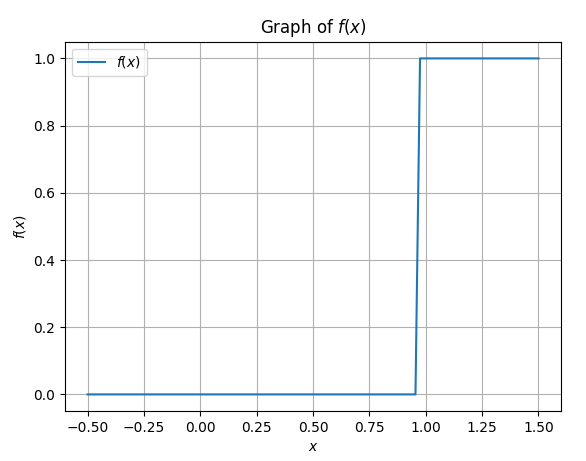
\includegraphics[width=0.6\textwidth]{Images/Cinfty function.png}
            \end{center}

            And with a little analysis, we can show that this is smooth: $\partial^m f \bigg\vert_{x=0, x= 1} = 0$ for all $m \in \N$. 


            Define $h_{\ep}(x) = f(\frac{x}{\ep})$ so $0 \leq x/\ep \leq 1$. Given $\ind_{[a, b]}$, 
            \[g_{\ep}(x) = \begin{cases}
                h(x - a - \ep) & x \leq a + \ep\\
                1 & a + \ep \leq x \leq b\\ 
                h_{\ep}(b - x) & x \geq b
            \end{cases}\]

            Clearly, $g_{\ep}(x) \to \ind_{[a,b]}$ as $\ep \to 0$.  

            And further, $0 \leq g_{\ep}(x) \leq \ind_{[a - 1, b+ 1]}$ for $\ep << 1$ so by the LDC, 
            \[\int g_{\ep}(x) \; d\mu \to \int \ind_{[a, b]} \; d\mu\] 
            or 
            \[\int \abs{g_{\ep} - \ind_{[a, b]}} \; d\mu \to \ep \]
        \end{tbox}

        \tbf{Remark:} we could also define a (more standard) \emph{Symmetric Mollifier function}
        \[\rho(x) = \begin{cases}
            \exp(- \frac{1}{1 - \abs{x}^2}) & \abs{x} < 1\\ 
            0 & \abs{x} > 1
        \end{cases}\]
        so 
        \[j = \frac{\rho}{ \int \rho \; d\mu} \int j \; d\mu = 1\]

        \begin{center}
            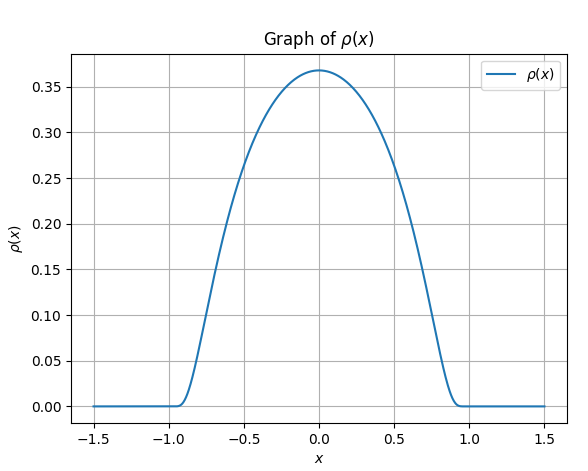
\includegraphics[width=0.6\textwidth]{Images/symmetric mollifier.png}
        \end{center}

\section*{Oct 24}
    \begin{tbox}{\textbf{Theorem (Integrals with Parameter):} Let $f(x, t): X \times [a, b) \to \C$ where $f(;, t): X \to \C$ is integrable for $t \in [a, b]$. Define 
        \[F(t) = \int f(x, t) \; d\mu\]
        \begin{enumerate}[(a)]
            \item Suppose $\exists g \in \L^1$ such that $\abs{f(x, t)} \leq g(x)$ (independent of $t$) a.e. $t$.  If $\lim_{t \to t_0} f(x, t) = f(x, t_0)$, for a.e. $t$, then 
            \[\lim_{t \to t_0} F(t) = F(t_0)\]
            In particular, if $f(x, t)$ is continuous in $t$, then $F(t)$ is continuous.
            \item Assume $\frac{\partial f}{\partial t}$ exists and $\exists g \in L^1_{\mu}$ such that 
            \[\abs{\frac{\partial f}{\partial t}(x, t)} \leq g(x)\]
            then 
            \[F'(t) = \int \frac{\partial f}{\partial t}(x, t) \; d\mu\] 
        \end{enumerate} }
        \emph{Proof:} 

        (a) Choose any $t_n \to t_0$. Define $f_n(x) = f(x, t_n)$. By assumption $\abs{f_n(x)} = \abs{f(x, t_n)} \leq g \in \L^1$. By LDC, 
        \[\lim_{n \to \infty} \int f_n(x) \; d\mu = \int \lim_{n \to \infty} f_n(x) \; d\mu = \int f(x, t_0) \; d\mu\] 

        But $t_n$ is arbitrary so
        \[\lim_{t \to t_0} \int f(x, t) \; d\mu = \int f(x, t_0) \; d\mu\]
        
        \div 

        (b) Choose 
        \[h_n(x) = \frac{f(x, t_n) - f(x, t_0)}{t_n - t_0} \]
        so for $\xi$ between $t_n$ and $t_0$,
        \[\abs{h_n(x)} = \abs{\frac{\partial f}{\partial t}(x, \xi_n)} \leq g \in L^1\]

        Once again by LDC, 
        \[\lim_{n \to \infty} \int h_n(x) \; d\mu = \int \lim h_n(x) \; d\mu = \int \partial_t f(x, t_0) \; d\mu\]
    \end{tbox}

    \subsection*{Riemann Integrals}
        \tbf{Recall:} For $f: [a, b] \to \R$, we define the Riemann integral $(R)\int_a^b f \; dx$ by 
        \begin{align*}
            S_p(f) &= \sum_{j=1}^{n} M_j (t_j - t_{j - 1})\\ 
            s_p(f) &= \sum_{j=1}^{n} m_j (t_j - t_{j - 1})\\ 
            M_j &= \sup_{[t_{j-1}, t_j]} f(x) &\qquad m_j = \inf_{[t_{j-1}, t_j]} f(x)\\ 
            \bar I_a^b &= \inf_P S_p f, \quad \underline{I}_a^b = \sup_P s_p f
        \end{align*}
        where 
        \[(R) \int_a^b f \; dx = \bar I_a^b = \underline{I}_a^b\]

        \begin{tbox}{\textbf{Theorem:} Let $f$ be a bounded real function and $\mu$ the Lebesgue measure on $\R$. 
            \begin{enumerate}[(a)]
                \item If $f$ is Riemann integrable, then $f$ is Lebesgue integrable and $(R) \int_a^b f(x) \; dx = \int_a^b f \; d\mu$
                \item $f$ is Riemann integrable $\iff \{x: f(x) \text{ not continuous on } [a, b]\}$ has Lebesgue measure zero  
            \end{enumerate} }
            \emph{Proof:} 

            (a) Notice that $\ind_{[t_j, t_{j+1}]}$ is building block of Riemann integration and $\ind_{E_j = \{j < f \leq j+1\}}$ (in general \emph{very} complicated) is the building block of Lebesgue integration.

            Assume $f$ is R-integrable. Then, $\exists P_k, P_m$ such that
            \begin{align*}
                G_{P_k} &= \sum_{j=1}^{n} M_j \ind_{(t_{j-1}, t_j]} \implies \int G_{P_k} = \sum_{j=1}^{n} M_j(t_j - t_{j-1}) = S_{P_k}(f) \\ 
                g_{P_m} &= \sum_{j=1}^{m} m_j \ind_{(t_{j-1}, t_j]} \implies \int g_{P, m} \sum_{j=1}^{m} m_j(t_j - t_{j-1}) = s_{P_m}(f)
            \end{align*}
            so 
            \begin{align*}
                \lim_{n \to \infty } \int G_{P_n} &= (R)\int_a^b f\\ 
                \lim_{m \to \infty} s_{P_m}(f) &= 0
            \end{align*}

            Now if we take a refinement $P_n \sub P_{n+1}$, $G_{P_k} \downarrow G$ and $G_{P_m} \uparrow g$ (by def as $\sup$ and $\inf$) so 
            \[(R)\int G_{P_n} \; dx \geq \int f\; d\mu \geq (R)\int g_{P_n}\;dx\]

            Taking limits, 
            \[\lim \int G_{P_n}\; dx = (R)\int_a^b f\; dx\] 
            but $\int G_{P_n}\; dx = \int G_{P_n} \; d\mu$ so using the measure theory view and the LDC, 
            \[\lim \int G_{P_n} \; d\mu = \int G \; d\mu\]

            Therefore, 
           \[(R)\int_a^b f \geq \int_a^b G \; d\mu \geq \int f \; d\mu \geq \int g \; d\mu = (R)\int d \; dx\]  
           
            So at last, $\int G \; d\mu = \int g \; d\mu \implies \int (G - g) \; d\mu \implies G = g$ a.e. 

            \div 

            \begin{exercise}
                \textbf{Homework:} Prove part (b) 
            \end{exercise}
        \end{tbox}

    \subsection*{Modes of Convergence}
        \begin{tbox}{\textbf{Egorov Theorem:} Suppose $\mu(X) < \infty$ and $f_n \to f$ a.e. Then $\forall \ep > 0$, $\exists E \sub X$ such that $\mu(E) < \ep$ with $f_n - f \to 0$ uniformly on $E^c$}
            \emph{Proof:} 

            Suppose $f_n \to f$ everywhere. 

            Recall the set of no convergence: 
            \[\phi = \{x: \exists \delta_x > 0 \st \forall N, \exists n \geq N \; \abs{f_n(x) - f(x)} \geq \delta_x\}\]

            We want to construct a uniform set to approximate $\phi$. 

            For $k \in \N$, define 
            \[E_n(k) = \bigcup_{m=n}^\infty \{x: \abs{f_m(x) - f(x)} \geq \frac{1}{k}\}\]
            so 
            \[E_n^c(k) = \bigcap_{m=n}^{\infty} \{x: \abs{f_m(x) - f(x)} \leq \frac{1}{k}\}\]

            Clearly, for fixed $k$, $E_n(k) \downarrow$ in $n$. We claim 
            \[\bigcap_{n=1}^\infty E_n(k) = \emptyset\]
            (because $\forall x \in \bigcap_{n=1}^\infty E_n(k), \; \forall n, \exists m \geq n \st \abs{f_m(x) - f(x)} \geq \frac{1}{k}$)

            Since $\mu(X) < \infty$, 
            \[\lim_{n \to \infty} \mu(E_n(k)) = \mu(\phi)\] 
            and by assumption, $\mu(E_n(k)) = 0$. 

            Now $\forall \ep > 0$, $\exists n_k < n_{k+1} \st \mu(E_{n_k}(k)) < \frac{\ep}{2^k}$. 

            Therefore, 
            \[\mu\left(\bigcup_{k=1}^\infty E_{n_k}(k)\right) < \sum_{k=1}^{\infty} \mu(E_{n_k}) \leq \ep \]

            We let $E = \bigcup_{k=1}^\infty E_{n_k}(k)$ and claim $f_n \to f$ uniformly in $E^c$. 

            We know $x \in E^c \iff x \in \bigcap_{k=1}^\infty E_{n_k}^c$ so by definition, $\forall k, \exists n_k \st \forall m \geq n_k,\; \abs{f_{m}(x) - f(x)} \leq \frac{1}{k}$. 

            \div 

            \begin{exercise}
                \textbf{Exercise:} Generalize this proof to the case $f_n \to f$ a.e. 
            \end{exercise}
        \end{tbox}

\section*{Oct 29}
    \subsection*{Modes of Convergence (Contd.)}
        \tbf{Convergence in Measure:} We say $f_n \to f$ \emph{in measure} ($f_n \overset{\mu}{\longrightarrow} f$) if $\forall \ep > 0$,
        \[\lim_{n \to \infty} \mu\{x: \abs{f_n(x) - f(x)} \geq \ep\} = 0\]

        \tbf{Convergence in $\L^1$:} We say $f_n \to f$ in $\L^1$ if $\int \abs{f_n - f} \; d\mu \to 0$.

        \begin{tbox}{\textbf{Lemma:} Assume $f_n \to f$ in $\L^1$. Then $f_n \overset{\mu}{\longrightarrow} f$}
            \emph{Proof:} 
            \[\lim \int \abs{f_n - f} \; d\mu = 0\]
            and 
            \begin{align*}
                \lim \int \abs{f_n - f} \; d\mu &\geq \int \abs{f_n - f} \ind_{\{x: \abs{f_n - f} \geq \ep\}} \; d\mu && (\text{monotonicity})\\
                    &= \int_{\{x: \abs{f_n - f} \geq \ep\}} \abs{f_n - f} \; d\mu\\
                    &\geq \int_{\{x: \abs{f_n - f} \geq \ep\}} \ep \; d\mu && (\text{monotonicity})\\ 
                    &= \ep \mu\{x: \abs{f_n - f} \geq \ep\}
            \end{align*}
            for all $\ep >0$. 

            Letting $n \to \infty$,
            \[0 = \lim \frac{1}{\ep} \int \abs{f_n - f} \; d\mu \geq \lim \mu\{x: \abs{f_n - f} \geq \ep\} \]
                        
        \end{tbox}

        \tbf{Remark:} in the proof, we have the inequality 
        \[\int \abs{f_n - f} \; d\mu \geq \ep \mu(\{x: \abs{f_n(x) - f(x)} \geq \ep\})\]
        this is the \tbf{Chebyshev Inequality}.

        \tbf{Cauchy in measure:} We say $f_n$ is \emph{Cauchy w.r.t measure} if $\forall \ep, \delta > 0$, $\exists N \st \forall n, m \geq N$, 
        \[\mu\{x: \abs{f_n(x) - f_m(x)} \geq \ep\} < \delta\]

        \begin{tbox}{\textbf{Theorem:} Assume $f_n$ is Cauchy w.r.t convergence in measure. Then $\exists f$ measurable and $f_{n_j}$ a subsequence such that $f_{n_j} \to f$ a.e. and $f_n \overset{\mu}{\longrightarrow} f$}
            \emph{Proof:} Since $f_n$ is Cauchy, $\forall j$, we may choose $f_{n_j}$ s.t. 
            \[E_j = \{x: \abs{f_{n_j}(x) - f_{n_{j+1}}(x)} \geq 2^{-j}\} \implies \mu(E_j) < 2^{-j}\]

            STEP 1. $\mu(\limsup E_j) = 0$. 

            Note $\sum_{j=1}^\infty \mu(E_j) \leq \sum_{j=1}^\infty 2^{-j} < \infty$. But by a HW, we know precisely that $\mu(\limsup E_j) = 0$.

            STEP 2. If $\forall x \notin \limsup E_j$, $f_{n_j}(x)$ is Cauchy.

            Notice that $\forall x \notin \limsup E_j = \bigcap_{j=1}^\infty \bigcup_{m=j}^\infty E_m$, $x \in \bigcup_{n=1}^\infty \bigcap_{j=n}^\infty E_j^c$. But this implies $\exists N \st \forall n \geq N$,
            \[x \in \bigcap_{j = n}^\infty E_j^c = \bigcap_{j = n}^\infty \{x: \abs{f_{n_j}(x) - f_{n_{j+1}}(x)} < 2^{-j}\}\]

            WTS $\exists j_0$ such that $j, l \geq j_0$ such that $\abs{f_{n_j}(x) - f_{n_l}(x)} < \ep$.

            WLOG, assume $n_l \geq n_j$. Now,
            \begin{align*}
                \abs{f_{n_j}(x) - f_{n_l}(x)} &\leq \sum_{j \geq l} \abs{f_{n_j}(x) - f_{n_{j+1}}(x)} + \abs{f_{n_{j+1}}(x) - f_{n_{j+2}}(x)} + \cdots + \abs{f_{n_{l-1}}(x) - f_{n_l}(x)}\\ 
                & \leq 2^{-j} + 2^{-j-1} + \cdots + 2^{-j-l}\\ 
                &\leq 2^{-j + 1}\
            \end{align*}
            and hence it is Cauchy. 

            STEP 3. $f_n \overset{\mu}{\longrightarrow} f$.

            Consider $\{x: \abs{f_n(x) - f(x)} \geq \ep\}$. We claim 
            \[\{x: \abs{f_n(x) - f(x)} \geq \ep\} \sub \{x: \abs{f_n(x) - f_{n_j}(x)} \geq \frac{\ep}{2}\} \bigcup \{x: \abs{f_{n_j}(x) - f(x)} \geq \frac{\ep}{2}\}\]
            
            Notice 
            \[\ep \leq \abs{f_n -f} \leq \abs{f_n - f_{n_j}} + \abs{f_{n_j} - f} \leq \frac{\ep}{2} + \frac{\ep}{2}\]

            So 
            \[\mu\{x: \abs{f_n(x) - f(x)} \geq \ep\} \leq \mu\{x: \abs{f_{n}(x) - f_{n_j}(x)} \geq \frac{\ep}{2}\} + \{x: \abs{f_{n_j}(x) - f(x)} \geq \frac{\ep}{2}\}\]

            But by assumption (Cauchy), $\mu\{x: \abs{f_n(x) - f(x)} \geq \frac{\ep}{2}\} \to 0$. 

            Further, 
            \[\{x: \abs{f_{n_j}(x) - f(x)} \geq \frac{\ep}{2}\} = (\limsup E_j) \cup (\limsup E_j)^c\]
            and for $j$ sufficiently large, 
            \[\{\abs{f_{n_j} - f_{n_{j+1}}} \geq 2^{-j}\} \leq 2^{-j + 1}\]
            so we are done. 
        \end{tbox}

        \tbf{Corollary 1:} If $f_n \overset{\mu}{\longrightarrow} f$, then $\exists n_j$ such that $f_{n_j} \to f$ a.e.

        \tbf{Corollary 2:} If $f_n \to f \in \L^1$, $\exists n_j$ such that $f_{n_j} \to f$ a.e.

        \tbf{Examples:} 
        \begin{itemize}
            \item For $f_n = \frac{1}{n} \ind_{[0, n]}$, $\int f_n \; d\mu = 1$ and $f_n \to 0$ uniformly but $f_n \not\to 0 \in \L^1$ 
            
            \item For $f_n = \ind_{[n, n+1]}$, $\int f_n \; d\mu = 1$ and $f_n \to 0$ a.e. but 
            \[\int \abs{f_n - f} \; d\mu = \int \abs{f_n} \; d\mu = 1 \neq 0\] 
            so $f_n \not\to 0$ in $\L^1$. Do we at least have convergence in measure? No: 
            \[\mu\{x: \abs{f_n(x) - 0} > \frac{1}{2}\} = \mu(n, n+1) = 1\]

            \item $f_n = n \ind_{[0, \frac{1}{n}]}$. 
        
            As before, $\int f_n \; d\mu = 1$ and $\forall x_0 \neq 0$, $\exists n_{x_0} \st \forall n \geq n_{x_0}$, $f_n(x_0) = 0$ so $f_n \to 0$ a.e. By the same argument, we can say $f_n \not\to f$ in $\L^1$.  

            However, $\mu\{x: \abs{f_n(x) - 0} > \ep\} = \mu[0, \frac{1}{n}] = \frac{1}{n} \to 0$ so $f_n \overset{\mu}{\longrightarrow} 0$.
        \end{itemize}

\section*{Oct 31}
    \tbf{Recall:} last time, we showed that if $f_n \overset{\mu}{\longrightarrow} f$, then $\exists n_j$ such that $f_{n_j} \to f$ a.e.

    \begin{proof}
        \emph{Proof Sketch:} Suffices to show 
        \[\lim_{j \to \infty} \mu\{\abs{f_{n_j} -f } \geq \frac{\ep}{2}\} = 0\]

        By construction, $\exists j_0$ such that $\forall j \geq j_0$,
        \[\bigcap_{j\geq j_0}^{\infty} E_{n_j}^c \iff \abs{f_{n_j} - f} \leq 2^{-j+1}\] 
        (strict inequality is not preserved in the limits)
        
        But also, 
        \[\bigcup_{j\geq j_0}^\infty E_{n_j}^c \iff \abs{f_{n_j} - f} \geq 2^{-j + 1}\]
        so 
        \[\mu\{\abs{f_{n_j} - f} \geq \frac{\ep}{2}\} \leq \mu\{\abs{f_{n_j}  -f} \geq 2^{j+1}\} \leq \sum_j^{\infty} \mu(E_{n_j}) \leq 2^{-j+1}\]
    \end{proof}

    \tbf{Remark:} we have actually shown a stronger result: $f_{n_j} - f \to 0$ as $\mu(E_{n_j}) \to 0$. Technically, it suffices to show that they both go to $0$ -- not that it happens at the same time.

    \subsection*{Example (Moving intervals)} 
        Let $f_1 = \ind_{[0, 1]}$, $f_2 = \ind_{[0, 1/2]}$, $f_3 = \ind_{[1/2, 1]}$, $f_4 = \ind_{[0, 1/4]}$, $f_5 = \ind_{[1/4, 1/2]}$, $f_6 = \ind_{[1/2, 3/4]}$, $f_7 = \ind_{[3/4, 1]}$ etc.

        Assume $n = 2^k + j$ with $j < 2^k$, then 
        \[f_n = \ind_{[\frac{j}{2^k}, \frac{j+1}{2^k}]}\]

        Note that the support of the intervals is shrinking to $0$!

        We claim:
        \begin{enumerate}
            \item $f_n \overset{\mu}{\longrightarrow} 0$ 
            
            \begin{proof}
                \emph{Proof:} $\mu\{\abs{f_n} > \ep\} \leq \mu\{x: f_n(x) \neq 0\} \to 0$
            \end{proof}

            \item $f_n \not\to 0$ a.e. 
            
            \begin{proof}
                \emph{Proof:} $\forall x_0$, $\exists k$ such that $x_0 \in [\frac{j}{2^k}, \frac{j+1}{2^k}]$ for some $j$ (nested interval). But then $f_n(x_0) = 1$ on a set with measure $2^{-k} > 0$.
            \end{proof}
        \end{enumerate}

    \subsection*{Product Measures}
        Let $(X, \M, \mu)$ and $(Y, \Nc, \nu)$ be two measure spaces. We want to construct a canonical product measure $\mu \times \nu$. 
        
        Intuitively, it would be very nice if for $A \in \M$, $B \in \Nc$, $\mu(A \times B) = \mu(A) \nu(B)$

        \tbf{Recall:} We have earlier defined $\M \otimes \Nc$ to be the $\sigma$-algebra generated by the rectangles $A \times B$ with $A \in \M$, $B \in \N$.

        \tbf{Facts:} 
        \begin{enumerate}
            \item $A \times B \cap (E \times F) = (A \cap E) \times (B \cap F)$
            \item $(A \times B)^c = (X \times B^c) \cup A^c \times B = (A \times B^c) \cup (A^c \times B^c) \cup (A^c \times B)$
        \end{enumerate}

        Let $\A$ be the finite union of rectangles $A \times B$. By the fact, $\A$ is closed under (finite) complements, hence is an algebra. 

        \begin{tbox}{\textbf{Lemma:} Assume for $A \in \M$, $B \in \Nc$ with $\mu(A), \mu(B) < \infty$, 
            \[A \times B = \bigcup_{i=1}^\infty A_i \times B_i\]
            with $(A_i \times B_i) \cap (A_j \times B_j) = \emptyset$ for $i \neq j$. Then
            \[\mu(A)\nu(B) = \sum_{i=1}^{\infty} \mu(A_i) \nu(B_i)\]}
            \emph{Proof:} 

            By a property of the characteristic function, 
            \[\ind_{A \times B}(x, y) = \ind_A(x) \cdot \ind_B(y)\]

            We claim 
            \[\ind_A(x) \cdot \ind_B(y) = \sum_{i=1}^{\infty} \ind_{A_i \times B_i}(x, y)\]
            (\emph{Proof:} Self evident by pairwise disjoint) 

            But then 
            \[\sum_{i=1}^{\infty} \ind_{A_i \times B_i}(x, y) = \sum_{i=1}^\infty \ind_{A_i}(x) \cdot \ind_{B_i}(y)\]

            Fix $x$ and consider: as functions of $y$, the characteristic function is measurable. Hence, by the series version of MCT, 
            \[\ind_A(x) \nu(B) = \sum_{i=1}^\infty \ind_{A_i}(x) \cdot \nu(B_i)\]

            But now this is just a function of $x$, so by the same argument,
            \[\mu(A) \nu(B) = \sum_i \mu(A_i) \nu(B_i)\]

            But this order was arbitrary! Instead fix $y$. By MCT with respect to $x$, 
            \[\mu(A) \ind_B(y) = \sum_i \mu(A_i) \cdot \ind_{B_i}(y)\]
            and then integrating over $y$, 
            \[\mu(A) \nu(y) = \sum_i \mu(A_i) \nu(B_i)\]
            which is exactly the same! 

            This is the essence of Fubini's Theorem.
        \end{tbox}

        \tbf{Remark:} the condition for this lemma is highly nontrivial. In general, it is extremely difficult to cover an arbitrary space in disjoint rectangles (see an earlier HW)

        Now it remains to actually construct the product measure such that 
        \[\mu \times \nu(A \times B) = \mu(A) \nu(B)\]

        \tbf{Premeasure:} we call $\mu_0$ a \emph{Premeasure} if for $A = \bigcup_{i=1}^\infty A_i$ with $\mu_0(A_i)$ well defined, 
        \[\mu_0(A) = \sum_{i=1}^\infty \mu_0(A_i)\]

        Recall the outer measure 
        \[\mu^*(E) = \inf \sum_i \rho(A_i)\]
        for $E \sub \bigcup_i A_i$ which immediately gives us a measure by Carathéodory. 

        Let's try to replicate this. Let $\mu(A \times B) = \mu(A) \nu(B)$ be set functions on $\A$, the set of finite disjoint unions of rectangles $A \times B$. 
        
        Define
        \[\mu^*(E) = \inf \sum_i \mu(A_i) \nu(B_i)\]
        for $E \sub \bigcup_i A_i \times B_i$. By results earlier in the class, this is an outer measure which gives us a measure $\mu \times \nu$. 

        \begin{tbox}{\textbf{Lemma:}
            \begin{enumerate}
                \item $\mu \times \nu(A \times B) = \mu(A) \nu(B)$
                \item $\A$ is $\mu\times \nu$-measurable
            \end{enumerate}}
            \emph{Proof:} 

            1. Let $A \times B \sub \A$ and suppose $A \times B \sub \bigcup_{i=1}^\infty A_i \times B_i$. 

            Clearly, 
            \[A \times B = (A \times B) \cap \left(\bigcup_{i=1}^\infty A_i \times B_i\right) = \bigcup_{j=1}^\infty (A\times B \cap A_i \times B_i)\]
            Let $B_n = E \cap \left(\bigcup_{i \in I} A_i \right)$

            By the earlier lemma, 
            \[\sum_{i=1}^\infty \mu(A \cap A_i) \nu(B \cap B_i) = \mu(A) \nu(B)\] 

            Therefore, 
            \[(\mu \times \nu)(A\times B) \geq \mu(A) \nu(B)\]

            But also, for any $A\times B$, take its trivial covering so 
            \[(\mu \times \nu) (A \times B) \leq \mu(A) \nu(B)\]
        \end{tbox}

\section*{Nov 7}
    \tbf{Recall:} For measure spaces $(X, \M, \mu)$ and $(Y, \Nc, \nu)$, we would like to construct a product measure $\mu \times \nu$ on $X \times Y$ such that
    \[\mu\times\nu(A \times B) = \mu(A)\mu(B)\]

    Last time, we showed that this is true on $\A$, a finite union of disjoint rectangles $A_i \times B_i$: 
    \[A \times B = \bigcup_{i=1}^\infty A_i \times B_i \implies \mu\times\nu(A \times B) = \sum_{i=1}^\infty \mu(A \cap A_i) \nu(B \cap B_i)\]

    By our construction, the $\mu_0$ that satisfies this property is a \emph{premeasure} (i.e. it is countably additive but not necessarily defined on a $\sigma$-algebra). It would be very nice if we could extend this to all of $\M \otimes \Nc$ (just as we did for Outer Measures with Carathéodory).

    And in fact, it is not too difficult. First recall that, in general,
    \[\mu^*(E) = \inf_{\bigcup_i A \supseteq E} \sum_{j=1}^\infty \mu_0(A_j)\]
    is an outer measure. We then invoke Carathéodory's Theorem to get a measure $\mu$ on $\M \otimes \Nc$ and we are done.

    All that remains are a few specifics:

    \begin{tbox}{\textbf{Proposition:} If $\mu_0$ is a premeasure on $\A$, then for $\mu^*$ defined by
    \[\mu^*(E) = \inf_{\bigcup_i A \supseteq E} \sum_{j=1}^\infty \mu_0(A_j)\]
    \begin{enumerate}
        \item $\mu^*\big|_{\A} = \mu_0$
        \item $\A$ is $\mu^*$-measurable
    \end{enumerate}}
    
        \emph{Proof:} 

        1. Take a set $E \sub A$. By choosing $E$ as its own cover, $\mu^*(E) \leq \mu_0(E)$ by the inf. 

        Conversely, take any cover $\bigcup_{j=1}^\infty A_j \supseteq E$. WLOG, $A_j$ are disjoint (or else we can repeat the argument with $B_j = \bigcup_{j=1}^\infty A_j \setminus A$). 

        \begin{exercise}
            \textbf{Exercise:} Verify the case where $A_j$ are not disjoint.
        \end{exercise}

        Then,
        \[\bigcup_{j=1}^\infty A_j \cap E = E \sub \A \implies \sum_{j=1}^\infty \mu(A_j \cap E) = \mu_0(E)\]
        since $\mu_0$ is a premeasure.

        But we know also 
        \[\sum_{j=1}^\infty \mu_0(A_j) \geq \sum_{j=1}^\infty \mu_0(A_j \cap E)\]
        so by def of inf, 
        \[\mu_0(E) \geq \inf \sum \mu_0(A_j) = \mu^*(E)\]

        \div 

        2. Choose a test set $E \sub P(X \times Y)$. Then, by definition, $\exists B_j^{\infty} \in \A$ such that for $E \sub \bigcup_j B_j$,
        \[\mu^*(E) + \ep > \sum_j \mu_0(B_j) = \sum_j \mu_0(B_j \cap A) + \mu_0(B_j \cap A^c)\]
        (disjoint since $B_j \in \A$)

        But now the first term gives us a cover for $E \cap A$ and the second term gives us a cover for $E \cap A^c$.

        Certainly,
        \[\sum_j \mu_0(B_j \cap A) + \mu_0(B_j \cap A^c) \geq \mu^*(E \cap A) + \mu^*(E \cap A^c)\]
        
    \end{tbox}

    We now want two more powerful properties: uniqueness and faithfulness. 

    \begin{tbox}{\textbf{Theorem (Uniqueness of Extension):} Let $\A \sub P(X)$ be an algebra, $\mu_0$ a premeasure. Let $\M$ be the $\sigma$-algebra generated by $\A$ and $\mu$ the extension of $\mu_0$ to $\M$. If $\nu$ is another measure on $\M$ that agrees with $\mu_0$ on $\A$, then $\nu(E) \leq \mu(E)$ for all $E \in \M$ with $\mu(E) < \infty$}
        \emph{Proof:} 

        STEP 1. Let $E \sub \M$ with $E \sub \bigcup_{j=1}^\infty A_j$ for $A_j \in \A$. Then,
        \[\nu(E) \leq \sum_{j=1}^\infty \nu(A_j) = \sum_{j=1}^\infty \mu_0(A_j)\]
        which implies $\nu(E)$ is a lower bound (by $\mu^*$ definition). 

        Hence, $\nu(E) \leq \mu(E)$. 

        STEP 2. $\mu(A) = \nu(A)$ for $A = \bigcup_{j=1}^\infty A_j$.

        We note
        \[\bigcup_{j=1}^\infty A_j \nearrow A\]

        By taking the limit 
        \[\nu(A) = \lim_{n \to \infty} \nu(\bigcup_{j=1}^n A_j) = \lim_{n \to \infty} \mu(\bigcup_{j=1}^n A_j)\]

        STEP 3. Take $A = \bigcup_{i=1}^\infty A_j$ such that $E \sub \bigcup_j A_j$ so 
        \[\mu(A) \leq \mu(E) + \ep \implies \mu(A \setminus E) < \ep\]

        We claim $\mu(E) \leq \nu(E)$:
        \begin{align*}
            \mu(E) &\leq \mu(A) = \nu(A)\\
                &= \nu(E) + \nu(A \setminus E)\\ 
                &\leq \nu(E) + \mu(A \setminus E)\\ 
                &< \nu(E) + \ep\\ 
                &\overset{\ep \to 0}{\longrightarrow} \nu(E)
        \end{align*}

        STEP 4.

        \begin{exercise}
            \textbf{Exercise:} Prove that $\mu$ is $\sigma$-finite.
        \end{exercise}
    \end{tbox}

    \begin{tbox}{\textbf{Corollary:} Lebesgue Product Measure }
        \emph{Proof:} HW (Construct a product measure via cubes). 

        By uniqueness, the measure from HW and the measure here are the same. 
    \end{tbox}

\subsection*{Fubini's Theorem}
    Consider $E \sub \M \otimes \Nc$. For all $x$, take sections of $E$:
    \[E_x: \{y \in Y: (x, y) \in E\}\]
    and similarly for $y$:
    \[E_y: \{x \in X: (x, y) \in \E\}\]

    \begin{center}
    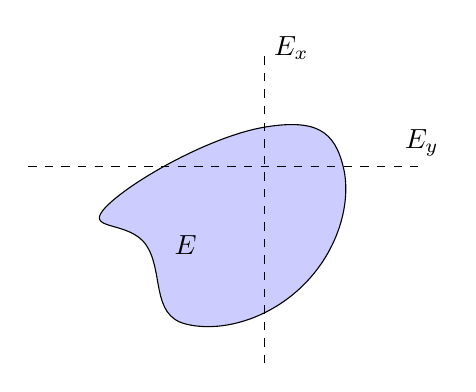
\begin{tikzpicture}
        % Draw the blob-shaped set E
        \draw[fill=blue!20] plot [smooth cycle, tension=0.8] coordinates {(0,0) (2,1) (3,0.5) (2.5,-1) (1,-1.5) (0.5,-0.5)};

        % Draw the vertical line E_x
        \draw[dashed] (2, -2) -- (2, 2);
        \node[right] at (2, 2) {$E_x$};

        % Draw the horizontal line E_y
        \draw[dashed] (-1, 0.5) -- (4, 0.5);
        \node[above] at (4, 0.5) {$E_y$};

        % Label the set E
        \node at (1, -0.5) {$E$};

    \end{tikzpicture}
    \end{center}

    \begin{tbox}{\textbf{Lemma:}
        \begin{enumerate}
            \item $E \in \M \otimes \Nc \implies E_x \in \Nc$ and $E_y \in \M$
            \item If $f(x, y)$ is a measurable function on $\M \otimes \Nc$, then $f_x(x,y)$ is measurable on $y$ and $f^y(x,y)$ is measurable on $x$.
        \end{enumerate} }
        \emph{Proof:} 

        1. Define $R = \{\forall x,\; E_x \in \Nc, \land \forall y, \; E_y \in \M\}$. It suffices to show that $R \supseteq \M \otimes \Nc$.

        By the previous lemma, $\A \sub R$. 

        \begin{exercise}
            \textbf{Exercise:} Check that $R$ is a $\sigma$-algebra. (Hint: $\M$ and $\Nc$ are $\sigma$-algebras)
        \end{exercise}

        But by definition, $\M \otimes \Nc$ is generated by $\A$ (hence the smallest $\sigma$-algebra containing $\A$), so $R \supseteq \M \otimes \Nc$.

        2. $(f_x)^{-1}(B) = (f^{-1}(B))_x$ and $(f^y)^{-1}(A) = (f^{-1}(A))^y$ by properties of the preimage. 

        \begin{exercise}
            \textbf{Exercise:} Check that the preimage properties hold 
        \end{exercise}

        By part 1, $f_x$, $f_y$ are measurable.
    \end{tbox}

    \begin{tbox}{\textbf{Fubini-Tonelli Theorem:} Let $(X, \M, \mu)$ and $(Y, \Nc, \nu)$ be $\sigma$-finite measure spaces. If $f \in \L^+(X \times Y)$, then $g(x) = \int f_x \;d\nu$ and $h(y) = \int f^y\; d\mu$ satisfies 
        \[\int f \; d\mu \times \nu = \int\left[\int f(x, y) \; d\nu(y)\right] \; d\mu(x) = \int\left[\int f(x, y) \; d\mu(x)\right]\; d\nu(y)\]}
        \emph{Proof of Weak Form:} By dyadic approximation, it suffices to consider $\ind_E \approx \ind_A$ 
        
        STEP 1. If $\mu \times \nu(E) = 0$, then $\nu(E^x) = 0$ for almost every $x$ WRT $\mu$. Similarly, $\mu(E^y) = 0$ for almost every $y$ WRT $\nu$.

        Since $\mu \times \nu(E) = 0$, choose $A_n \in \A$, $\mu \times \nu(A_n) \to 0$ so for $E \sub A_n$, 
        \[\ind_E \leq \ind_{A_n} \implies \ind_{E_x} \leq \ind_{A_{n_y}} \implies \ind_E(y) \leq \ind_{A_n}(y)\] 

        Therefore, 
        \[\int \nu(E_x) = \int \int \ind_{E_x} \; d\nu\; d\mu \leq \int \int \ind_{A_{n_x}} \; d\nu \; d\mu = \mu\times \nu(A_n) \overset{n\to\infty}{\longrightarrow} 0\]
        and $\int \mu(E^y)$ follows similarly.

        STEP 2. For $\ind_E$, we have $\ind_{A_n}$ such that $E \sub A_n$ and $\mu(E \setminus A_n) \to 0$. Hence, $\ind_{A_n} \to \ind_E$ in $\L^1(\mu \times \nu)$. By Chebyshev, it follows that $\ind_{A_n} \to \ind_E$ in measure. Hence, $\exists A_{n_k}$ such that $\ind_{A_{n_k}} \to \ind_E$ a.e. (WRT $\mu \times \nu$). So $\exists E^0$ with $\mu(E^0) = 0$ such that $\ind_{A_{n_k}} \to \ind_E$ on $E\setminus E^0$. 

        But then, 
        \[\int_{X \times Y \setminus E^0} \ind_{A_n} \; d\mu\times \nu = \int_{X \times Y \setminus E^0} (\ind_{A_n} \; d\mu) \; d\nu = \int_{X \times Y \setminus E^0}(\ind_{A_n} \; d\nu) \; d\mu\]
        (since $E^0$ has measure $0$)

        Taking $n \to \infty$, everything is bounded and in $\L^1$ so by LDC, 
        \[\int_{X \times Y \setminus E^0} \ind_{B}; d\mu\times \nu = \int_{X \times Y \setminus E^0} (\ind_{B} \; d\mu) \; d\nu = \int_{X \times Y \setminus E^0}(\ind_{B} \; d\nu) \; d\mu\]
        and hence 
        \[\int_{X \times Y} \ind_{B}; d\mu\times \nu = \int_{X \times Y} (\ind_{B} \; d\mu) \; d\nu = \int_{X \times Y}(\ind_{B} \; d\nu) \; d\mu\]

        STEP 3. Recall the dyadic approximation $0 \leq f \in \L^1(\mu \times \nu)$ and $f_n \nearrow f$ pointwise where $f_n$ are simple functions. 

        Clearly, step 2 should hold for $f_n$. Hence,
        \[\int \int f_n \; d\mu \; d\nu = \int \int f_n \; d\nu \; d\mu\]

        We can also take sections $f_{n_x} \nearrow f_x$ and $f_{n}^y \nearrow f^y$ so taking the limit, 
        \[\int \int f \; d\mu \; d\nu = \int \int f \; d\nu \; d\mu\]
    \end{tbox} 

    \tbf{Remark:} This works just fine for integration in general but we would still like a more general result that does not depend on losing a measure $0$ set. 

\section*{Nov 12}
    Last time, we gave a weak form of the proof of the Tonelli Theorem:
    \begin{enumerate}
        \item $(\mu \times \nu)E = 0 \implies \mu(E^y)= 0, \; \nu(E^x) = 0$ and measurable
        \item By approximation of $\inf$ and $A_n$ disjoint union,
        \[\norm{\ind_{A_n} - \ind_E}_{\L^1} \to 0 \implies \ind_{A_{n_k}} \to \ind_E \text{ a.e.}\]
        \item Choose a zero measure set $E_0$ so $(\mu \times \nu)E_0 = 0$ and $\ind_{A_{n_k}} \to \ind_E$ on $E \setminus E_0$. Hence, 
        \[\ind_{A_{n_k} \cap E_0^c} \to \ind_{E \cap E_0^c}\]
        pointwise. 

        \item Now, 
        \[\int \ind_{A_{n_k}} \; d\mu \; d\nu = \int (\int \ind_{A_{n_k}} \; d\mu) \; d\nu = \int (\int \ind_{A_{n_k}} \; d\nu) \; d\mu\]
        as $k \to \infty$,
        \[\int \ind_{E \setminus E_0} \; d\mu \; d\nu = \int (\int \ind_{E \setminus E_0} \; d\mu) \; d\nu = \int (\int \ind_{E \setminus E_0} \; d\nu) \; d\mu\]

        Using LDC, 
        \[\int \ind_E \; d\mu \; d\nu = \int \int \ind_E \; d\mu \; d\nu = \int \int \ind_E \; d\nu \; d\mu\]
    \end{enumerate}

    But this still sacrifices a set of measure $0$. We will offer a new proof that uses monotone convergence instead of convergence in norm. 

    But first, a lemma. 

    \tbf{Monotone Class over $X$:} $\Cc \sub P(x)$ is a \emph{monotone class} if
    \begin{itemize}
        \item for $E_n \in \Cc$ and $E_n \nearrow$, then $\bigcup_{n=1}^{\infty} E_n \in \Cc$
        \item OR for $E_n \in \Cc$ and $E_n \searrow$, then $\bigcap_{n=1}^{\infty} E_n \in \Cc$
    \end{itemize}

    \begin{tbox}{\textbf{Lemma:} Consider $A \sub P(X)$, an algebra. We consider the sigma algebra $\M = \M(A)$ and the monotone class $\Cc = \Cc(A)$ generated by $A$. Then $\M = \Cc$.}
        \emph{Proof:} By definition, every $\sigma$-algebra is a monotone class so the smallest monotone class cannot be larger than the smallest $\sigma$-algebra: $\Cc \sub \M$.

        Hence, it suffices to show that $\Cc$ is a $\sigma$-algebra. 

        STEP 1. Consider $\Cc(E) = \{F \sub \Cc: E \setminus F,\, F \setminus E,\, E \cap F \in \Cc\}$.

        Clearly, $\emptyset \in \Cc(E)$ and $E \in \Cc(E)$.

        Further, since we have the symmetric difference, $F \in \Cc(E) \iff E \in \Cc(F)$. 

        We also know that $\Cc(E)$ is a monotone class since if $F_n \nearrow F_{\infty}$, $E \setminus F \searrow$. Similarly, $F \setminus E \nearrow$ for $F_n \searrow F_{\infty}$.

        STEP 2. For $E \sub A$, then $F \in \Cc(E)$ for all $F \in A$ (since $A$ is an algebra). Therefore, $A \sub \Cc(E) \implies \Cc(A) \sub \Cc(E)$ 

        STEP 3. $\Cc(A)\sub \Cc(F)$ for any $F \in \Cc$. Then $\forall F \in \Cc$, $F \in \Cc(E)$ for any $E \sub A$. 

        By symmetry, $E \sub \Cc(F)$. Hence, $\Cc(A) \sub \Cc(F)$ which implies $\Cc(A)$ is an algebra. 
        
        STEP 4.

        \begin{exercise}
            \textbf{Exercise:} Show $\Cc(A)$ is a $\sigma$-algebra
        \end{exercise}
    \end{tbox}

    \tbf{Remark:} This is incredibly powerful because it means we can always approximate a $\sigma$-algebra by monotone sets. 
    
    \begin{tbox}{\textbf{Tonelli Theorem}: 
        \[\int \ind_E \; d\mu \; d\nu = \int \left(\int \ind_E \; d\mu\right) \; d\nu = \int \left(\int \ind_E \; d\mu\right) \; d\nu\]}
        \emph{Strong form of the Proof:} WLOG, assume $\mu, \mu$ are finite (or else just approximate). 
        
        Denote $\Cc = \{\text{all sets } E \text{ s.t. the theorem holds}\}$.

        Certainly, $A \sub \Cc$ (basic lemma). 

        We claim $\Cc$ is a monotone class, i.e. $E_n \nearrow E_{\infty}$ or $E_n \searrow E_{\infty}$ implies $E_{\infty} \in \Cc$. In fact, by construction, $\ind_{E_n} \nearrow \ind_{E_{\infty}}$ so taking sections, 
        \[\begin{cases}
            \ind_{E_{n_x}} \nearrow \ind_{E_{\infty_x}} \quad \text{OR} \quad \ind_{E_{n_x}} \searrow \ind_{E_{\infty_x}}\\ 
            \ind_{E_{n}^y} \nearrow \ind_{E_{\infty}^y} \quad \text{OR} \quad \ind_{E_n^y} \searrow \ind_{E_{\infty}^y}
        \end{cases}\]
        
        Now taking the limits (and using finite measure in the $\searrow$ case), 
        \[\int \ind_{E_{\infty}} \; d\mu \; d\nu = \int \left(\int \ind_{E_{\infty}} \; d\mu\right) \; d\nu = \int \left(\int \ind_{E_{\infty}} \; d\mu\right) \; d\nu\] 
        so $E_{\infty} \sub \Cc$. 

        By the monotone class lemma, $\M = \Cc$. 

    \end{tbox}

\section*{Nov 14}
\subsection*{The Lebesgue Measure on $\R^n$}
    Denote $m$ the Lebesgue measure and $\L^n$ the class of Lebesgue measurable sets.

    \begin{tbox}{\textbf{Theorem (Approximation):} If $E \in \L^n$,
        \begin{enumerate}
            \item $m(E) = \inf \{m(U): E \sub U, \; U \text{ open}\} = \sup\{m(K): K \sub E, \; K \text{ compact}\}$
            \item $E = A_1 \cup N_1 = A_2 \setminus N_2$, where $A_1$ is a $F_{\sigma}$ set (i.e. union of open sets), $A_2$ is a $G_{\delta}$ set (i.e. intersection of closed sets), and $m(N_1) = m(N_2) = 0$. (In particular, $A_1$ and $A_2$ are Borel sets).
            \item If $m(E) < \infty$, then $\forall \ep > 0$, there exists a finite collection of disjoint rectangles such that 
            \[m\left(E \triangle \bigcup_{j=1}^N R_j\right) < \ep \]
        \end{enumerate}}
        \emph{Proof Sketch:}
        
        1) $\forall \ep > 0$, take a covering by disjoint rectangles $A_j \in \A$ such that $m(E) \leq \sum m(A_j) < m(E) + \ep$. For each $j$, choose an open set $U_j$ s.t. $m(U_j) \leq m(A_j) + \ep 2^{-j}$ and $A_j \sub U_j$. Now
        \[E \sub U = \bigcup_{j=1}^\infty U_j \implies \sum_{j=1}^\infty m(U_j) <m(E) + 2\ep \implies m(E) = \inf \{m(U): E \sub U\}\]

        The proof for $\sup$ follows immediately from the 1-D proof earlier in the course. 

        2) Follows from Part 1 and the midterm

        3) We may split $A_j$ into very small sets $\delta$ so 
        \[m(E) \leq \sum_1^N m(A_j) + \sum_N^{\infty} m(\delta) < m(E) +\ep\] 

        Choosing $N$ large and using the finitude of $m(E)$,
        \[m(E) - \ep < \sum_1^N m(A_j) < m(E) + \ep\]

    \end{tbox}

    \tbf{Corollary of 3 (Lusin's Theorem):} (globally defined) smooth functions approximate each $\ind_{V_j}$:
    \[\norm{\sum_{i=1}^N \ind_{V_j} - \ind_E}_{L^1} < \ep\]

    \begin{tbox}{\textbf{Approximation for $\L^1$ functions (1D general):} If $f \in \L^1(m)$, let $\ep > 0$, then there exists a simple function $\phi = \sum_1^N a_i \ind_{R_j}$ for $R_j$ disjoint rectangles such that 
    \[\int \abs{f - \phi} < \ep\]
    In particular, we can choose a continuous function $f_c$ with compact support such that 
    \[\int \abs{f_c - \phi} < \ep\]}
        \emph{Proof Sketch:} It suffices to consider $\ind_E = \ind_{\bigcup_{j=1}^N R_j}$. 

        By approximation of sets and smoothness of product of 1D mollifiers, we can approximate $\ind_E$ by a smooth function. Further, the support of these functions are disjoint. 

    \end{tbox}

\subsection*{Dyadic Cubes}
    Let $Q_k$ the dyadic cube (an n-D closed rectangle with same sides) of length $2^{-k} \Z$. Conveniently, $Q_{k+1} \sub Q_k$. 

    Let $E \sub \R^n$. Define 
    \begin{align*}
        \underbar A(E, k) &= \bigcup Q \sub Q_k && Q_k \sub E\\ 
        \bar A(E, k) &= \bigcup Q \sub Q_k && Q_k \cap E \neq \emptyset 
    \end{align*}
    clearly, $\underbar A \sub \bar A$ so $m(\underbar A(E, k)) \leq m(\bar A(E, k))$. 

    Hence, $\underbar A(E, k) \nearrow_k$ and $\bar A(E, k) \searrow_k$.

    Define $\underbar A(E) = \lim_k \underbar A(E, k)$ and $\bar A(E) = \lim_k \bar A(E, k)$. If $\underbar A(E) = \bar A(E)$, then we say $E$ has the same \tbf{Jordan content}

    \begin{tbox}{\textbf{Lemma:} Let $U$ be open, then $U = \underbar A(U)$. Moreover, $U$ is a countable union of disjoint cubes}
        \emph{Proof:} Fix $x \in U$. Define $\delta = \inf_{y \setminus U} \abs{y - x} > 0$. We know $B_{\delta}(x) \sub U$. Therefore, there exists a cube containing $x$ that is contained in $B_{\delta}(x)$.

        For large $k$, $x \in \underbar A(U_k) \sub \underbar A(U)$.

        The other direction is trivial.

        By the nature of dyadic cubes, $\underbar A(U)$ is a countable collection $\bigcup_{k=0}^{\infty} A(U, k) = \underbar A(U)$. 

        We can rewrite 
        \[\bigcup_{k=0}^{\infty} A(U, k)  = A(U, 0) \bigcup_{k=1}^\infty \{\underbar A(U, k) \setminus \underbar A(U, k-1)\}\]
        which ensures we have a disjoint union. 
    \end{tbox}

\subsection*{Change of Variables}
    \tbf{Remark:} one reasonably intuitive way is to:
    \begin{itemize}
        \item Show change of variables for Riemann integration 
        \item Show that for smooth functions, Lebesgue and Riemann integration is the same.
        \item Show that for $\L^1$ functions, we can approximate by smooth functions.
    \end{itemize} 
    where the main difficulty is generalizing the Riemann-Lebesgue correspondence past 1D. 

    However, we will take a more measure theoretic approach. 

    \begin{tbox}{\textbf{Theorem (Translation Invariance):} Let $\tau_a(x) = x + a$ for $a \in \R^n$. Then,
        \begin{enumerate}
            \item $m(\tau_a(E)) = m(E)$
            \item If $f: \R^n \to \C$ is either $\geq 0$ or in $\L^1$, 
            \[\int f(x + a)\; d\mu= \int f\; d\mu \]
        \end{enumerate}}
        \emph{Proof sketch:} 
        
        1) For rectangles, $m(A) = m(\tau_a(A))$. We claim this holds for general sets because $\tau_a$ is a bijection between $E(x + a)$ and $E$ and also $A(x + a)$ and $A(x)$.
        
        2) This gives us the result for the characteristic function which immediately gives us simple functions (and thus $\L^1$ functions by approximation).

    \end{tbox}

\section*{Nov 19}
    \tbf{Recall:} Last time we showed that if $U$ is open, $U = \underbar A(U)$, a collection of dyadic cubes.

    \begin{tbox}{\textbf{Corollary:} Let $U$ be open, then the \tbf{inner content} is $m(U) = m(\underbar A(U))$. Let $F \sub \R^n$ be a compact set. Then the \tbf{outer content} is $m(F) = m(\bar A(F))$.} 
        \emph{Proof Sketch:} Define $Q_0 = \{x: \max\abs{x_j} \leq 2^M, \; M\}$ for $M$ sufficiently large. We have $F \in Q_0$. 

        Consider $Q_k$, the $2^{-k}$ dyadic cubes. For any $Q \sub Q_k \land Q \sub Q_0$, then either $Q \cap F = \emptyset$ or $Q \sub Q_0\setminus F$ so that 
        \[m(\bar A(F, k)) + m(\underbar A(Q_0 \setminus F, k)) = m(Q_k) = m(Q_0)\]

        But $Q_0 \setminus F$ is open so taking $k \to \infty$, the result follows from the lemma.
    \end{tbox}

    \begin{tbox}{\textbf{Theorem:} Let $\Omega \sub \R^n$ be open. Let $G: \Omega \inj \R^n$ be $C^1$ differentiable (i.e. the jacobian $D_x G \in C^1$) and invertible. 
        \begin{enumerate}
            \item If $E \sub \Omega$, $E \in \L^n$, $G(E) \in \L^n$, then 
            \[\int_{G(E)} \ind_{G(E)} = m(G(E)) = \int_E \abs{\det D_x G} \ind_E \; dx\]
            \item If $f \in \L^1(G(\Omega))$, $f \circ G \in L^1(\Omega)$, and $f \geq 0$, 
            \[\int_{G(\Omega)} f(y)\; dy = \int_{\Omega} f \circ G(x) \abs{\det D_xG} \; dx\]
        \end{enumerate}}
        \emph{Proof:} 

        1. WLOG assume $m(E) < \infty$ (else invoke $\sigma$-finitude). 

        STEP 1. (Translation Invariance). 
        
        Define $\tau_a(x) = x + a$ for $a \in \R^n$. WTS, 
        \[m(E) = m(\tau_a(E))= m(\{x + a: x \in E\})\]

        \begin{proof}
            \emph{Proof:} This is exactly the same as the 1D proof:
            \begin{itemize}
                \item True for rectangles 
                \item $\inf$ structure of $m$ implies a bijection between $E$ and $\tau_a(E)$
            \end{itemize}
        \end{proof}

        STEP 2. Let $T_1, T_2, T_3$ be elementary linear maps:
        \begin{align*}
            T_1: (x_1, \dots, x_j, \dots, x_n) &\mapsto (x_1, \dots, cx_j, \dots, x_n)\\
            T_2: (x_1, \dots, x_j, \dots, x_n) &\mapsto (x_1, \dots, x_j + cx_k, \dots, x_n), \quad j \neq k \\
            T_3: (x_1, \dots, x_i, x_j, \dots, x_n) &\mapsto (x_1, \dots, x_j, x_i, \dots, x_n)
        \end{align*}

        WTS, $m(T(E)) = \det\abs{T} m(E)$ where $T \in \{T_1, T_2, T_3\}$. 

        \begin{proof}
            \emph{Proof:} Consider 
            \begin{align*}
                m(T_1(E)) &= \int \ind_{T_1(E)}\\ 
                    &= \int \ind_{(x_j, \dots, cx_j, \dots, x_n), x \in E}\\ 
                    &\overset{\text{Tonelli}}{=} \int\cdots \int \left(\int_{x_j \in E}  \ind_{(\dots, cx_j, \dots)} dx_j\right)\\ 
                    &=\int\cdots \int \left(\abs{c}\abs{E(\dots, x_j, \dots)}\right)\; dx_1\,dx_2\dots dx_{j-1}\, dx_{j+1}\dots dx_n\\
                    &= \abs{c} m(E)\\ 
                    &= \abs{\det T_1}m(E)
            \end{align*}
    
            In the $T_2$ and $T_3$ case, following the same process, the 1D integral again gives $\abs{\det T}$ 
        \end{proof}

        STEP 3. Let $T$ be a general invertible linear map. Let $S, W$ be elementary maps. By Step 2, 
        \[m(SW(E)) = \abs{\det S} m(W(E)) = \abs{\det S} \abs{\det W} m(E) = \abs{\det SW} m(E)\]

        From linear algebra, any invertible map can be written as a product of elementary maps. By induction, we have 
        \[\int_{T(E)} \ind_{T(E)} = m(T(E)) = \abs{\det T} m(E) = \int \abs{\det T} \ind_E\]

        STEP 4. Take $U$ open set. Then $U = \bigcup_{k=1}^\infty Q_k$ dyadic cubes. $\forall \ep > 0$, WLOG, $\abs{Q_k} \leq \ep$.

        Consider $E = \bigcup_{k=1}^\infty Q_k \cap E$. Within $Q_k \cap E$, we use a Taylor Expansion for any $y, y_k \in E \cap Q_k$, 
        \[G(y) = \underbrace{G(y_k) + DG(y_k)(y - y_k)}_{T_k} + o_{\ep}(1)m(G_k)\] 

        By previous steps, 
        \[\int_{E\cap Q_k} \abs{\det T_k(y_k)} - \int_{E \cap Q_k} \abs{\det DG(x)} = o_{\ep}(1) \int_{E \cap Q_k} \]

        In particular, we claim the error is
        \[\abs{m(G(E \cap Q_k)) - m(T_k(E \cap Q_k))} \leq o_{\ep}(1) m(Q_k)\]

        \begin{exercise}
            \textbf{Exercise:} Prove the error is bounded by $\ep m(Q_k)$. \emph{Hint:} $m(Q_k) \leq 2^{-nk}$ since $y - y_k \leq 2^{-k}$. 
        \end{exercise}

        So 
        \[\int_{G(E \cap Q_k)} = \int_{E \cap Q_k}\abs{\det DG} + o_{\ep}(1)m(Q_k) \]

        Summing over $k$, 
        \begin{align*}
            \sum_k \int_{G(E \cap Q_k)} &= \sum_k \int_{E \cap Q_k}\abs{\det DG} + o_{\ep}(1)m(Q_k)\\ 
            \int_{G(E \cap U)} &= \int_{E \cap U} \abs{\det DG} + o_{\ep}(1)m(U)\\ 
            \int_{G(E \cap U)} &= \int_{E \cap U} \abs{\det DG}
        \end{align*}

       So in fact, we have shown parts 1) and 2) in the special case $f = \ind_E$. 
    \end{tbox} 

\chapter{Signed Measure and Differentiation}
\section*{Nov 21}
    \subsection*{Signed Measures}
        \tbf{Definition:} Let $(X, \M)$ be a measurable space. $\forall m \in \M$, if $\nu: \M \to \bar \R$ satisfies
        \begin{itemize}
            \item $\nu(\emptyset) = 0$
            \item $\nu$ assumes at most one of $\infty, -\infty$
            \item If $\{E_j \in \M\}$ disjoint, 
            \[\nu\left(\bigcup_{j=1}^\infty E_j\right) = \sum_{j=1}^\infty \nu(E_j)\] 
            
            Further, if $\nu(\bigcup_{j=1}^\infty E_j)$ is finite then $\sum_{i=1}^\infty \abs{\nu(E_i)} < \infty$
        \end{itemize}

        \tbf{Example:} $\nu = \mu_1 - \mu_2$ for $\mu_1, \mu_2$ measures with at least one finite 

        \tbf{Example:} $f \in \L^1_{\mu}(m)$, $\nu(E) = \int_E f \; d\mu$

        \begin{tbox}{\textbf{Proposition:} Let $\nu$ be a signed measure on $(X, \M)$.
            \begin{itemize}
                \item If $E_j \nearrow$, then 
                \[\nu\left(\bigcup_{j=1}^\infty E_j\right) = \lim_{j \to \infty} \nu(E_j)  \]
                \item If, in addition, $\nu(E_1) < \infty$ and $E_j \searrow$, then 
                \[\nu\left(\bigcap_{j=1}^\infty E_j\right) = \lim_{j \to \infty} \nu(E_j)  \]
            \end{itemize}}
            \emph{Proof:} \begin{exercise}
                \textbf{Exercise}
            \end{exercise}
        \end{tbox}

        \tbf{Definition:} A set $E \sub \M$ is 
        \begin{itemize}
            \item \emph{positive} if $\forall F \sub E$, $\nu(F) \geq 0$
            \item \emph{negative} if $\forall F \sub E$, $\nu(F) \leq 0$
            \item \emph{null} if $\forall F \sub E$, $\nu(F) = 0$
        \end{itemize}

        Our goal in this section is to partition the set so $\nu = \mu_1 - \mu_2 = \nu_+ - \nu_-$ for $\nu_+, \nu_-$ positive measures. In this way, 
        
        \begin{tbox}{\textbf{Lemma:} Any measurable subset of a positive set is positive and the union of countably many positive sets is positive.}
            \emph{Proof:} The first part is immediate.  

            Let $P_1, \dots, P_n$ be positive sets. Define $Q_n = P_n \setminus \bigcup_{j=1}^{n-1} P_j$. Then $Q_n$ are disjoint, $Q_n \sub P_n$ (hence $Q_n$ is positive), and 
            \[\bigcup_{n=1}^\infty P_n = \bigcup_{n-1}^\infty Q_n\] 

            Take $E \sub \bigcup_{n=1}^\infty Q_n$. By additivity, 
            \[\nu(E) = \sum_{n=1}^\infty \nu(E \cap Q_n) \geq 0\]
        \end{tbox}

        \begin{tbox}{\textbf{Hahn Decomposition Theorem:} If $\nu$ is a signed measure on $(X, \M)$, then there exists a positive set $P$ and a negative set $N$ such that $X = P \cup N$ and $P \cap N = \emptyset$. Further, if $P', N'$ is another pair of sets with this property, then $P \triangle P' = \emptyset$ and $N \triangle N' = \emptyset$.}
            \emph{Proof:} 

            STEP 1. WLOG suppose $\nu(X) \neq +\infty$ (else consider $-\nu$). Let $E$ be a positive set (must exist or else we are done). 

            Let $\sup \nu(E) = m < \infty$. By definition, $\exists P_j$ positive sets such that $\lim_{j \to \infty} \nu(P_j) \to m$
            
            Let $P = \bigcup_{j=1}^\infty P_j$. By the lemma, $P$ is positive and $\nu(P) = \lim_[j \to \infty] \nu(P_j) = m$.

            Let $N = X \setminus P$. It suffices to show that $N$ is negative. For contradiction, suppose $N$ is not negative. 

            STEP 2. $N$ cannot contain any non-null positive set. 

            \begin{proof}
                \emph{Proof:} If $E \sub N$ is a positive set, then $\mu(E) > 0$ so $E \cup P$ is positive and 
                \[\nu(E \cup P) = \nu(E) + \nu(P) > m\]
                contradiction. 
            \end{proof}

            STEP 3. If $A \sub N$ is a positive-valued set, i.e. $\nu(A) > 0$, then $\exists B\sub A$ s.t. $\nu(B) > \nu(A)$

            \begin{proof}
                \emph{Proof:} By Step 2, $A$ cannot be a positive set. But then $\exists C \sub A$ such that $\nu(C) < 0$. Define $B = A \setminus C$ so $\nu(B) + \nu(C) = \nu(A)$. But $\nu(C) < 0$ so $\nu(B) > \nu(A)$.
            \end{proof}

            STEP 4. (Construction of $A_j \searrow$). 
            
            Consider $\sup \nu(B)$ for $B \sub N$ with $\nu(B) > 0$. If $\sup \nu(B) \geq 1$, then we can choose $A_1$ such that $\nu(A_1) \geq \frac{1}{n_1}$ and $\forall B$, 
            \[\nu(B) \leq \frac{m}{n_1}\]
            for $n_1 = 1$. 

            If $\sup \nu(B) <1$, choose $n_1 > 1$ such that 
            \[\frac{1}{n_1} \leq \sup(B) \leq \frac{1}{n_1 - 1}\]
            and choose $A_1$ such that $\nu(A_1) > \frac{1}{n_1}$. In this case, $\forall B$ with $\nu(B) > 0$, $\nu(B) \leq \frac{1}{n_1- 1}$.

            Hence, for $\nu(A_1) \geq \frac{1}{n_1}$, we will always have $\nu(B) \leq \min\left\{\frac{1}{n_1 - 1}, \frac{m}{n_1}\right\}$ for any $B$ with $\nu(B) > 0$. 

            Repeating the $A_1$ case, we can choose $A_2 \sub A_1$ such that 
            \[\nu(A_2) \geq \nu(A_1) + \frac{1}{n_2}\]
            and $\nu(B) \leq \nu(A_1) + \min\left\{\frac{1}{n_2- 1}, \frac{m}{n_2}\right\}$. 

            Inductively, we have $A_i \searrow$, a sequence of positive-values sets, with 
            \begin{align*}
                \nu(A_i) &\geq \nu(A_{i-1}) + \frac{1}{n_i}\\ 
                \nu(B) &\leq \nu(A_{i-1}) + \min\left\{\frac{1}{n_i - 1}, \frac{m}{n_i}\right\}
            \end{align*}
            for $B \sub A_{i-1}$. 

            Define $A = \bigcap_{i=1}^\infty A_i$, so $\lim_{i \to \infty} \nu(A_i) = \nu(A)$.

            But by the $\nu(A_i)$ inequality, 
            \[\nu(A) > \sum_{j=1}^{\infty} n_j^{-1} \implies \lim_{j \to \infty} n_j \to \infty\]

            STEP 5. (Contradiction). 

            Consider $A$ with $\nu(A) > 0$. By Step 3, $\exists B \sub A$ such that 
            \[\nu(B) > \nu(A) + \frac{1}{\bar n}\] 
            (for sufficiently large $\bar n$). By construction, $B \sub A_{j}$ but for $j$ sufficiently large, 
            \[\nu(B) \geq \nu(A_j) + \frac{2}{\bar n}\]
            and 
            \[B \sub A_j \implies \nu(B) \leq \nu(A_j) + \min\left\{\frac{1}{n_j - 1}, \frac{m}{n_j}\right\}\]

            But $\bar n$ is fixed and this right hand term goes to zero. Contradiction. 

            STEP 6. (Uniqueness).

            Suppose $P', N'$ is another pair of sets. We want to show that $P \setminus P' = \emptyset$. Certainly, $P \setminus P' \sub P$ so it is positive. Then $P' \cap N' = \emptyset$. 

            But $P \setminus P' \sub N'$. As it is positive and negative, it must be null.
        \end{tbox}

\section*{Nov 26}
    \tbf{Mutual Singularity:} Two measures $\mu, \nu$ are \emph{mutually singular} ($\mu \perp \nu$) if $\exists E F \in \M$ disjoint such that $X = E \cup F$ and $\mu(E) = \nu(F) = 0$.

    \tbf{A Canonical Example:} Let $\mu$ be the Lebesgue measure on $\R^n$ and $\delta_0$ be the counting measure at the origin (dirac-delta mass). Define $E = \{0\}$, $F = \R^n \setminus \{0\}$. Clearly, $\mu \perp \nu$. 

    \tbf{Notation:} Recall that for $f \in \L^1$, $E \mapsto \int_E f \; d\mu$ is a signed measure. We denote this measure $f\; d\mu(E)$.

    \begin{tbox}{\textbf{Jordan Decomposition Theorem:} If $\nu$ is a signed measure, there exists unique (positive) measures $\nu^+, \nu^-$ such that $\nu = \nu^+ - \nu^-$ and $\nu^+ \perp \nu^-$.}
        \emph{Proof:} 

        STEP 1. (Existence) By Hahn Decomposition, $\exists P, N$ such that $X = P \cup N$ and $P \cap N = \emptyset$. Define $\nu^+(A) = \nu(A \cap P)$ and $\nu^-(A) = -\nu(A \cap N)$. Clearly, $\nu = \nu^+ - \nu^-$.

        \begin{exercise}
            \textbf{Exercise:} Confirm that $\nu^+ \perp \nu^-$
        \end{exercise}

        STEP 2. (Uniqueness) Suppose $X = E \cup F$, and $\nu = \mu^+ - \mu^-$ for $\mu^+, \mu^-$ positive measures with $\mu^+ \perp \mu^-$ and $\mu^+(F) = \mu^-(E) = 0$. 

        In particular, since $\mu^+ = \mu$ on $E$, by monotonicity of positive measures, we have that $E$ is a positive set for $\nu$ and $F$ is a negative set. 

        But this implies that $(E, F)$ are a Hahn decomposition so $P \triangle E = N \triangle F = \emptyset$. Hence, $\forall A \in \M$, 
        \[\mu^+(A) = \mu^+(A \cap E) = \nu(A \cap E) = \nu(A \cap P) = \nu^+(A \cap P) = \nu^+(A)\] 

        By similar work, $\nu^- = \mu^-$  follows.
    \end{tbox}

    \tbf{Total Variation:} $\abs{\nu} = \nu^+ + \nu^-$

    \begin{tbox}{\textbf{Fact:} $\nu \perp \mu \iff \abs{\nu} \perp \mu$ }
        \emph{Proof:} \begin{exercise}
            \textbf{Exercise} (Hint: Follows from definition) 
        \end{exercise}
    \end{tbox}

    \subsection*{The Lebesgue-Radon-Nikodym Theorem}
        \tbf{Absolutely Continuous:} Let $\mu$ be a measure. Let $\nu$ be a signed measure. We say $\nu$ is \emph{absolutely continuous} with respect to $\mu$ ($\nu \ll \mu$) if $\forall E \in \M$, $\mu(E) = 0 \implies \nu(E) = 0$.

        \emph{Note: In some sense, this is the opposite of mutual singularity.} 

        \begin{tbox}{\textbf{Fact:} $\nu \ll \mu \iff \abs{\nu} \ll \mu \iff \nu^+ \ll \mu \land \nu^- \ll \mu$}
            \emph{Proof:} \begin{exercise}
                \textbf{Exercise} 
            \end{exercise}
        \end{tbox}

        \begin{tbox}{\textbf{Theorem:} Let $\nu$ be a finite signed measure, $\mu$ a positive measure. Then $\nu \ll \mu$ if and only if $\forall \ep > 0$, $\exists \delta > 0$ such that $\mu(E) < \delta \implies \abs{\nu(E)} < \ep$}
            \emph{Proof:} WLOG, take $\nu = \abs{\nu}$. 

            ($\impliedby$) Trivial. (Take $\mu(E) = 0$. If $\abs{\nu(E)} = \ep_0 > 0$, we have a contradiction by taking $\ep = \ep_0 /2$)

            ($\implies$) If not, $\exists \ep_0 > 0$ such that $\exists E_n$ such that $\mu(E_n) < 2^{-n}$ while $\abs{\nu(E_n)} \geq \ep_0$.

            Let $F_k = \bigcup_{n\geq k}^\infty E_n \searrow$, $F = \bigcap_{k=1}^\infty F_k = \limsup E_n$. By construction, $\sum \mu(E_n) < \infty$. By HW, $\mu(F) = 0$.

            On the other hand, by limit from below, 
            \[\nu(F) = \lim_{k\to \infty} \nu(F_k) \geq \ep_0 > 0\]
            (note: $\geq$ comes from assumption that $\nu = \abs{\nu}$ and monotonicity)

        \end{tbox}

        \tbf{Remark:} This is a very strong statement because the continuity is uniform in $E$

        \tbf{Example:} $f\; d\mu \ll \mu$ for $f \in \L^1$.

        \begin{tbox}{\textbf{Corollary:} If $f \in \L^1_{\mu}$, then $\forall \ep > 0$ $\exists \delta_f > 0$ s.t. $\mu(E) < \delta_f \implies f\; d\mu(E) < \ep$}
            \begin{exercise}
                \textbf{Exercise:} Give a direct proof without using the theorem. (Hint: limits, approximation)
            \end{exercise}
        \end{tbox}

        \begin{tbox}{\textbf{Lemma (Dichotomy of $\perp$ and $\ll$):} Suppose $\nu$ and $\mu$ are positive, finite measures in $(X, \M)$. Then either 
            \begin{enumerate}
                \item $\mu \perp \nu$
                \item $\exists \ep > 0$, $\exists E \in \M$ which is a positive set for $\nu - \ep \mu$
            \end{enumerate}}
            \emph{Proof:} Consider $\nu - \frac{1}{n}\mu, \quad n = 1, 2, \dots$. By Hahn, $X = P_n \cup N_n$. 

            Set $P = \bigcup_{n=1}^\infty P_n$ and $N = \bigcap_{n=1}^\infty N_n = P^c$.

            By construction, $N$ is a negative set for all $\nu - \frac{1}{n}\mu$, i.e. 
            \[0 \leq \nu(N) \leq n^{-1} \mu(N) \quad \forall n\]

            Taking $n \to \infty$, $\nu(N) = 0$.

            CASE 1. If $\mu(P) = 0$, then $\nu \perp \mu$. 

            CASE 2. If $\mu(P) > 0$, then $\exists n_0$ such that $\mu(P_{n_0}) > 0$.

            Since $P_n \nearrow$, 
            \begin{align*}
                v - \frac{1}{n}\mu &\geq 0 \quad P_n\\ 
                v - \frac{1}{n+1}\mu &\geq P_{n+1}
            \end{align*},
            $P_{n_0}$ is positive for $\nu- n_0^{-1}\mu$.
        \end{tbox}

        \begin{tbox}{\textbf{Lebesgue-Radon-Nikodym Theorem:} Let $\nu$ be a $\sigma$-finite signed measure and $\mu$ be a $\sigma$-finite positive measure. Then there exists a unique (a.e. in $\mu$) $f \in \L^1_{\mu}$ such that 
            \[\nu = \lambda + f\; d\mu \quad \st\quad  \lambda \perp \mu\]}
            \emph{Proof:} WLOG, suppose $\mu, \nu$ finite and $\nu$ positive (else $\nu = \nu^+ - \nu^-$ and argue separately).

            STEP 1. (Construction of $f$). 
            
            We will seek to construct a maximal $f_{\text{max}}$ so $\lambda \to 0$ and thus $\lambda \perp \mu$. 

            Let 
            \[\F = \left\{f: X \to [0, \infty] \; \bigg\vert \; \int_E f\; d\mu \leq \nu(E) \quad \forall E\right\}\]

            Trivially, $\F$ is nonempty ($f = 0$). 
            
            Further, if $f, g \in \F$, then $h = \max(f, g) \in \F$.
            
            \begin{proof}
                \emph{Proof:} 
                \begin{align*}
                    \int_E h \; d\mu &= \int_{f > g} f \; d\mu + \int_{f \leq g} g \; d\mu\\
                        &= \nu(\{f > g\}) + \nu(\{f \leq g\})\\
                        &= \nu(E)
                \end{align*}
            \end{proof}

            We also know $\int_E f \; d\mu$ has an upper bound $\nu(E) \leq \nu(X) < \infty$ so let $a = \sup \{\int f \; d\mu: f \in \F\} < \infty$. Then, $\exists \{f_n\} \in \F$ such that $\int f_n \; d\mu \to a$. 


            Let $g_n = \max\{f_1, f_2, \dots, f_n\}$. Trivially, $g_n \nearrow$ so denote 
            \[f_{\max} = \lim_{n \to \infty} g_n\]

            Clearly, 
            \[\lim_{n \to \infty} \int f_n \leq \int g_n\]
            but $\int f_n \to a$ pointwise so by monotone convergence theorem, 
            \[\int g_n \to \int f_{\text{max}}\]

            Therefore, $\int f_{\text{max}}\; d\mu = a$.

            Finally, we claim that $f_{\text{max}} \in \F$.

            \begin{proof}
                \emph{Proof:} 
                \[\forall E \in \M \quad \int_E f_{\text{max}} \; d\mu = \lim_{n \to \infty} \int_E g_n \leq \nu(E)\]
                So $f_{\text{max}}$ is indeed a maximizer inside $\F$. 
            \end{proof}

            STEP 2. $\lambda = \nu - f_{\text{max}}\; d\mu \perp \mu$.

            $\lambda$ is a positive measure so we have $\nu - f_{\text{max}}\; d\mu \geq 0$. 

            Suppose $\nu - f_{\text{max}}\; d\mu$ is not mutually singular with $\mu$. Then by the dichotomy lemma, $\exists \ep_0 > 0$, $\exists E_0 \in \M$ with $\mu(E_0) > 0$ such that $(\lambda - \ep_0 \mu)(E) > 0 \quad \forall E \sub E_0$.

            We claim $f_{\text{max}} + \ep_0 \ind_{E_0} \in \F$.

            \begin{proof}
                \emph{Proof:} $\forall E$,
                \begin{align*}
                    \int_E f_{\text{max}} + \ep_0 \ind_{E_0} &= \int_{E \setminus E_0} [f_{\text{max}} + \ep_0 \ind_{E_0}]+ \int_{E \cap E_0}[f_{\text{max}} + \ep_0 \ind_{E_0}]\\ 
                        &= \int_{E \setminus E_0} f_{\text{max}} + \int_{E \cap E_0} f_{\text{max}} + \ep_0 \mu(E_0)\\
                        &\leq \nu(E \setminus E_0) + \nu(E \cap E_0) \qquad \text{(By construction)}\\ 
                        &= \nu(E)
                \end{align*}
            \end{proof}

            But $\ep_0 \ind_{E_0} \geq 0$ so this contradicts the maximality of $f_{\text{max}}$ and thus $\lambda \perp \mu$.

            STEP 3. (Uniqueness).

            If $\exists f' \in \L^1(\mu)$ such that $\nu = \lambda' + f'\; d\mu$ and $\lambda \perp \mu$, then 
            \[\lambda- \lambda' = -(f' - f)\; d\mu\]

            However, $\lambda - \lambda'$ is singular and $-(f' - f)\; d\mu$ is absolutely continuous, so they must be zero.

            \begin{exercise}
                \textbf{Exercise:} Check that $\lambda - \lambda'$ is singular and $-(f' - f)\; d\mu$ is absolutely continuous.
            \end{exercise}

            In particular, 
            \[f'\; d\mu = f\; d\mu\implies f = f' \text{ a.e.} \qed\]

        \end{tbox}

\section*{Dec 3} 
    By the Radon-Nikodym theorem, we have that $\nu \ll \mu \implies \exists f \in \L^1 \st \nu = \lambda + f\; d\mu$. We will denote this $f$ by $\frac{d\nu}{d\mu}$. 

    \begin{tbox}{\textbf{Proposition (Chain Rule):} Suppose $\nu$ is a $\sigma$-finite signed measure and $\mu, \lambda$ are $\sigma$-finite positive measures. Assume $\nu \ll \mu$ and $\mu \ll \lambda$. Then 
        \begin{enumerate}
            \item If $g \in \L^1(\nu)$, then $g \frac{d\nu}{d\mu} \in \L^1(\mu)$ and 
            \[\int g \; d\nu = \int g \frac{d\nu}{d\mu} \; d\mu\]
            \item $\nu \ll \lambda$ and 
            \[\frac{d\nu}{d\lambda} = \frac{d\nu}{d\mu}\cdot \frac{d\mu}{d\lambda} \quad (\lambda-\text{a.e.})\]
        \end{enumerate}}
        \emph{Proof:} 

        1. WLOG $\nu \geq 0$. By Radon-Nikodym, $\forall E$, we have 
        \[\nu(E) = \int_E f \; d\mu \iff \text{(1) is valid for } g = \ind_E \]

        Since it follows for characteristic functions, linearity demands it follows for simple functions, and then by approximation for all $g \in \L^1(\nu)$.

        2. We have $\frac{d\nu}{d\mu} \in \L^1(\mu)$ and 
        \[\nu(E) = \int \frac{d\nu}{d\mu}\; d\mu\]
        by Part 1. 

        Letting $\mu = \nu$ and $\lambda = \mu$, we have 
        \[\int \frac{d\nu}{d\mu}\; d\mu = \int \frac{d\nu}{d\mu} \frac{d\mu}{d\lambda} \; d\lambda\]
        and 
        \[\nu(E) = \int_E \frac{d\nu}{d\lambda} d\lambda\]

        Therefore, 
        \[\frac{d\nu}{d\mu} = \frac{d\nu}{d\mu} \frac{d\mu}{d\lambda} \quad (\lambda-\text{a.e.})\]
    \end{tbox}

\subsection*{Differentiation in $\R^n$}
    \begin{tbox}{\textbf{Vitali Covering Lemma:} Let $\Cc$ be a collection of open balls in $\R^n$ and $U = \bigcup_{B \in \Cc} B$. If $c < m(U)$, then $\exists \{B_j\}_{j=1}^k \in \Cc$ disjoint such that 
        \[\sum_{j=1}^k m(B_j) > 3^{-n}c\]}
        \emph{Proof:} BSince $c < m(U)$, by approximation theorem, $\exists K$ compact such that $K \sub U$ and $\mu(K) > c$. 

        Since $K$ is compact, we have a finite cover $\Cc_k = \{B_1, \dots, B_k\}$ such that $K \sub \bigcup_{j=1}^k B_j$. 

        First choose $B_1$ to have the maximum radius among $\Cc_k$. Let $I_{B_1}$ denote all the balls $B_j \in \Cc_k$ such that $B_j \cap B_1 \neq \emptyset$. Let $N_{B_1}$ denote $\{B_j: B_j \cap B_1 = \emptyset\}$.

        Because $B_1$ has maximal radius, any set in $I_{B_1}$ can have a radius at most that of $B_1$ so $3B_1 \supseteq I_{B_1}$. 

        Now take $B_2$ to be the ball with maximum radius in $N_{B_1}$. Let $I_{B_2} = \{B_j \in N_{B_1}: B_j \cap B_2 \neq \emptyset\}$ and $N_{B_2} = \{B_j \in N_{B_1}: B_j \cap B_2 = \emptyset\}$. By the same argument, $I_{B_2} \sub 3B_2$.

        Since $\Cc_k$ is finite, this process will terminate and yield a disjoint maximizing sequence $B_1, \dots, B_m$ such that $K \sub \bigcup_{j=1}^m B_j$ and
        \[c < m(K) \leq \sum_{j=1}^m m(3B_j) = 3^n \sum_{j=1}^m m(B_j)\]
    \end{tbox}

    \tbf{Average value:} Let $f \in \L^1_{\text{loc}}$ (locally integrable, i.e. integrable on bounded measurable sets). $\forall (r, x)$, 
    \[\text{Ar}(f)(x) = \frac{1}{B(r, x)} \int_{B(r, x)} f \; d\mu\]

    \begin{tbox}{\textbf{Lemma:} If $f\in \L^1_{\text{loc}}$, $\text{Ar}(f(x))$ is jointly continuous in $r$ and $x$ ($r > 0, x \in \R^n$)}
        \emph{Proof:} We are interested in 
        \[\int_{\R^n} \ind_{B(r, x)} f\; d\mu\]

        Fix $(r_0, x_0)$. We claim $\ind_{B(r, x)} \to \ind_{B(r_0, x_0)}$ a.e.
    \end{tbox}

\section{Dec 05}
    \subsection*{Lebesgue Differentiation}
        Recall 
        \[A_r f(x) = \frac{1}{m(B(r, x))} \int_{B(r, x)} f(y)\; dy\]

        Our goal is to show 
        \[\lim_{r \to 0} A_r f(x) = f(x) \; \text{a.e} \]

        This requires some special machinery.

        \begin{exercise}
            \textbf{Exercise (Homework):} Show the weaker form of Lebesgue differentiation ($\exists$ subsequence $r_n \to 0$ such that $A_{r_n} f(x) \to f(x)$ a.e.) using our normal convergence tools
        \end{exercise}

        \tbf{Hardy-Littlewood Maximal Function:} For $f \in \L^1_{\text{loc}}$, define
        \[H f(x) = \sup_{r > 0} A_r \abs{f}(x) = \sup_{r > 0} \frac{1}{m(B(r, x))} \int_{B(r, x)} \abs{f(y)} \; dy\]

        \begin{tbox}{\textbf{Maximal Theorem:} $\exists c(n) > 0$ such that for $f \in \L^1$, 
            \[m(\{x: H f > \alpha\}) \leq \frac{C}{\alpha} \int_{\R^n} \abs{f(y)}\; dy\]}

            \emph{Remark:} $m(\{x: H f > \alpha\})$ is the \emph{distribution function} of $H f$. We have shown several times in HW that this is especially important. In particular, this gives us measurability immediately.

            In another HW, we showed 
            \[\int \abs{H f}^p \sim \int_0^{\infty} \alpha^{p-1} m(H f > \alpha)\; d\alpha\]

            \emph{Proof:} 

            Let $E_{\alpha} = \{x: H f(x) > \alpha\}$. By definition of $\sup$, $\forall x \in E_{\alpha}$, $\exists r_x$ s.t. 
            \[A_{r_x} f(x) = \frac{1}{m(B(r_x, x))} \int_{B(r_x, x)} \abs{f(y)} \; dy > \alpha\]

            Equivalently, $\forall x$, we can find a ball $B(r_x, x)$ such that
            \[\int_{B(r_x, x)} \abs{f(y)}\; dy > \alpha \abs{B(r_x, x)}\]

            Hence,
            \[E_{\alpha} \sub \bigcup_{x \in E_{\alpha}} B(r_x, x)\]
            and $\forall c$, 
            \[c < m(E_{\alpha}) \leq m\left(\bigcup_{x \in E_{\alpha}} B(r_x, x)\right)\]

            By Vitali, $\exists x_1, \dots, x_k \in E_{\alpha}$ with $B(r_{x_j}, x_j)$ disjoint such that 
            \begin{align*}
                c &< 3^n \sum_{j=1}^k \abs{B(r_{x_j}, x_j)}\\ 
                    &<  \frac{3^n}{\alpha} \sum_{j=1}^k \int_{B(r_{x_j}, x_j)} \abs{f(y)}\; dy\\
                    &\leq \frac{3^n}{\alpha} \int_{\R^n} \abs{f(y)}\; dy
            \end{align*}
        \end{tbox}

        In fact, we can go a little further. We want to show that the inequality given in the maximal theorem is sharp. 

        \begin{proof}
            \emph{Proof:} By HW, for large $R$ constant,
            \[\frac{1}{m(B(R, x))} \int f(y)\; dy \geq c \frac{\int f(y)\; dy}{R^n}\]

            Choose $\abs{x} \sim R$ and take $B(R/2, x)$. Then for any $x \in B(R/2, x)$,
            \[\frac{1}{m(B(R/2, z))} \int_{B(R/2, x)} f(y)\;dy \geq \frac{c\int f(y)\;dy}{2^n R^n}\]

            Take $\alpha \sim R^{-n}$. Consider the set 
            \[\left\{x: \sup_{r > 0} \left[\frac{1}{m(B(r, x))} \int_{B(r, x)} f(x) \; dx\right] > \alpha\right\} \supseteq B(R/2, x)\]
            but $m(B(R/2, x)) \sim R^n \sim \frac{1}{\alpha}$ so for $\alpha$ small, 
            \[m(\{x: H f > \alpha\}) \sim \frac{c}{\alpha} \int_{\R^n} \abs{f(y)}\; dy\]
        \end{proof}

        In particular, this means that we do not have integrability. This idea is so important, though, that we introduce $\L^1$-weak functions. 
        
        \tbf{$\L^1$-weak functions:} $g \in \L^1_W$ if 
        \[m(\{x: \abs{g} > \alpha\}) \leq \frac{C}{\alpha} \int \abs{g}\]
    
        \begin{tbox}{\textbf{Theorem:} If $f \in \L^1_{\text{loc}}$< then $\lim_{r \to 0} A_r f(x) = f(x)$ a.e. for $x \in \R^n$} 
            \emph{Proof:} WLOG Assume $f \in \L^1$. Recall 
            \[\limsup_{r \to r_0} \phi(r) = \lim_{\ep \to 0} \sup_{0 < \abs{r - r_0} < \ep} \phi(r) = c \iff \lim_{r \to r_0} \phi(r) =c\] 

            STEP 1. If $f$ is continuous, $\forall \delta > 0$, $\exists r_x > 0$ such that $\abs{f(x) - f(y)} < \delta, \abs{x - y} < r_x$. Then
            \begin{align*}
                A_r f(x) - f(x) &= \frac{1}{m(B(r, x))} \int_{B(r, x)} f(y)\;dy - \frac{1}{m(B(r, x))} \int_{B(r, x)} f(x)\;dy\\ 
                    &\leq \frac{1}{m(B(r, x))} \int_{B(r, x)} \abs{f(y) - f(x)}\; dy\\ 
                    &< \delta \qquad \forall r < r_x
            \end{align*}

            Hence, 
            \[\limsup_{r \to 0} \abs{A_r f - f} = 0\]

            STEP 2. For $f \in \L^1$, choose a continuous function $g$ such that $\forall \ep > 0$, $\norm{f - g}_{\L^1} < \ep$. Then 
            \begin{align*}
                \limsup_{r \to 0} \abs{A_r f(x) - f(x)} &\leq \limsup_{r \to 0} \abs{A_r(f(x) - g(x)) + A_r(g) - g(x) - f(x) + g(x)}\\ 
                &\leq \limsup_{r \to 0} \abs{A_r (f(x) - g(x))} + \limsup_{r \to 0} \abs{A_r g - g} + \abs{f(x) - g(x)}\\ 
                &= \limsup_{r \to 0} \abs{A_r (f(x) - g(x))} + \abs{f(x) - g(x)}\\ 
                &\leq  H(f - g)(x) + \abs{f(x) - g(x)}
            \end{align*}

            Let $E_{\alpha} = \{x: \limsup_{r \to 0} \abs{A_r f(x) - f(x)} > \alpha\}$. 

            For $x \in E_{\alpha}$, $\alpha < \limsup_{r \to 0} \abs{A_r f(x) - f(x)}$ so either $H(f - g)(x) > \frac{\alpha}{2}$ or $\abs{f(x) - g(x)} > \frac{\alpha}{2}$.

            Therefore,  
            \[E_{\alpha} \sub \{H(f - g)(x) > \frac{\alpha}{2}\} \cup \{\abs{f(x) - g(x)} > \frac{\alpha}{2}\}\]

            First consider $m\{x: \abs{f(x) - g(x)} > \frac{\alpha}{2}\}$. By Chebyshev,
            \[m\{x: \abs{f(x) - g(x)} > \frac{\alpha}{2}\} \leq \frac{2}{\alpha} \norm{f - g}_{\L^1} < \frac{2}{\alpha}\ep\]

            Further, by the Maximal Theorem
            \[m\{x: \abs{H(f - g)(x) > \frac{\alpha}{2}}\} \leq \frac{c}{\alpha} \norm{f - g}_{\L^1} < \frac{c}{\alpha}\ep\]

            All together, 
            \[m(E_{\alpha}(\{x: \abs{A_r f - f}(x) > \alpha\})) \lesssim \frac{C}{\alpha} \ep \to 0 \] 

            In particular, $m(E_{\alpha}) = 0$ for all $\alpha > 0$ so letting $\alpha = \frac{1}{n}$, 
            \[m\{x: \abs{A f - f}(x) > 0\} = \bigcup_{n=1}^\infty E_{\frac{1}{n}}\]
            
        \end{tbox}

        \begin{tbox}{\textbf{Corollary:} 
            \[\frac{1}{m(B(r, x))} \int_{B(r, x)} \abs{f(y) - f(x)}\; dy \to 0 \text{ a.e}\]}
            \emph{Proof:} $\forall c$, consider $\abs{f(x) -c}$.

            By the theorem, $\exists E$ with $m(E) = 0$ such that
            \[\lim_{r \to 0} \frac{1}{m(B(r, x))} \int_{B(r, x)} \abs{f(y) - c}\; dy = 0\]

            Choose any countable dense set, say $\Q$. Now, $\forall \ep >0$, 
            \[\abs{c - f(x)} < \ep \quad c \in \Q, \;x \in E\]

            Hence, 
            \begin{align*}
                \frac{1}{m(B(r, x))} \int_{B(r, x)} \abs{f(y) - f(x)}\; dy &= \frac{1}{m(B(r, x))} \int_{B(r, x)} \abs{f(y) - c + c - f(x)}\; dy\\ 
                &\leq \frac{1}{m(B(r, x))} \int_{B(r, x)} \abs{f(y) - c}  + \abs{c - f(x)}\; dy\\
                &\leq \frac{1}{m(B(r, x))} \int_{B(r, x)} \abs{f(y) - c}\; dy + \ep\\ 
                &= \frac{1}{m(B(r, x))} \int_{B(r, x)} \abs{f(y) - c}\; dy 
            \end{align*}
        \end{tbox}
\end{document} 